En esta sección se describen los experimentos realizados para evaluar la metodología propuesta. Se comparan los resultados obtenidos con la metodología propuesta con los obtenidos al entrenar solo la U-Net. Además, se evalúa la importancia de cada componente de la función de pérdida propuesta al eliminarlo del finetuning.


\section{Experimentos}
Ademas del entrenamiento de las dos redes U-Net (constructora y supervisora) con los hiperparámetros especificados en la seccion \ref{subsubsec:pretraining}, para comparar la metodología propuesta con el estado del arte (solo entrenando la U-Net) y para evaluar la importancia de cada componente en la funcion de perdida, se realizaron experimentos con diferentes configuraciones. En la Tabla \ref{tab:experiments} se muestran las diferentes configuraciones utilizadas en los experimentos.

\begin{table}[H]
    \centering
    \begin{tabular}{lccccc}
    \hline
    \textbf{Experimento} & $\lambda_{direct}$ & $\lambda_{physical}$ & $\lambda_{struct}$ & $\lambda_{similarity}$ & \textbf{Descripción} \\
    \hline
    Baseline & 1.0 & 0.1 & 2.0 & 0.3 & Configuración completa propuesta \\
    Sin pérdida estructural & 1.0 & 0.1 & 0.0 & 0.3 & Elimina pérdida de similitud estructural \\
    Sin pérdida física & 1.0 & 0.0 & 2.0 & 0.3 & Elimina restricción del modelo físico \\
    \hline
    \end{tabular}
    \caption{Configuraciones de los experimentos de ablación. Cada experimento evalúa la importancia de un componente específico de la función de pérdida al eliminarlo del entrenamiento mientras mantiene los demás términos constantes.}
    \label{tab:experiments}
\end{table}

\section{Resultados}

Presentamos los resultados del preentrenamiento de cada red y los resultados del fine-tuning de la red constructora. Se comparan los resultados obtenidos con la metodología propuesta con los obtenidos al entrenar solo la U-Net. Además, se evalúa la importancia de cada componente de la función de pérdida propuesta al eliminarlo del finetuning.

\subsection{Preentrenamiento}
 
Para el preentrenamiento de cada red tuvimos los siguientes resultados:

\subsubsection{Red Reconstructora}

El primer paso fue entrenar red reconstructora con los hiperparámetros especificados en la sección \ref{subsubsec:pretraining}. La Figura \ref{fig:reconstructor_pretraining} muestra la evolución de la función de pérdida durante el entrenamiento. Se observa que la función de pérdida comienza en aproximadamente 0.015 MSE y disminuye rápidamente durante las primeras épocas, estabilizándose alrededor de la época 80 en valores cercanos a 0.0005 MSE. La proximidad entre las curvas de entrenamiento y validación indica una generalización efectiva sin señales aparentes de sobreajuste, sugiriendo un aprendizaje estable y robusto del modelo.

\begin{figure}[H]
    \centering
    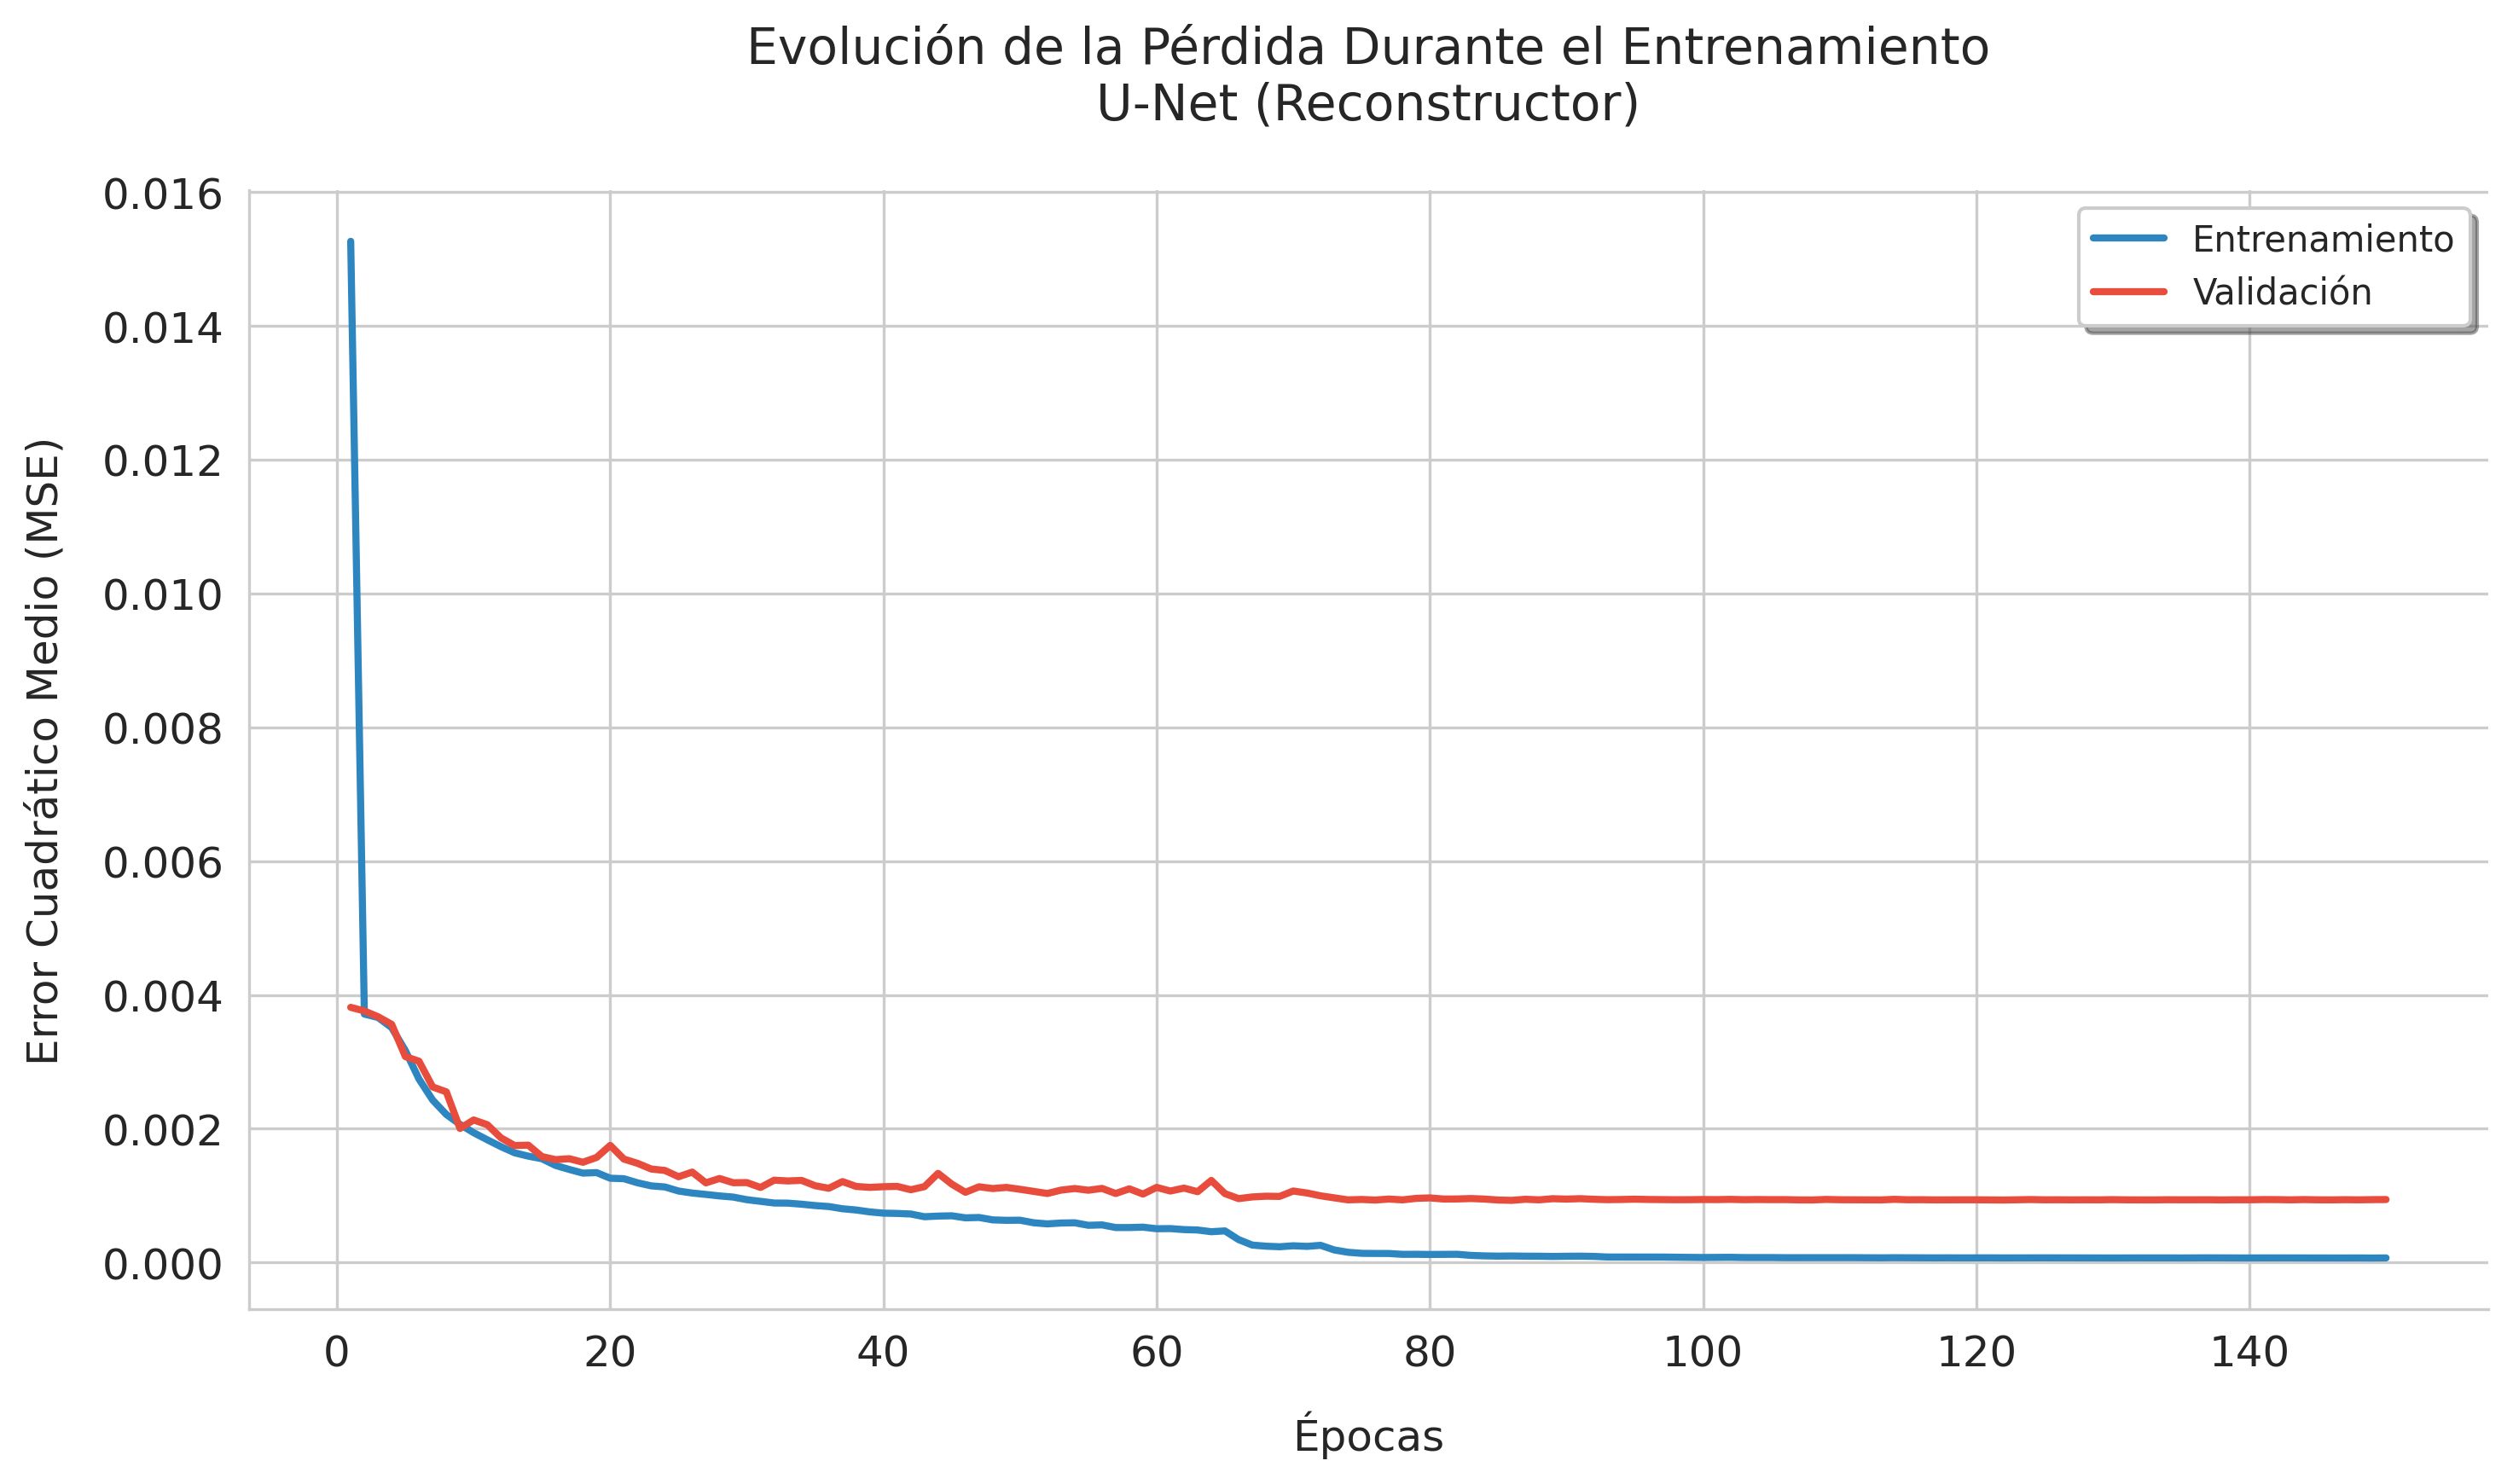
\includegraphics[width=0.8\textwidth]{Images/perdidas_entrenamiento_recon.png}
    \caption{Evolución de la función de pérdida durante el preentrenamiento de la red reconstructora.}
    \label{fig:reconstructor_pretraining}
\end{figure}

\subsubsection{Red Supervisora}

El segundo paso fue entrenar la red supervisora con los hiperparámetros especificados en la sección \ref{subsubsec:pretraining}. La Figura \ref{fig:supervisor_pretraining} muestra la evolución de la función de pérdida durante el entrenamiento. Se observa que la función de pérdida inicia en valores cercanos a 1.0 MSE y disminuye rápidamente durante las primeras épocas. Sin embargo, la curva de validación presenta fluctuaciones considerables durante el proceso de entrenamiento, convergiendo finalmente a un nivel de error más elevado (aproximadamente 0.1 MSE). La brecha más pronunciada entre las pérdidas de entrenamiento y validación, junto con las oscilaciones persistentes, sugieren que la tarea de supervisión presenta mayores desafíos en términos de generalización que la tarea de reconstrucción.

\begin{figure}[H]
    \centering
    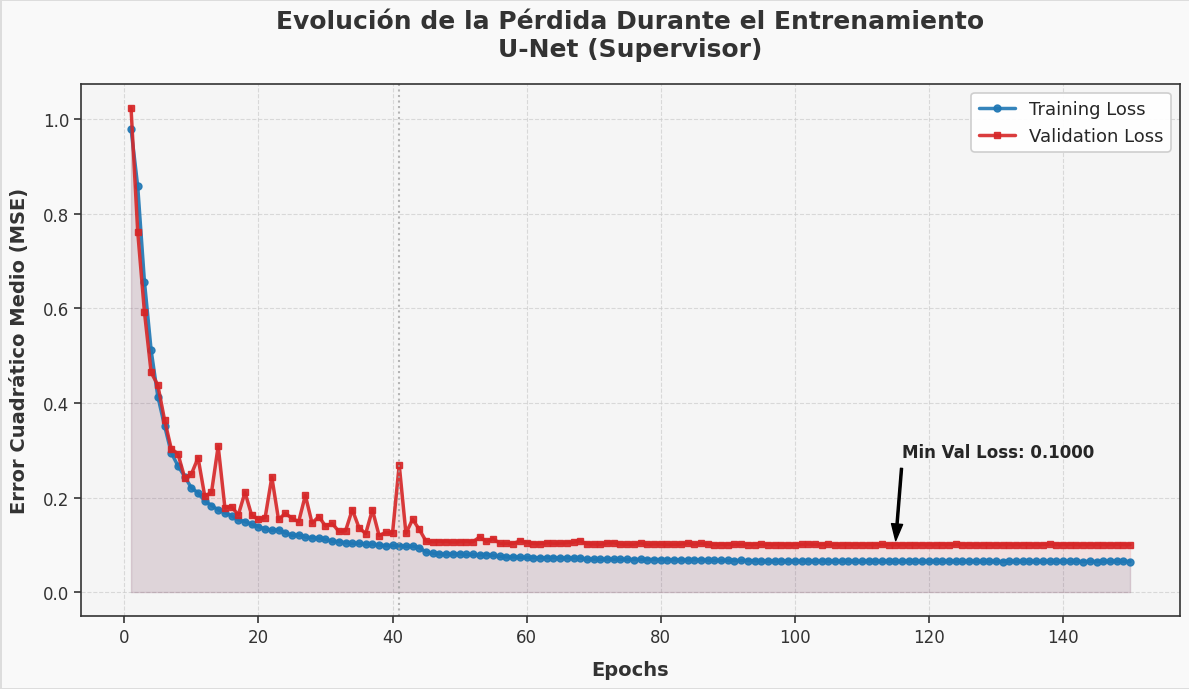
\includegraphics[width=0.8\textwidth]{Images/perdidas_entrenamiento_super.png}
    \caption{Evolución de la función de pérdida durante el preentrenamiento de la red supervisora.}
    \label{fig:supervisor_pretraining}
\end{figure}

\subsection{Fine-tuning}

Para evaluar la metodología propuesta, se realizó el fine-tuning de la red constructora con los hiperparámetros especificados en la sección \ref{subsubsec:pretraining}. Se comparan los resultados obtenidos con la metodología propuesta con los obtenidos al entrenar solo la U-Net. Además, se evalúa la importancia de cada componente de la función de pérdida propuesta al eliminarlo del finetuning.

\subsubsection{Metodología propuesta vs. U-Net}

Primero observamos los resultados obtenidos en el proceso del fine-tuning de la red reconstructora. La Figura \ref{fig:reconstructor_finetuning} muestra la evolución de la función de pérdida durante el entrenamiento. 

\begin{figure}[H]
    \centering
    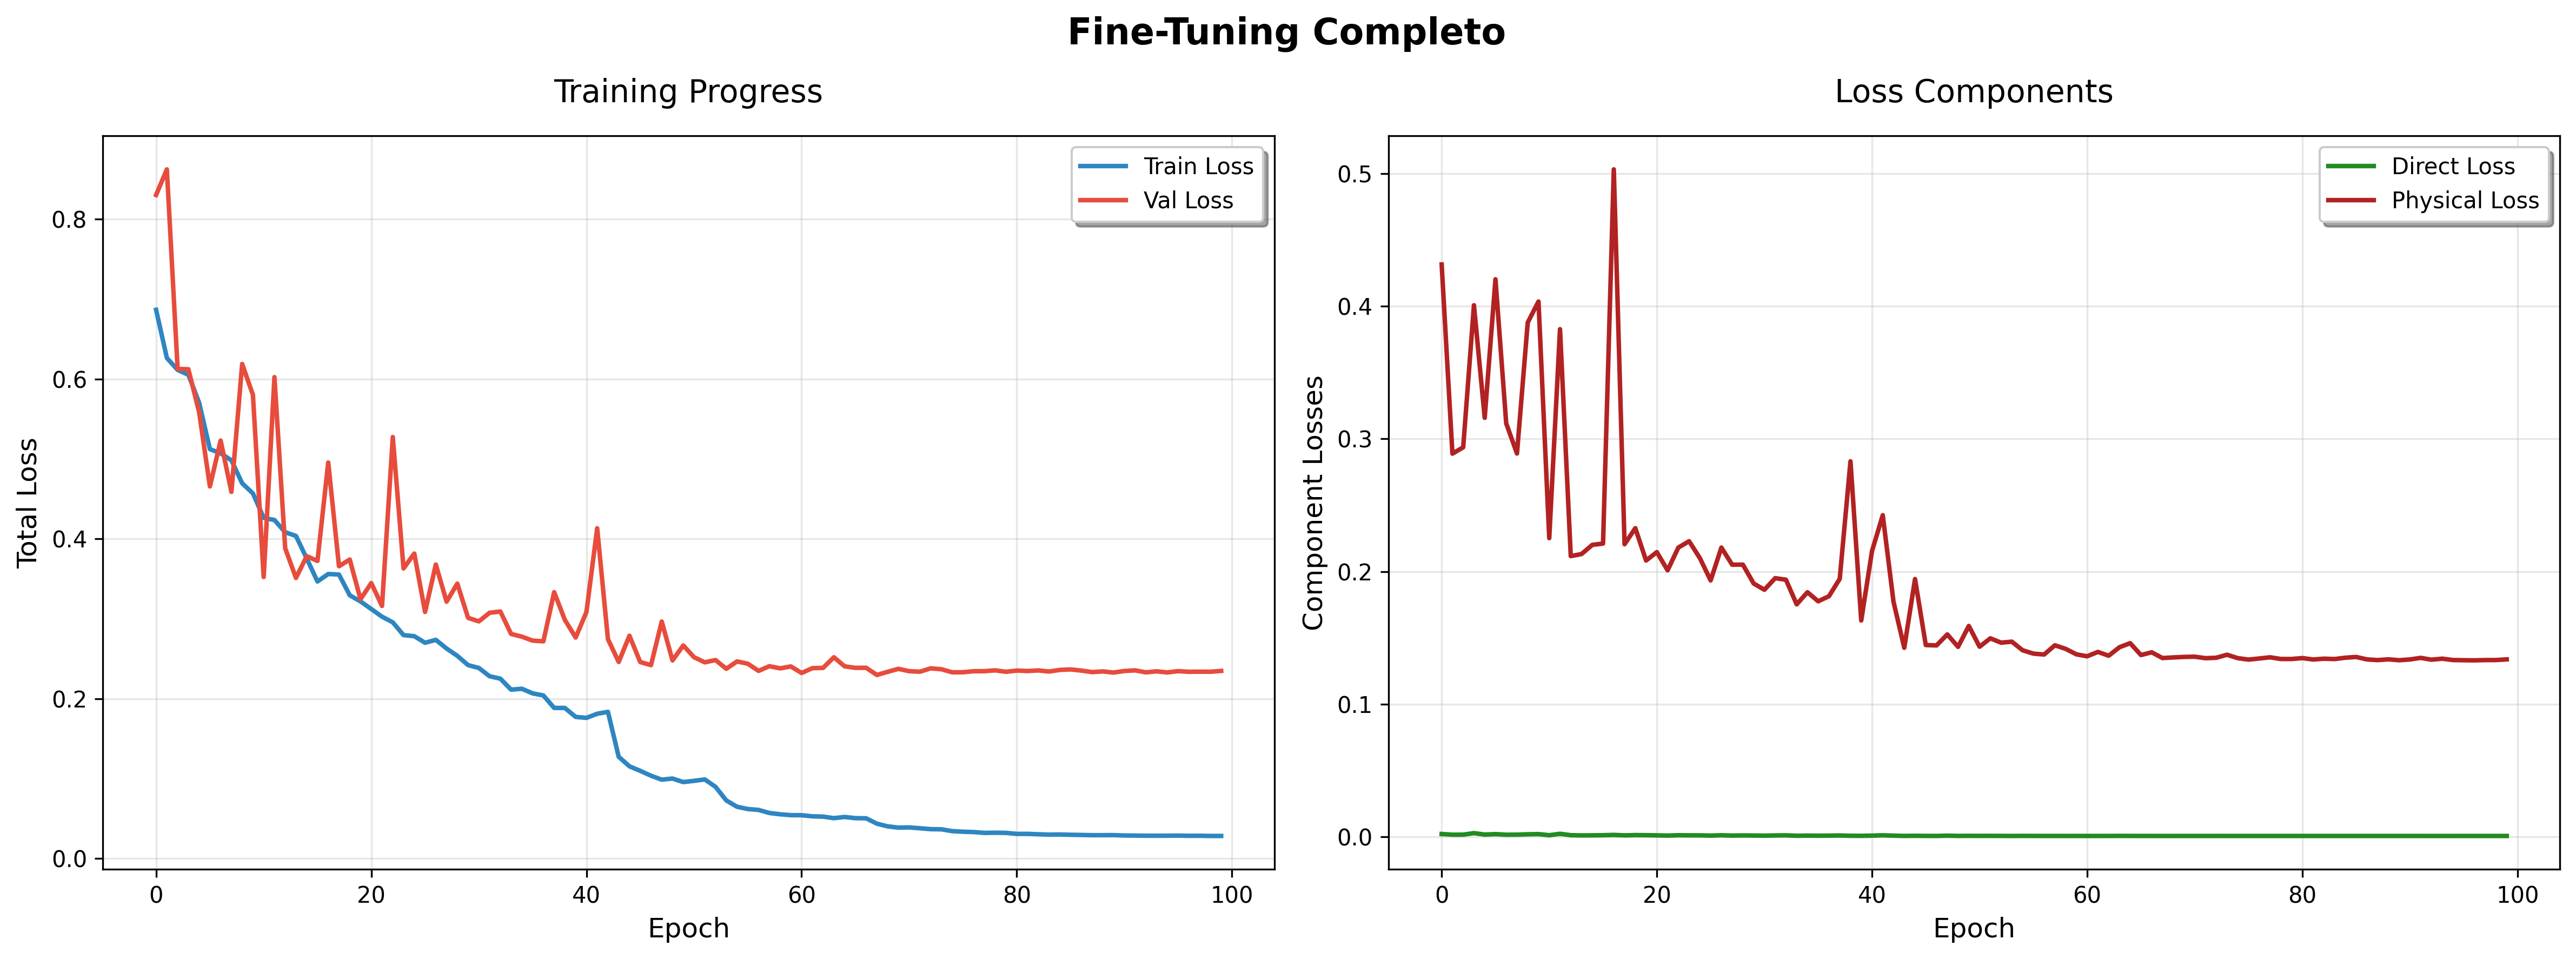
\includegraphics[width=0.8\textwidth]{Images/perdidas_entrenamiento_finetuning.png}
    \caption{Evolución de la función de pérdida durante el fine-tuning de la red reconstructora.}
    \label{fig:reconstructor_finetuning}
\end{figure}

La gráfica de evolución de pérdidas durante el fine-tuning muestra dos componentes principales: la pérdida directa (reconstrucción) y la pérdida física. La pérdida directa, heredada del preentrenamiento del reconstructor U-Net, se mantiene consistentemente baja (cercana a 0.005) durante todo el proceso, indicando que la red mantiene su capacidad de reconstrucción de imágenes.
La pérdida física, por otro lado, inicia con valores altos (~0.4-0.5) y muestra alta volatilidad en las primeras 20 épocas. Posteriormente, se estabiliza gradualmente hasta converger alrededor de 0.13. Esta evolución sugiere que la red está aprendiendo progresivamente a satisfacer las restricciones físicas sin comprometer significativamente su capacidad de reconstrucción original.
La curva de pérdida total muestra una brecha entre entrenamiento y validación similar a lo observado en el supervisor, con el entrenamiento convergiendo a ~0.05 y la validación a ~0.2, lo cual es esperado dado el componente físico añadido.


\subsubsection{Ablación de componentes de la función de pérdida} \label{subsec:ablation}

Como bien esta descrito en la sección \ref{subsubsec:pretraining}, la función de pérdida propuesta consta de cuatro componentes: pérdida directa, pérdida física, pérdida estructural y pérdida de similitud, donde la pérdida estructural tiene un gran peso sobre los demás componentes. Para evaluar la importancia de cada componente en la función de pérdida, se realizaron experimentos de ablación eliminando cada componente de la función de pérdida mientras se mantenían los demás términos constantes. Los resultados obtenidos durante el fine-tuning de la red constructora se muestran en la Figura \ref{fig:ablation_no_struct} y \ref{fig:ablation_no_phys}.

\begin{figure}[H]
    \centering
    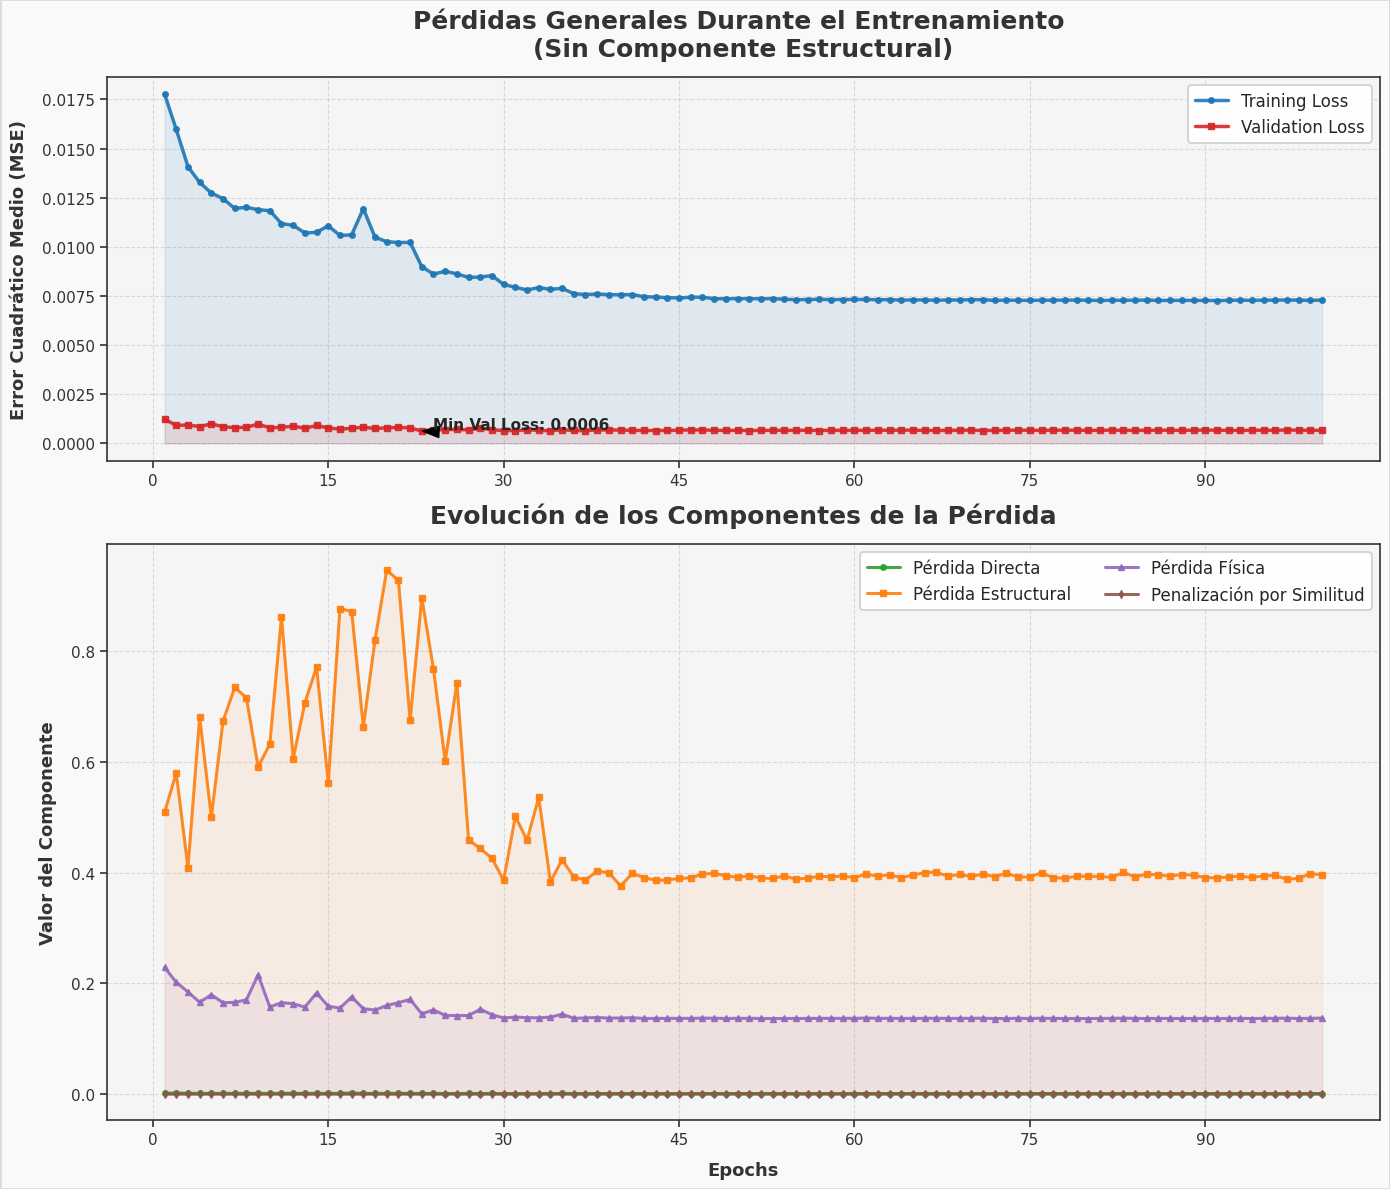
\includegraphics[width=0.8\textwidth]{Images/perdidas_entrenamiento_finetuning_no_struct.png}
    \caption{Evolución de la función de pérdida durante el fine-tuning de la red constructora eliminando la pérdida estructural.}
    \label{fig:ablation_no_struct}
\end{figure}

\begin{figure}[H]
    \centering
    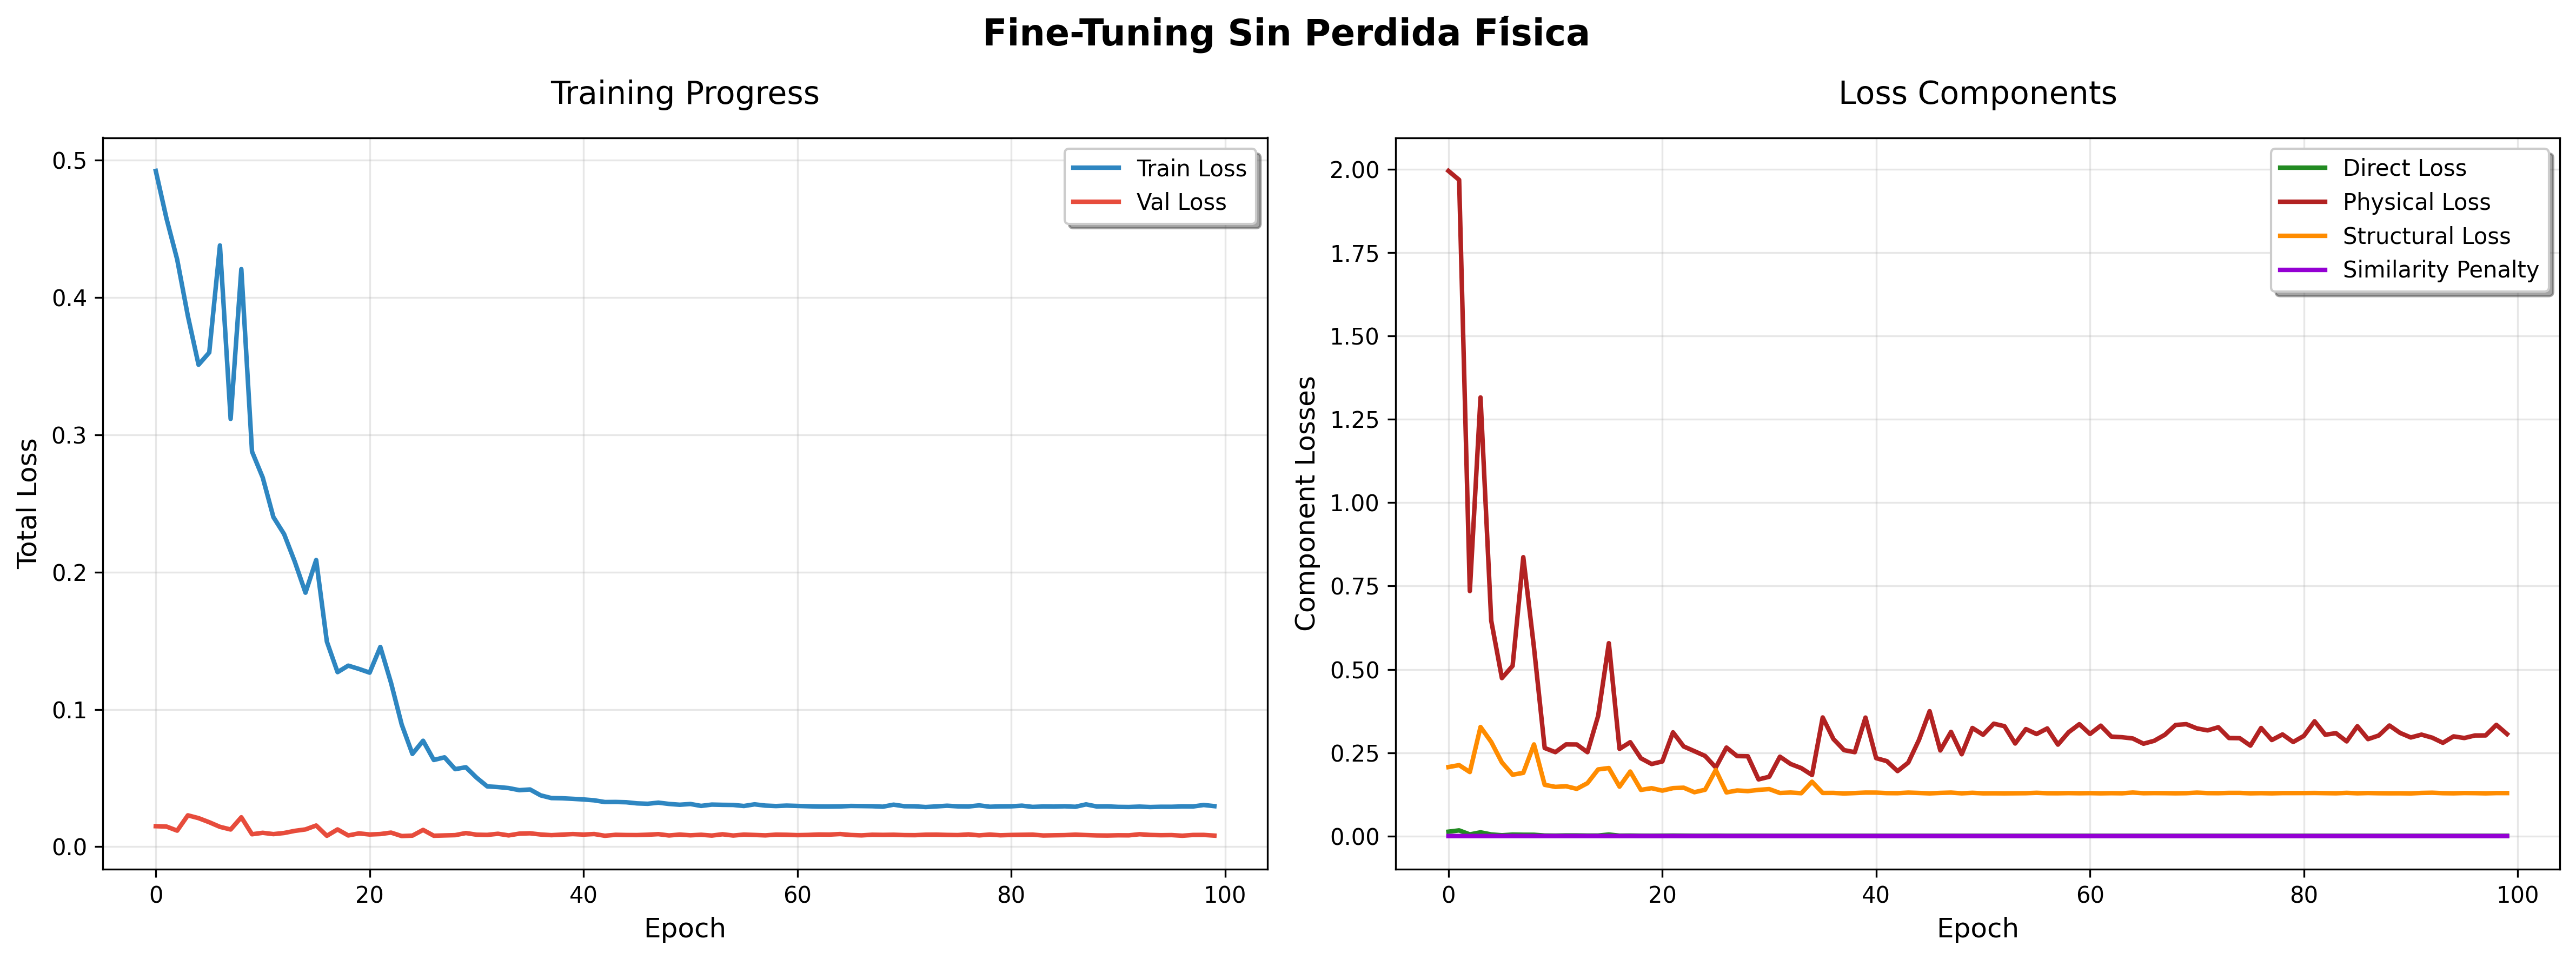
\includegraphics[width=0.8\textwidth]{Images/perdidas_entrenamiento_finetuning_no_phy.png}
    \caption{Evolución de la función de pérdida durante el fine-tuning de la red constructora eliminando la pérdida física.}
    \label{fig:ablation_no_phys}
\end{figure}

El análisis de las gráficas de fine-tuning revela comportamientos distintivos al eliminar diferentes componentes de pérdida. En el caso sin pérdida estructural, observamos una pérdida total inicial de aproximadamente 0.5 que converge gradualmente a 0.03. La pérdida física muestra una dinámica particularmente interesante, comenzando en valores cercanos a 2.0 con oscilaciones pronunciadas en las primeras 20 épocas, antes de estabilizarse alrededor de 0.3. Las pérdidas directa y de similitud se mantienen consistentemente cercanas a cero, aunque se observa una brecha notable entre las curvas de entrenamiento y validación.

Por otro lado, cuando se elimina la pérdida física, el comportamiento del modelo cambia significativamente. La pérdida total se mantiene en un rango mucho menor, iniciando en aproximadamente 0.0175. La pérdida estructural se convierte en el componente dominante, mostrando un patrón distintivo donde aumenta inicialmente hasta alcanzar un pico de 0.8 alrededor de la época 20, para luego estabilizarse en aproximadamente 0.4. Es notable que la pérdida directa y la pérdida de similitud se mantienen excepcionalmente bajas (~0.001), sugiriendo que el modelo preserva su capacidad de reconstrucción básica. La convergencia en este caso es más suave y estable en comparación con el escenario sin pérdida estructural, indicando una optimización más consistente del modelo.

\subsection{Metricas de evaluación}

Para evaluar la calidad de las imágenes generadas por la red reconstructora, se utilizaron las métricas de evaluación descritas en la sección \ref{sec:metrics}. Las métricas de evaluación se calcularon para las imágenes generadas por la red reconstructora en el conjunto de prueba. Los resultados obtenidos se muestran en la Tabla \ref{tab:metricas}.

\begin{table}[H]
    \centering
    \begin{tabularx}{\textwidth}{lXXXXXX}
    \hline
    \textbf{Modelo} & \textbf{MSE} & \textbf{MAE} & \textbf{NRMSE} & \textbf{PSNR} (dB) & \textbf{SSIM} \\
    \hline
    Baseline & $9\times10^{-3} \pm 0.0005$ & $3\times10^{-2} \pm 0.002$ & $4\times10^{-1} \pm 0.01$ & $29.0 \pm 2.0$ & $0.96 \pm 0.01$ \\
    FT & $7\times10^{-3} \pm 0.0006$ & $2\times10^{-2} \pm 0.002$ & $3\times10^{-1} \pm 0.03$ & $30.0 \pm 3.0$ & $0.97 \pm 0.01$ \\
    FT No-Physical & $1\times10^{-2} \pm 0.0008$ & $4\times10^{-2} \pm 0.003$ & $4\times10^{-1} \pm 0.03$ & $28.0 \pm 3.0$ & $0.95 \pm 0.01$ \\
    FT No-Structural & $1\times10^{-2} \pm 0.001$ & $1\times10^{-1} \pm 0.001$ & $4\times10^{-1} \pm 0.04$ & $27.0 \pm 2.0$ & $0.62 \pm 0.1$ \\
    \hline
    \end{tabularx}
    \caption{Métricas de evaluación de las imágenes generadas por la red reconstructora en el conjunto de prueba. Los valores incluyen las desviaciones estándar.}
    \label{tab:metricas}
\end{table}

En las siguientes secciones se profundiza en cada una de estas metricas y se comparan los resultados obtenidos con la metodología propuesta con los obtenidos al entrenar solo la U-Net. Además, se evalúa la importancia de cada componente de la función de pérdida propuesta al eliminarlo del finetuning.

\subsubsection{Error Absoluto Medio (MAE)}

El Error Absoluto Medio (MAE) proporciona una medida directa de la magnitud promedio de los errores de reconstrucción. La Figura \ref{fig:mae_analysis} presenta un análisis comparativo entre el modelo pre-entrenado y las tres variantes de fine-tuning implementadas.

\begin{figure}[H]
    \centering
    \begin{subfigure}[b]{0.48\textwidth}
        \centering
        % FT No-Physical vs Baseline
        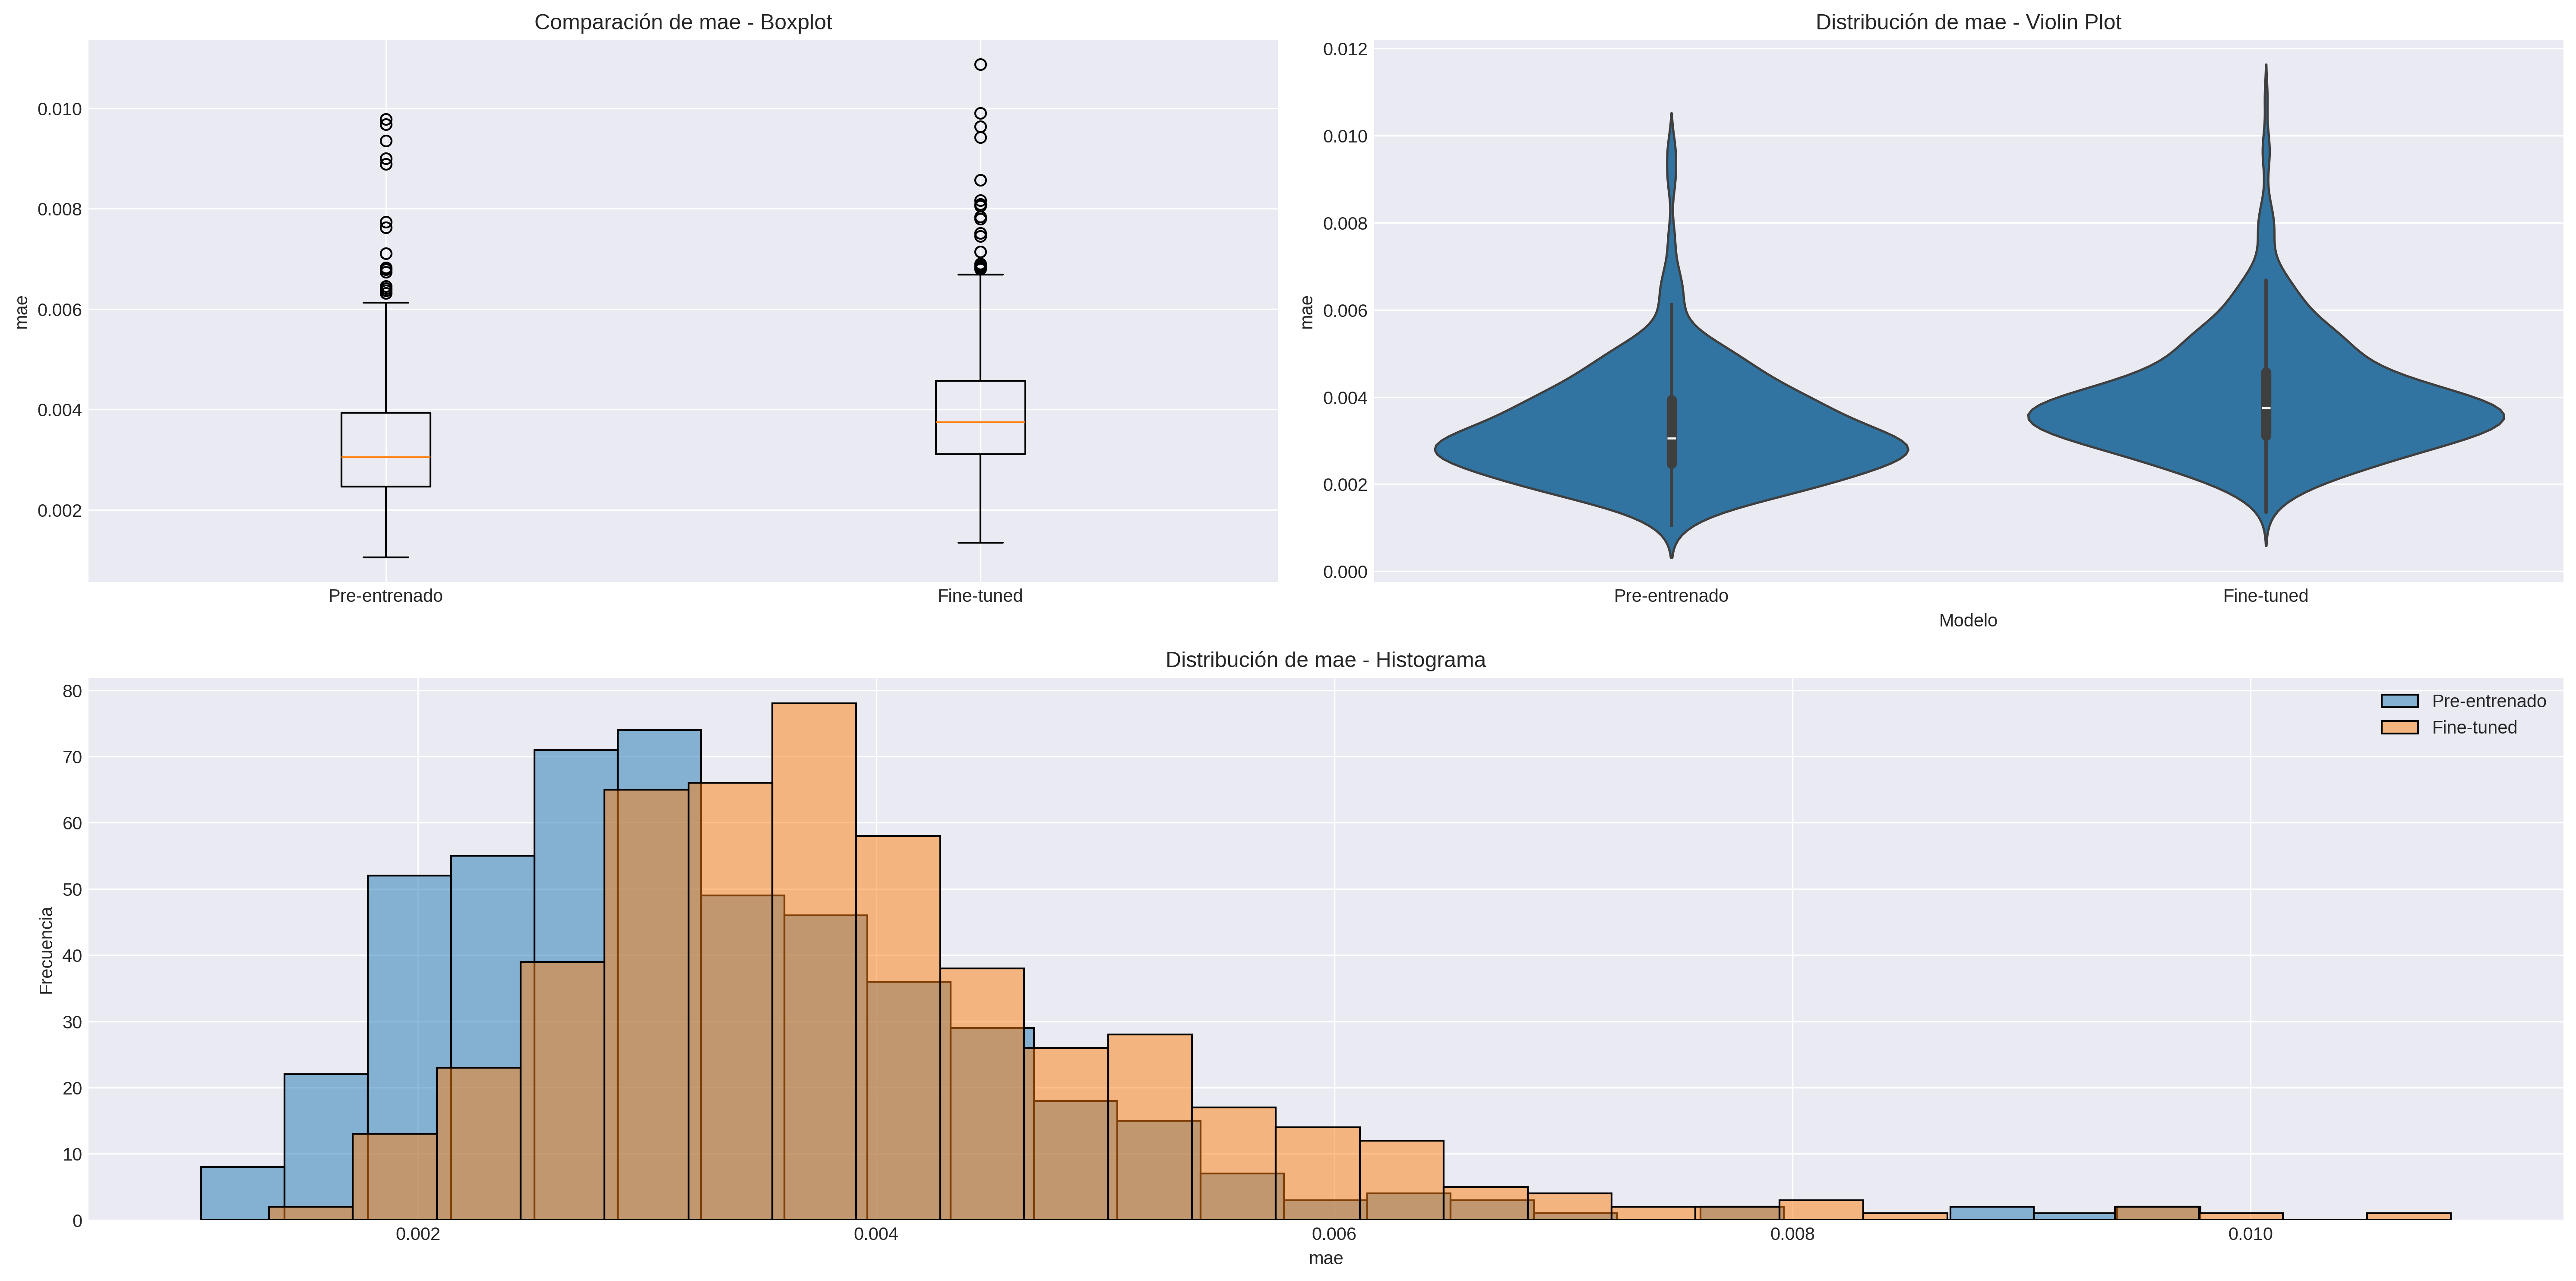
\includegraphics[width=\textwidth]{Images/comparison_plots_mae_no_phy.png}
        \caption{Comparación entre fine-tuning sin componente física y modelo pre-entrenado}
        \label{fig:mae_hist}
    \end{subfigure}
    \hfill
    \begin{subfigure}[b]{0.48\textwidth}
        \centering
        % FT No-Structural vs Baseline
        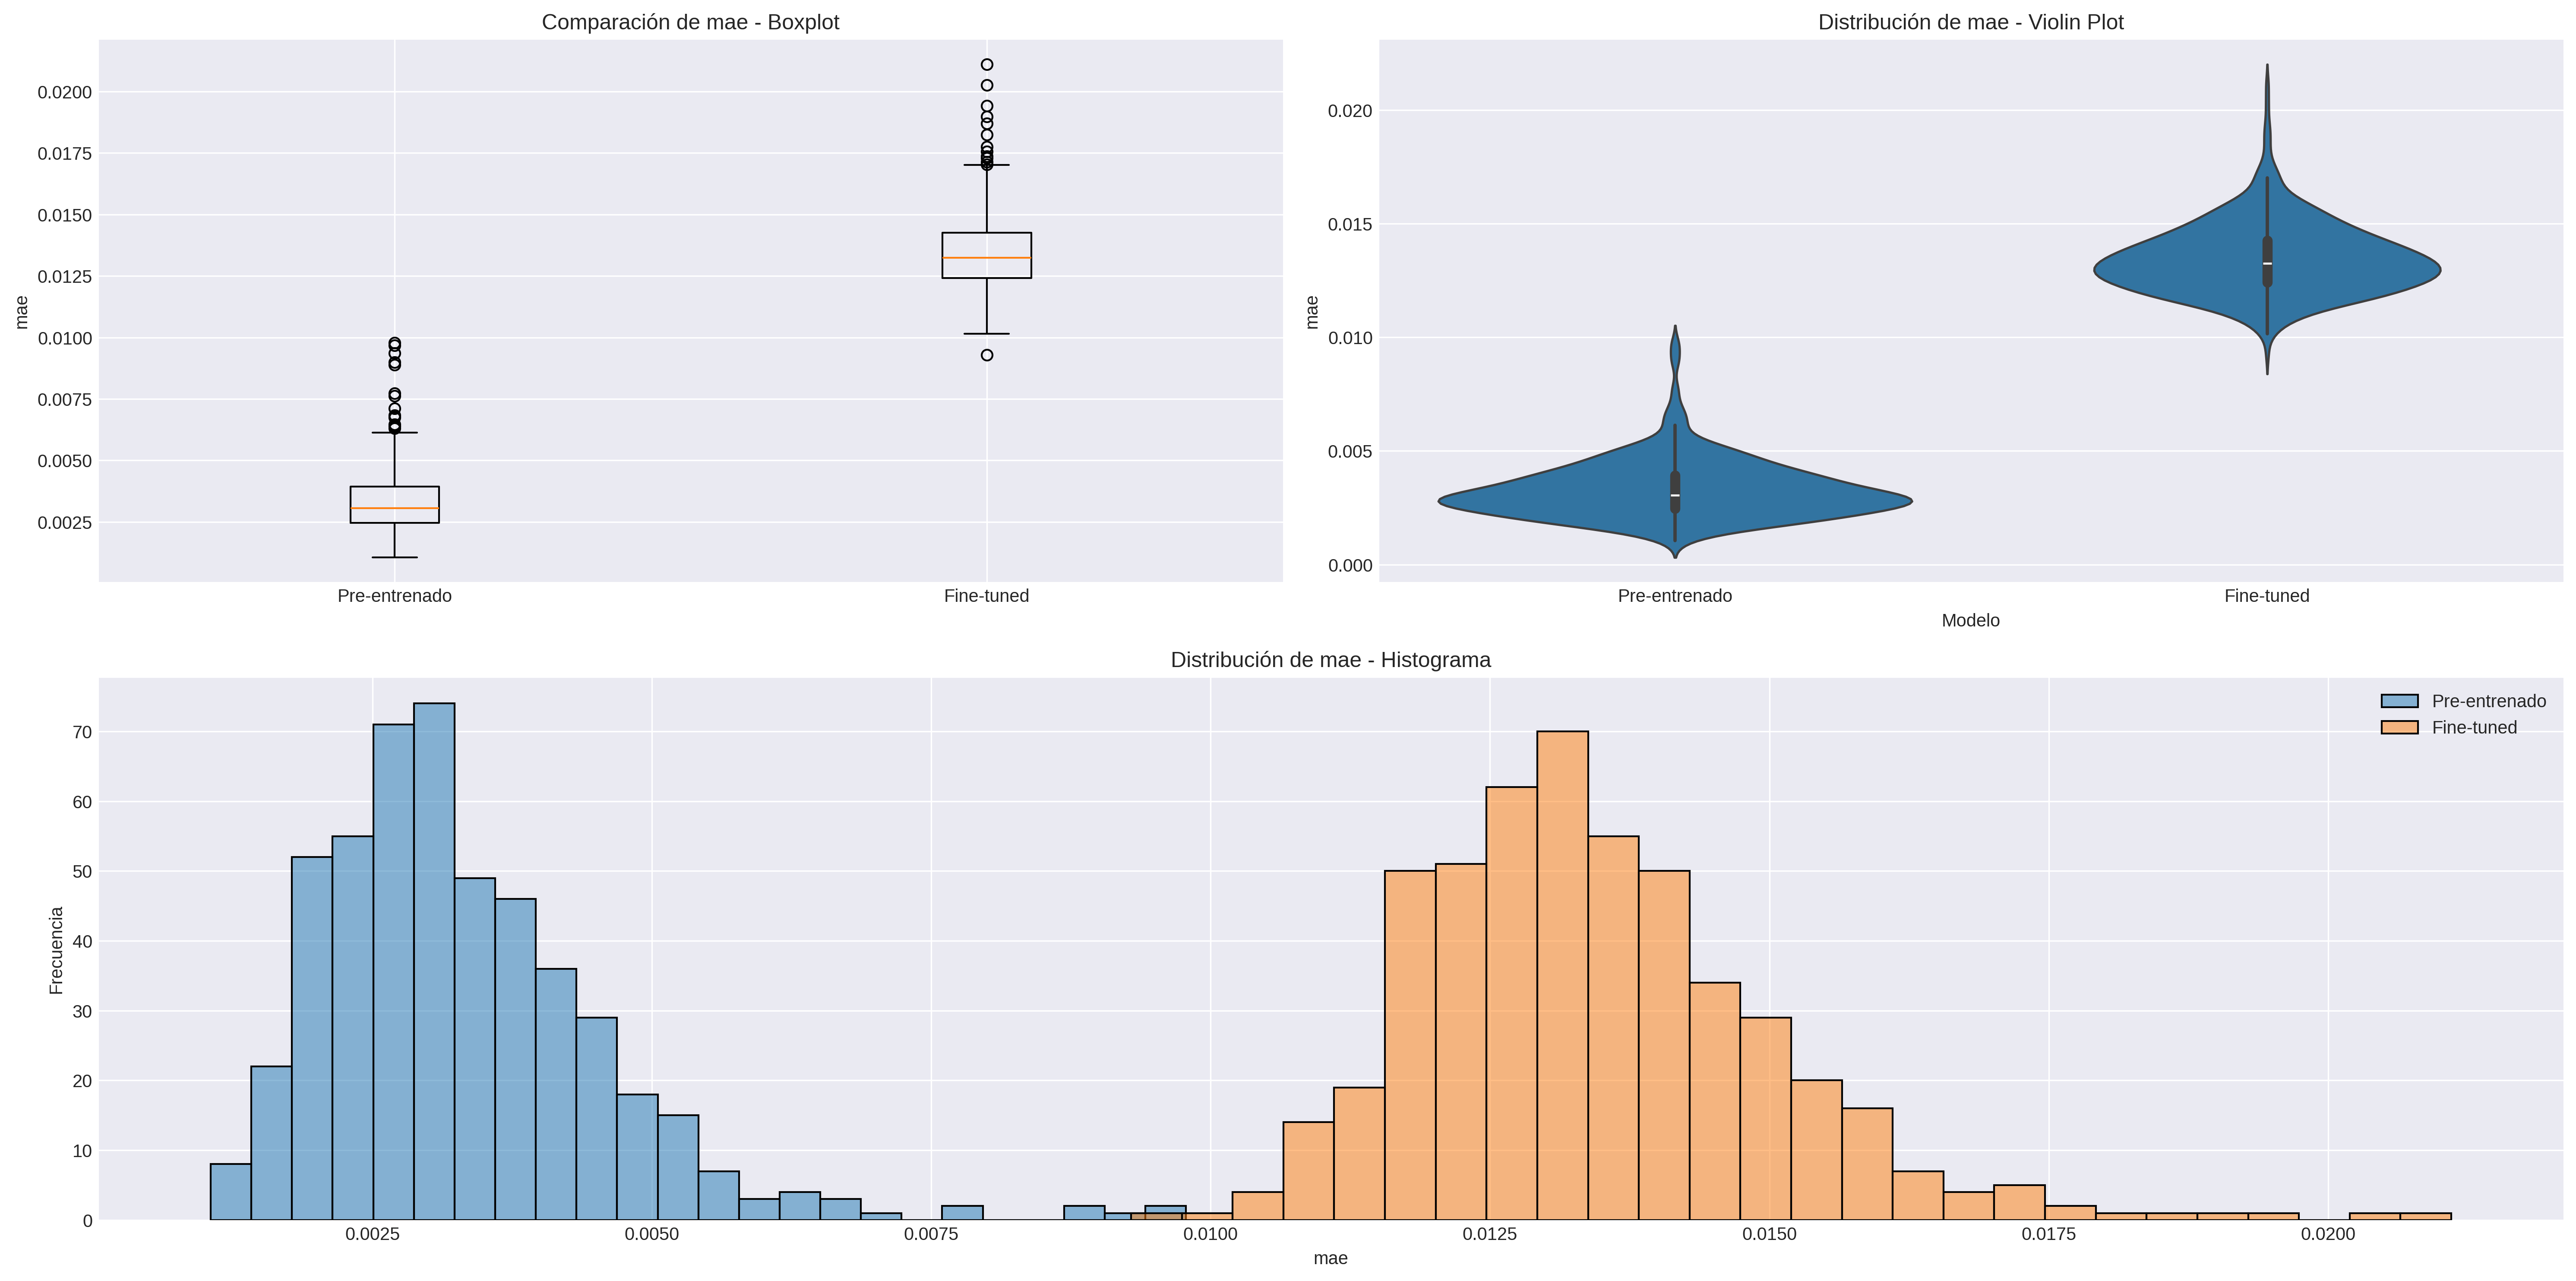
\includegraphics[width=\textwidth]{Images/comparison_plots_mae_no_struct.png}
        \caption{Comparación entre fine-tuning sin componente estructural y modelo pre-entrenado}
        \label{fig:mae_violin}
    \end{subfigure}
    
    \vspace{0.5cm}
    
    \begin{subfigure}[b]{0.7\textwidth}
        \centering
        % FT vs Baseline
        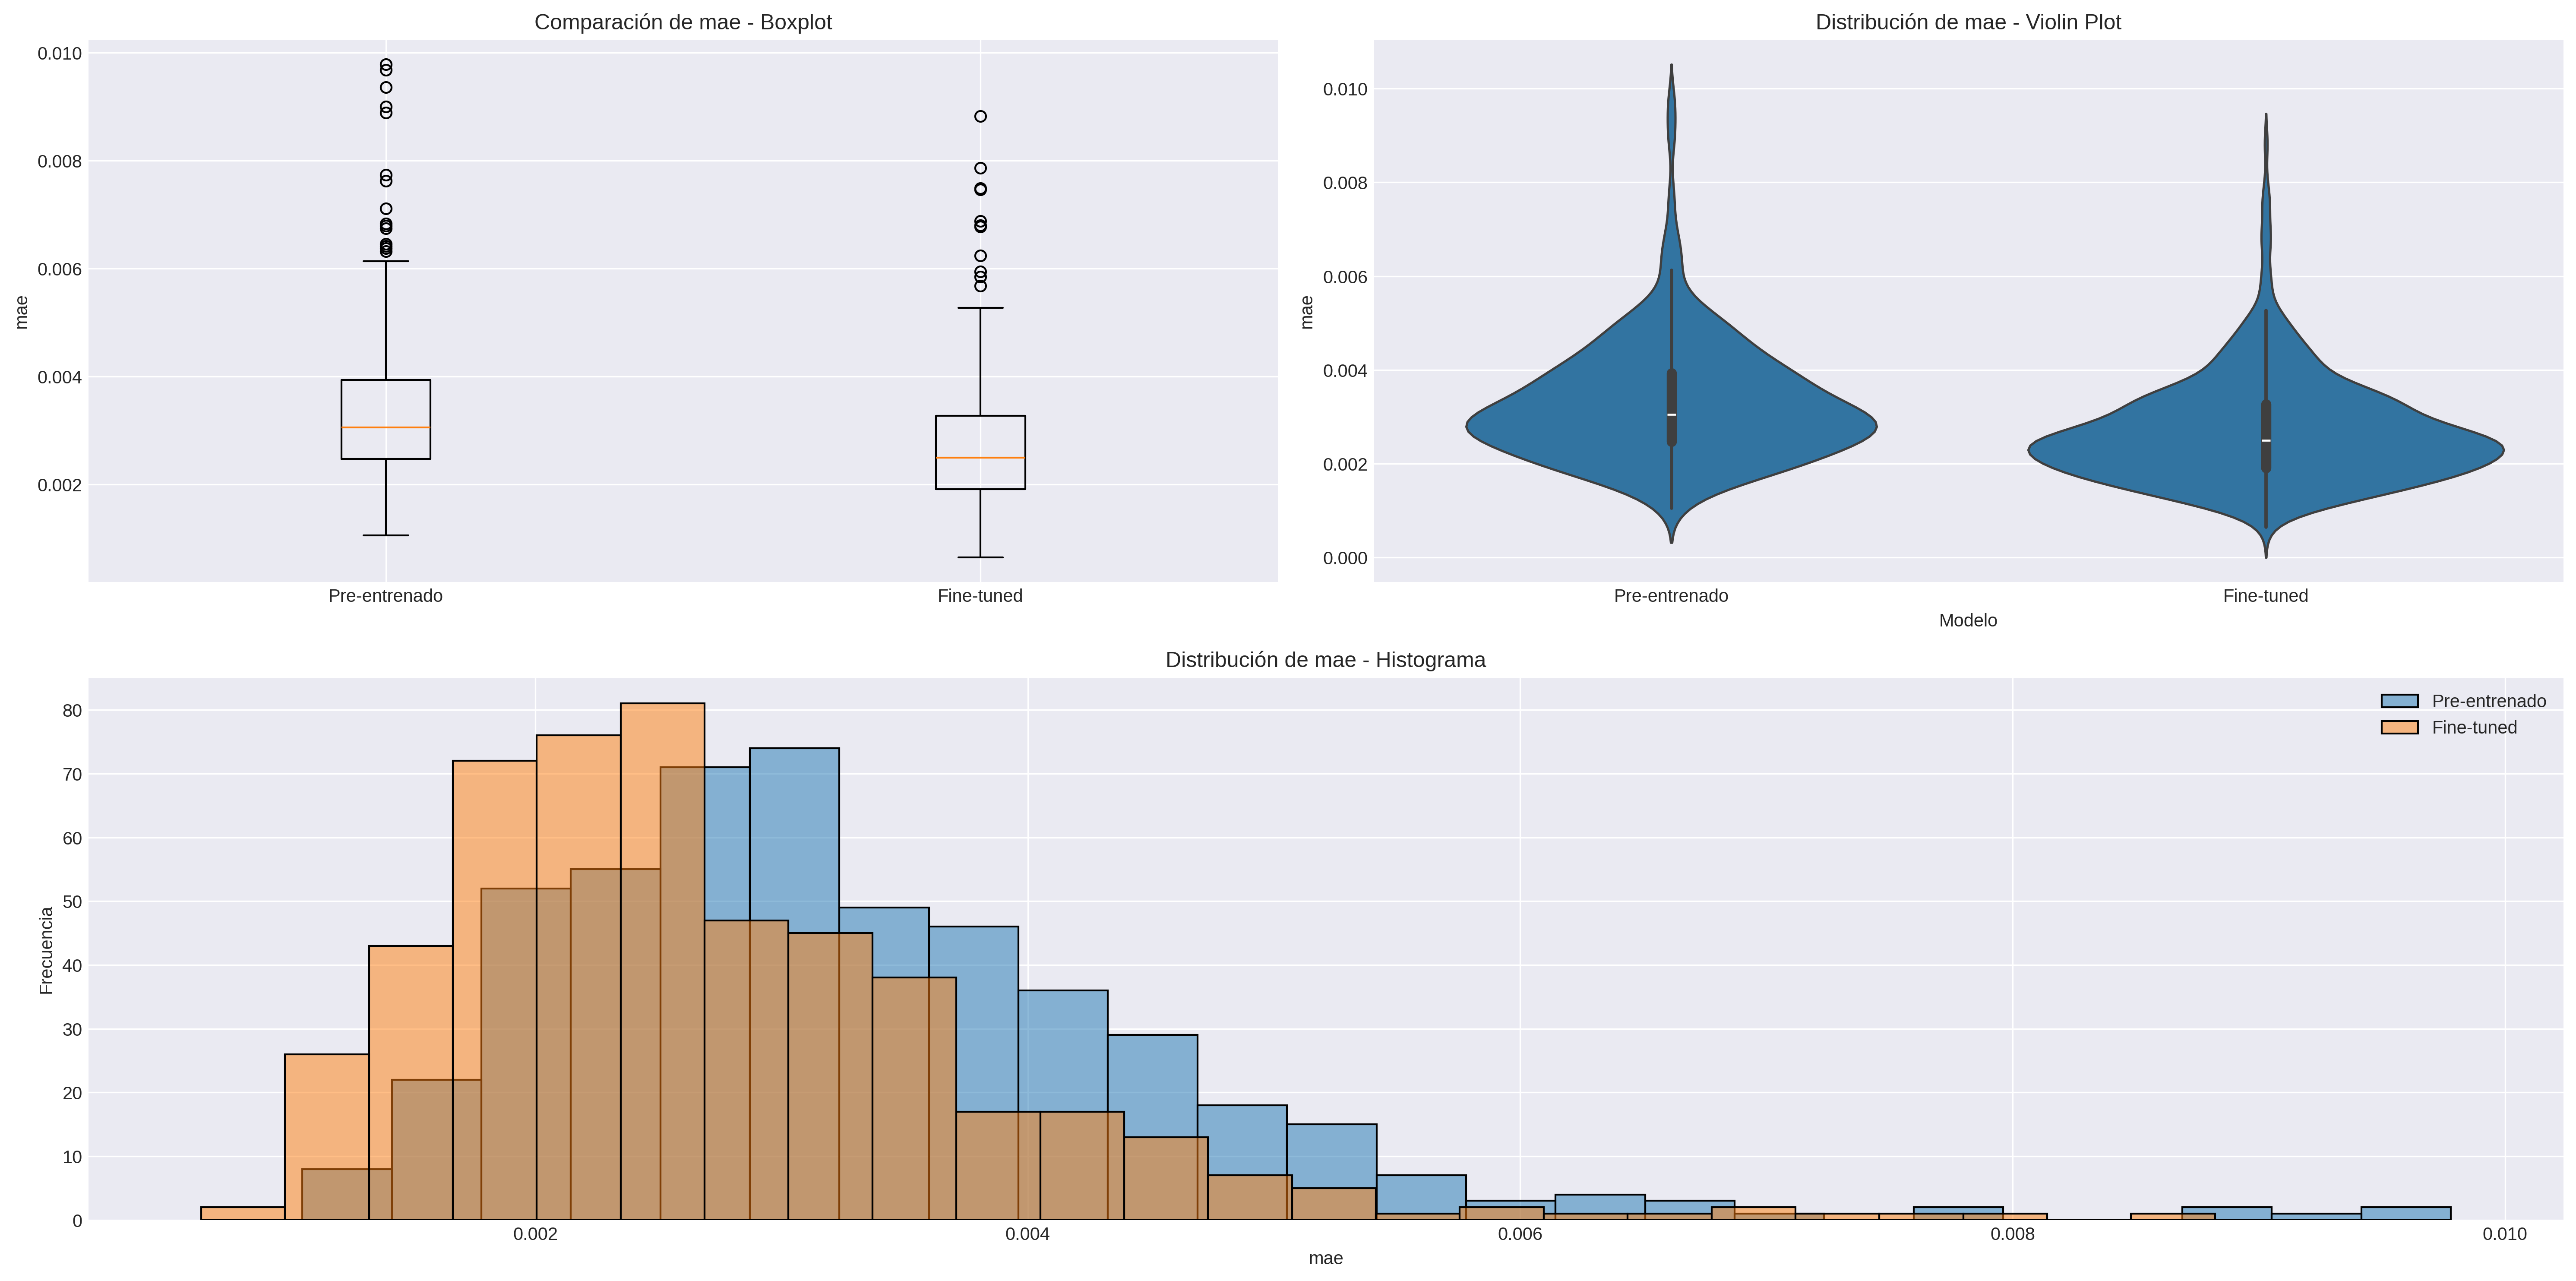
\includegraphics[width=\textwidth]{Images/comparison_plots_mae_sup.png}
        \caption{Comparación entre fine-tuning (FT) completo y modelo pre-entrenado}
        \label{fig:mae_box}
    \end{subfigure}
    
    \caption{Análisis comparativo del Error Absoluto Medio (MAE) entre el modelo pre-entrenado y las variantes de fine-tuning implementadas. a) Comparación entre fine-tuning sin componente física y modelo pre-entrenado. b) Comparación entre fine-tuning sin componente estructural y modelo pre-entrenado. c) Comparación entre fine-tuning completo y modelo pre-entrenado.}
    \label{fig:mae_analysis}
\end{figure}


\paragraph{Fine-tuning Completo (FT)}
El modelo con fine-tuning completo demuestra una mejora significativa en el rendimiento respecto al modelo pre-entrenado. El MAE medio se redujo de $3.301 \times 10^{-3}$ (pre-entrenado) a $2.690 \times 10^{-3}$ (fine-tuned), representando una mejora del 18.50\%. La dispersión de los errores también se redujo, como lo evidencia la disminución en la desviación estándar de $1.276 \times 10^{-3}$ a $1.114 \times 10^{-3}$. El rango de errores se contrajo, con el valor mínimo mejorando de $1.054 \times 10^{-3}$ a $0.643 \times 10^{-3}$ y el máximo reduciéndose de $9.780 \times 10^{-3}$ a $8.822 \times 10^{-3}$.

La significancia estadística de esta mejora se confirma mediante múltiples pruebas. Aunque las pruebas de Shapiro-Wilk ($W = 0.9027$ y $W = 0.9006$, ambas con $p < 0.001$) indican que las distribuciones no son normales, tanto la prueba t pareada ($t = 19.6755$, $p < 0.001$) como la prueba no paramétrica de Wilcoxon ($W = 10619.0000, p < 0.001$) confirman que la diferencia es estadísticamente significativa. El tamaño del efecto ($d$ de $Cohen = 0.5099$) indica una mejora prácticamente significativa de magnitud media a grande.

\paragraph{Fine-tuning sin Componente Física (FT No-Physical)}
La eliminación de la componente física en el fine-tuning resulta en un deterioro significativo del rendimiento. El MAE medio aumentó a $3.975 \times 10^{-3}$, representando un incremento del 20.42\% respecto al modelo pre-entrenado ($3.301 \times 10^{-3}$). La variabilidad de los errores también aumentó, con una desviación estándar de $1.321 \times 10^{-3}$. El rango de errores se expandió, con un valor mínimo de $1.349 \times 10^{-3}$ y un máximo de $10.873 \times 10^{-3}$.

Las pruebas estadísticas confirman el impacto negativo de eliminar la componente física. La prueba t pareada ($t = -27.5056$, $p < 0.001$) y la prueba de Wilcoxon ($W = 4313.0000$, $p < 0.001$) indican que el deterioro es estadísticamente significativo. El tamaño del efecto negativo ($d$ de $Cohen = -0.5192$) sugiere que la ausencia de la componente física tiene un impacto sustancial en el rendimiento del modelo.

\paragraph{Fine-tuning sin Componente Estructural (FT No-Structural)}
La ausencia de la componente estructural produce el deterioro más severo en el rendimiento del modelo. El MAE medio se incrementó dramáticamente a $13.438 \times 10^{-3}$, representando un empeoramiento del 307.08\% respecto al modelo pre-entrenado. La dispersión de los errores aumentó significativamente, con una desviación estándar de $1.559 \times 10^{-3}$. El rango de errores se expandió considerablemente, con un valor mínimo de $9.289 \times 10^{-3}$ y un máximo de $21.101 \times 10^{-3}$.

El análisis estadístico revela la magnitud del impacto negativo. Las pruebas de significancia muestran diferencias extremadamente significativas, con un estadístico $t$ de $-269.9921$ ($p < 0.001$) y un estadístico de Wilcoxon $W = 0 (p < 0.001)$. El tamaño del efecto es notablemente grande y negativo ($d$ de $Cohen = -7.1154$), indicando que la componente estructural es crucial para el rendimiento del modelo. Esta degradación sustancial en el rendimiento subraya la importancia fundamental de la componente estructural en la función de pérdida.

\subsubsection{Error Cuadrático Medio (MSE)}

El Error Cuadrático Medio (MSE) proporciona una medida cuantitativa de la magnitud promedio de los errores de reconstrucción. La Figura \ref{fig:mse_analysis} presenta un análisis comparativo entre el modelo pre-entrenado y las tres variantes de fine-tuning implementadas.

\begin{figure}
    \begin{figure}[H]
        \centering
        \begin{subfigure}[b]{0.48\textwidth}
            \centering
            % FT No-Physical vs Baseline
            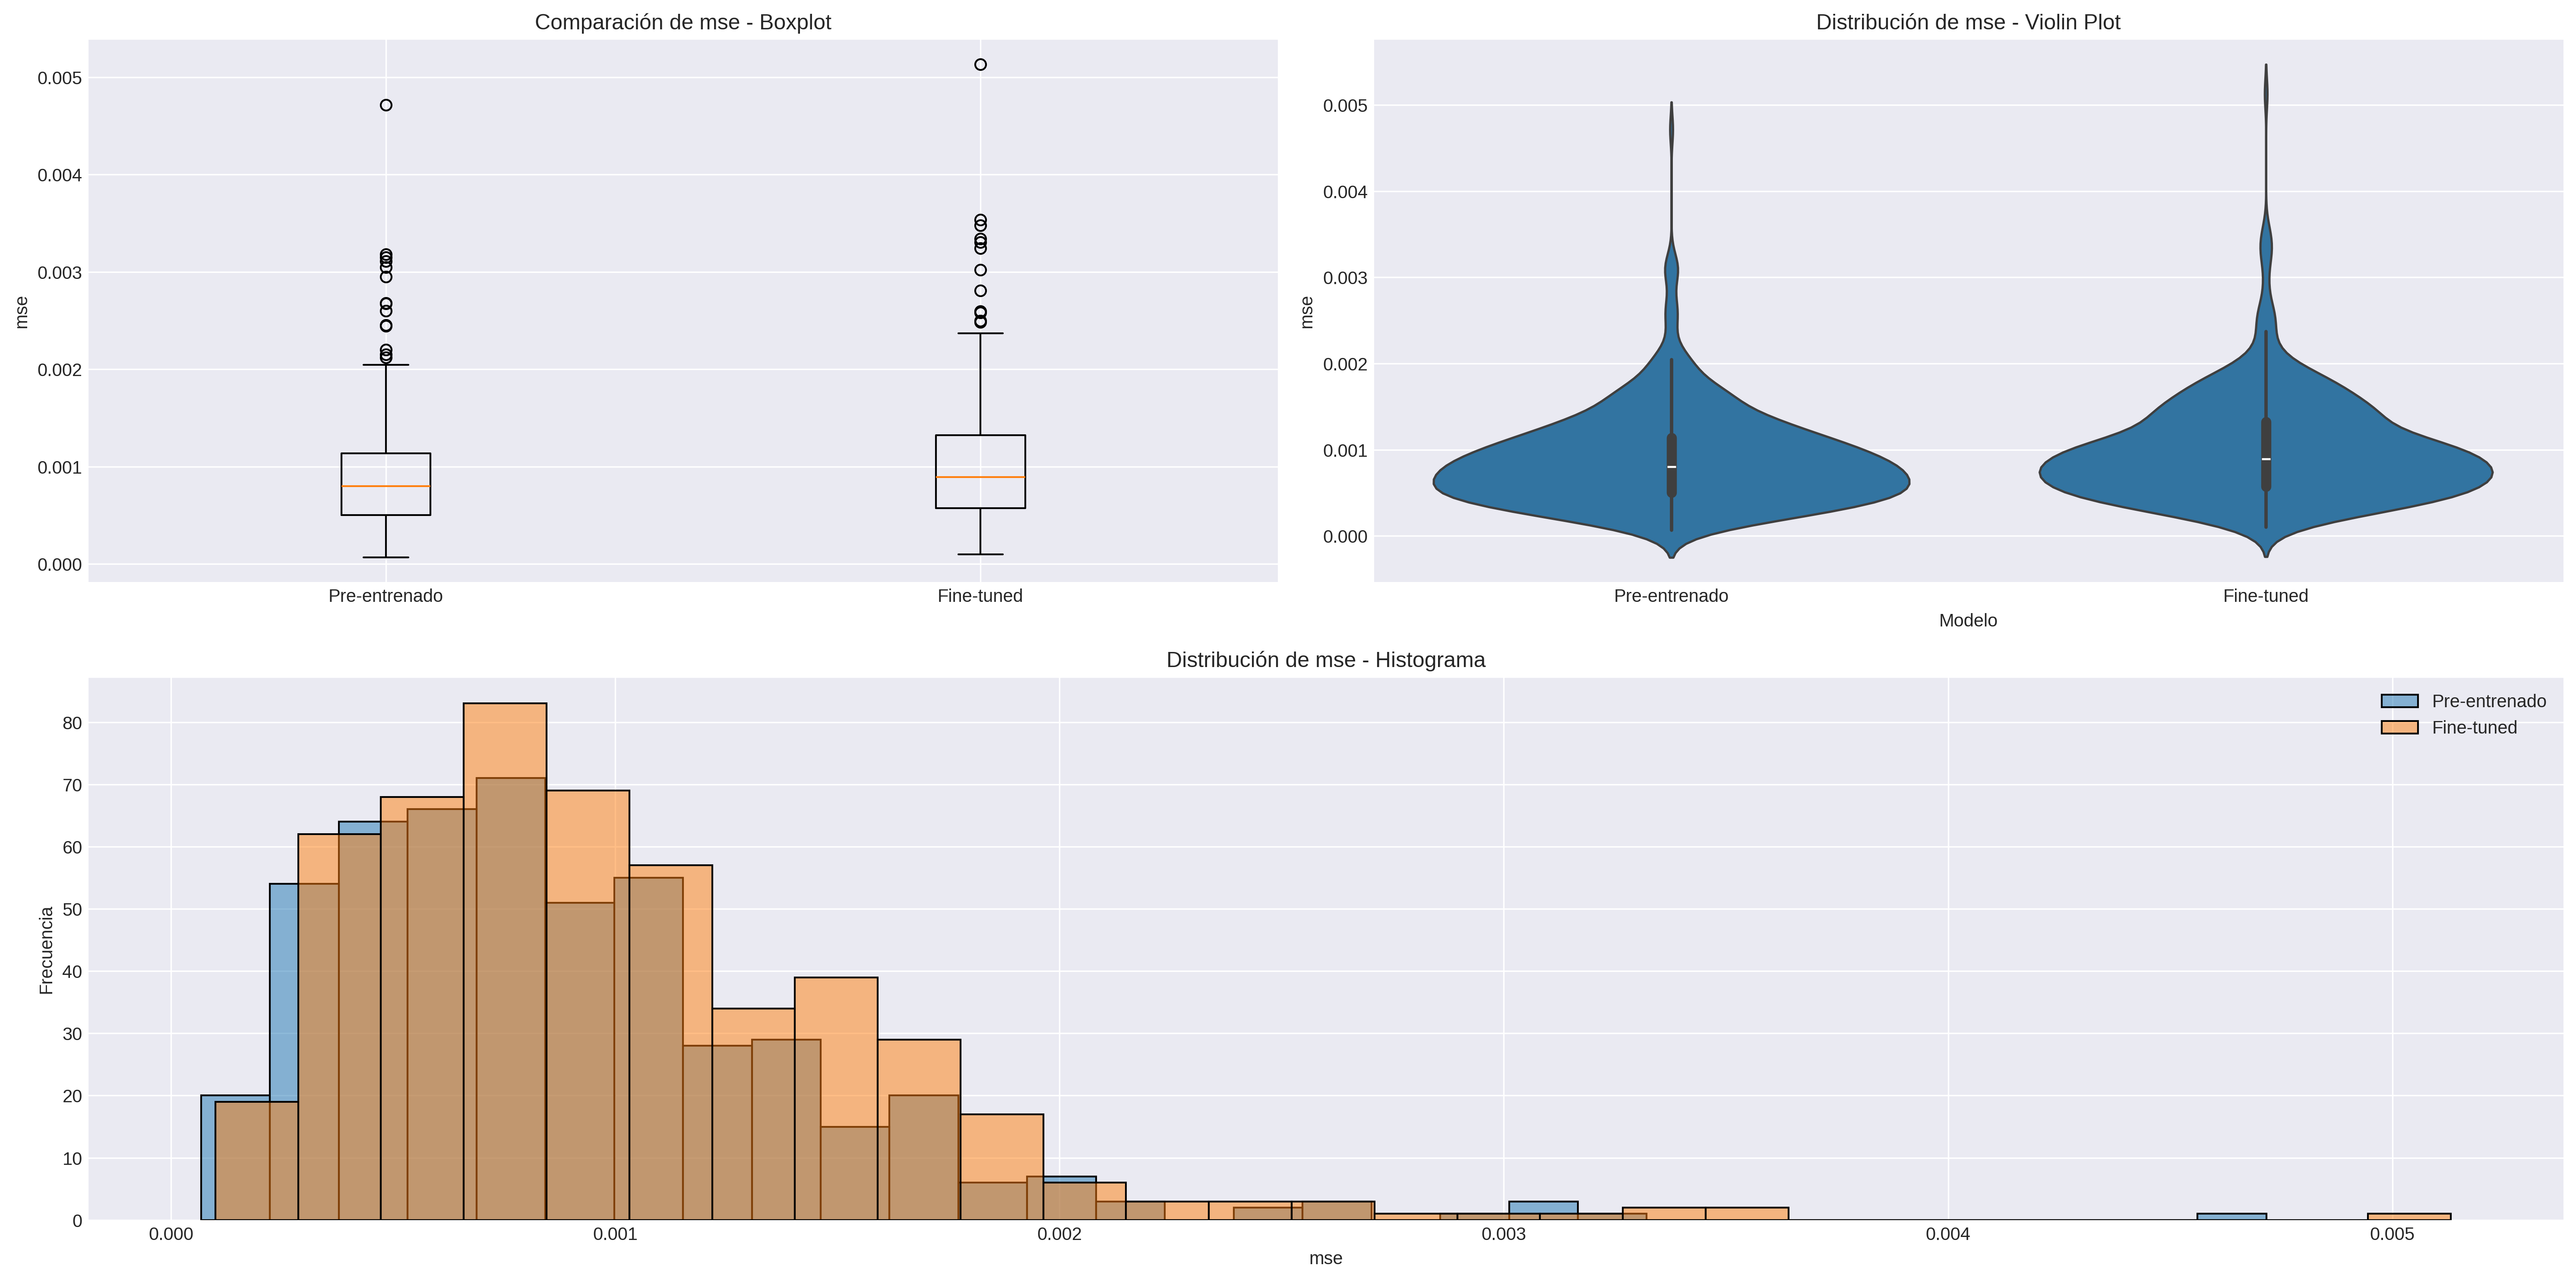
\includegraphics[width=\textwidth]{Images/comparison_plots_mse_no_phy.png}
            \caption{Comparación entre fine-tuning sin componente física y modelo pre-entrenado}
            \label{fig:mse_completo}
        \end{subfigure}
        \hfill
        \begin{subfigure}[b]{0.48\textwidth}
            \centering
            % FT No-Structural vs Baseline
            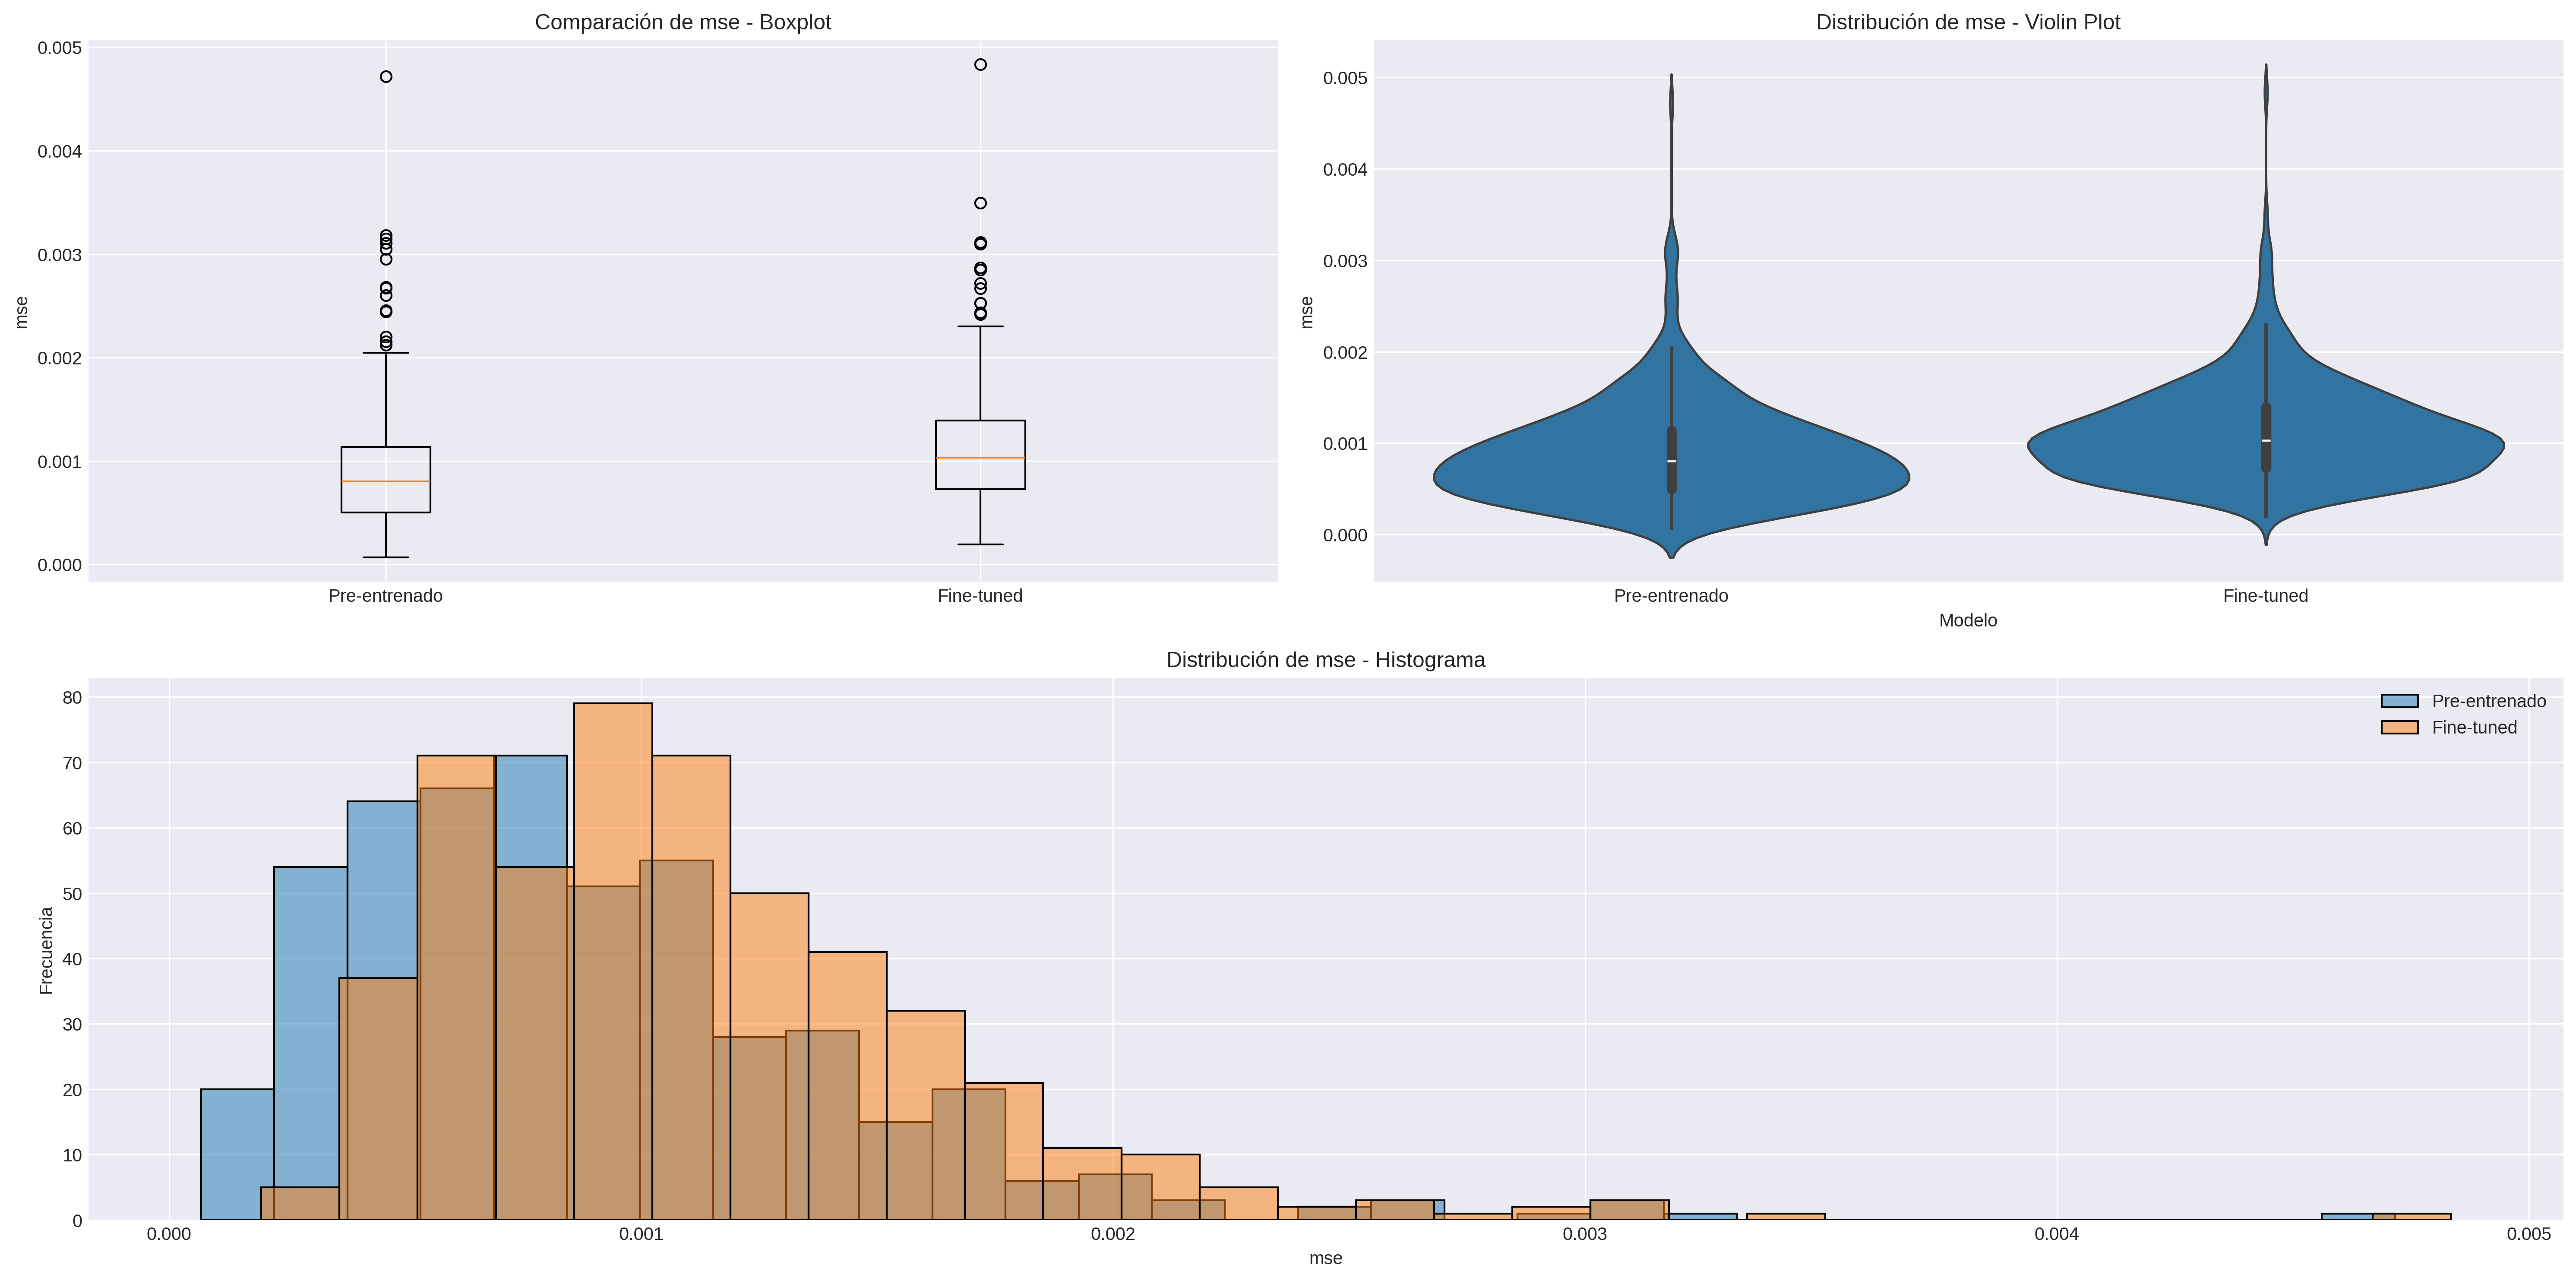
\includegraphics[width=\textwidth]{Images/comparison_plots_mse_no_struct.png}
            \caption{Comparación entre fine-tuning sin componente estructural y modelo pre-entrenado}
            \label{fig:mse_no_struct}
        \end{subfigure}
        
        \vspace{0.5cm}
        
        \begin{subfigure}[b]{0.7\textwidth}
            \centering
            % FT vs Baseline
            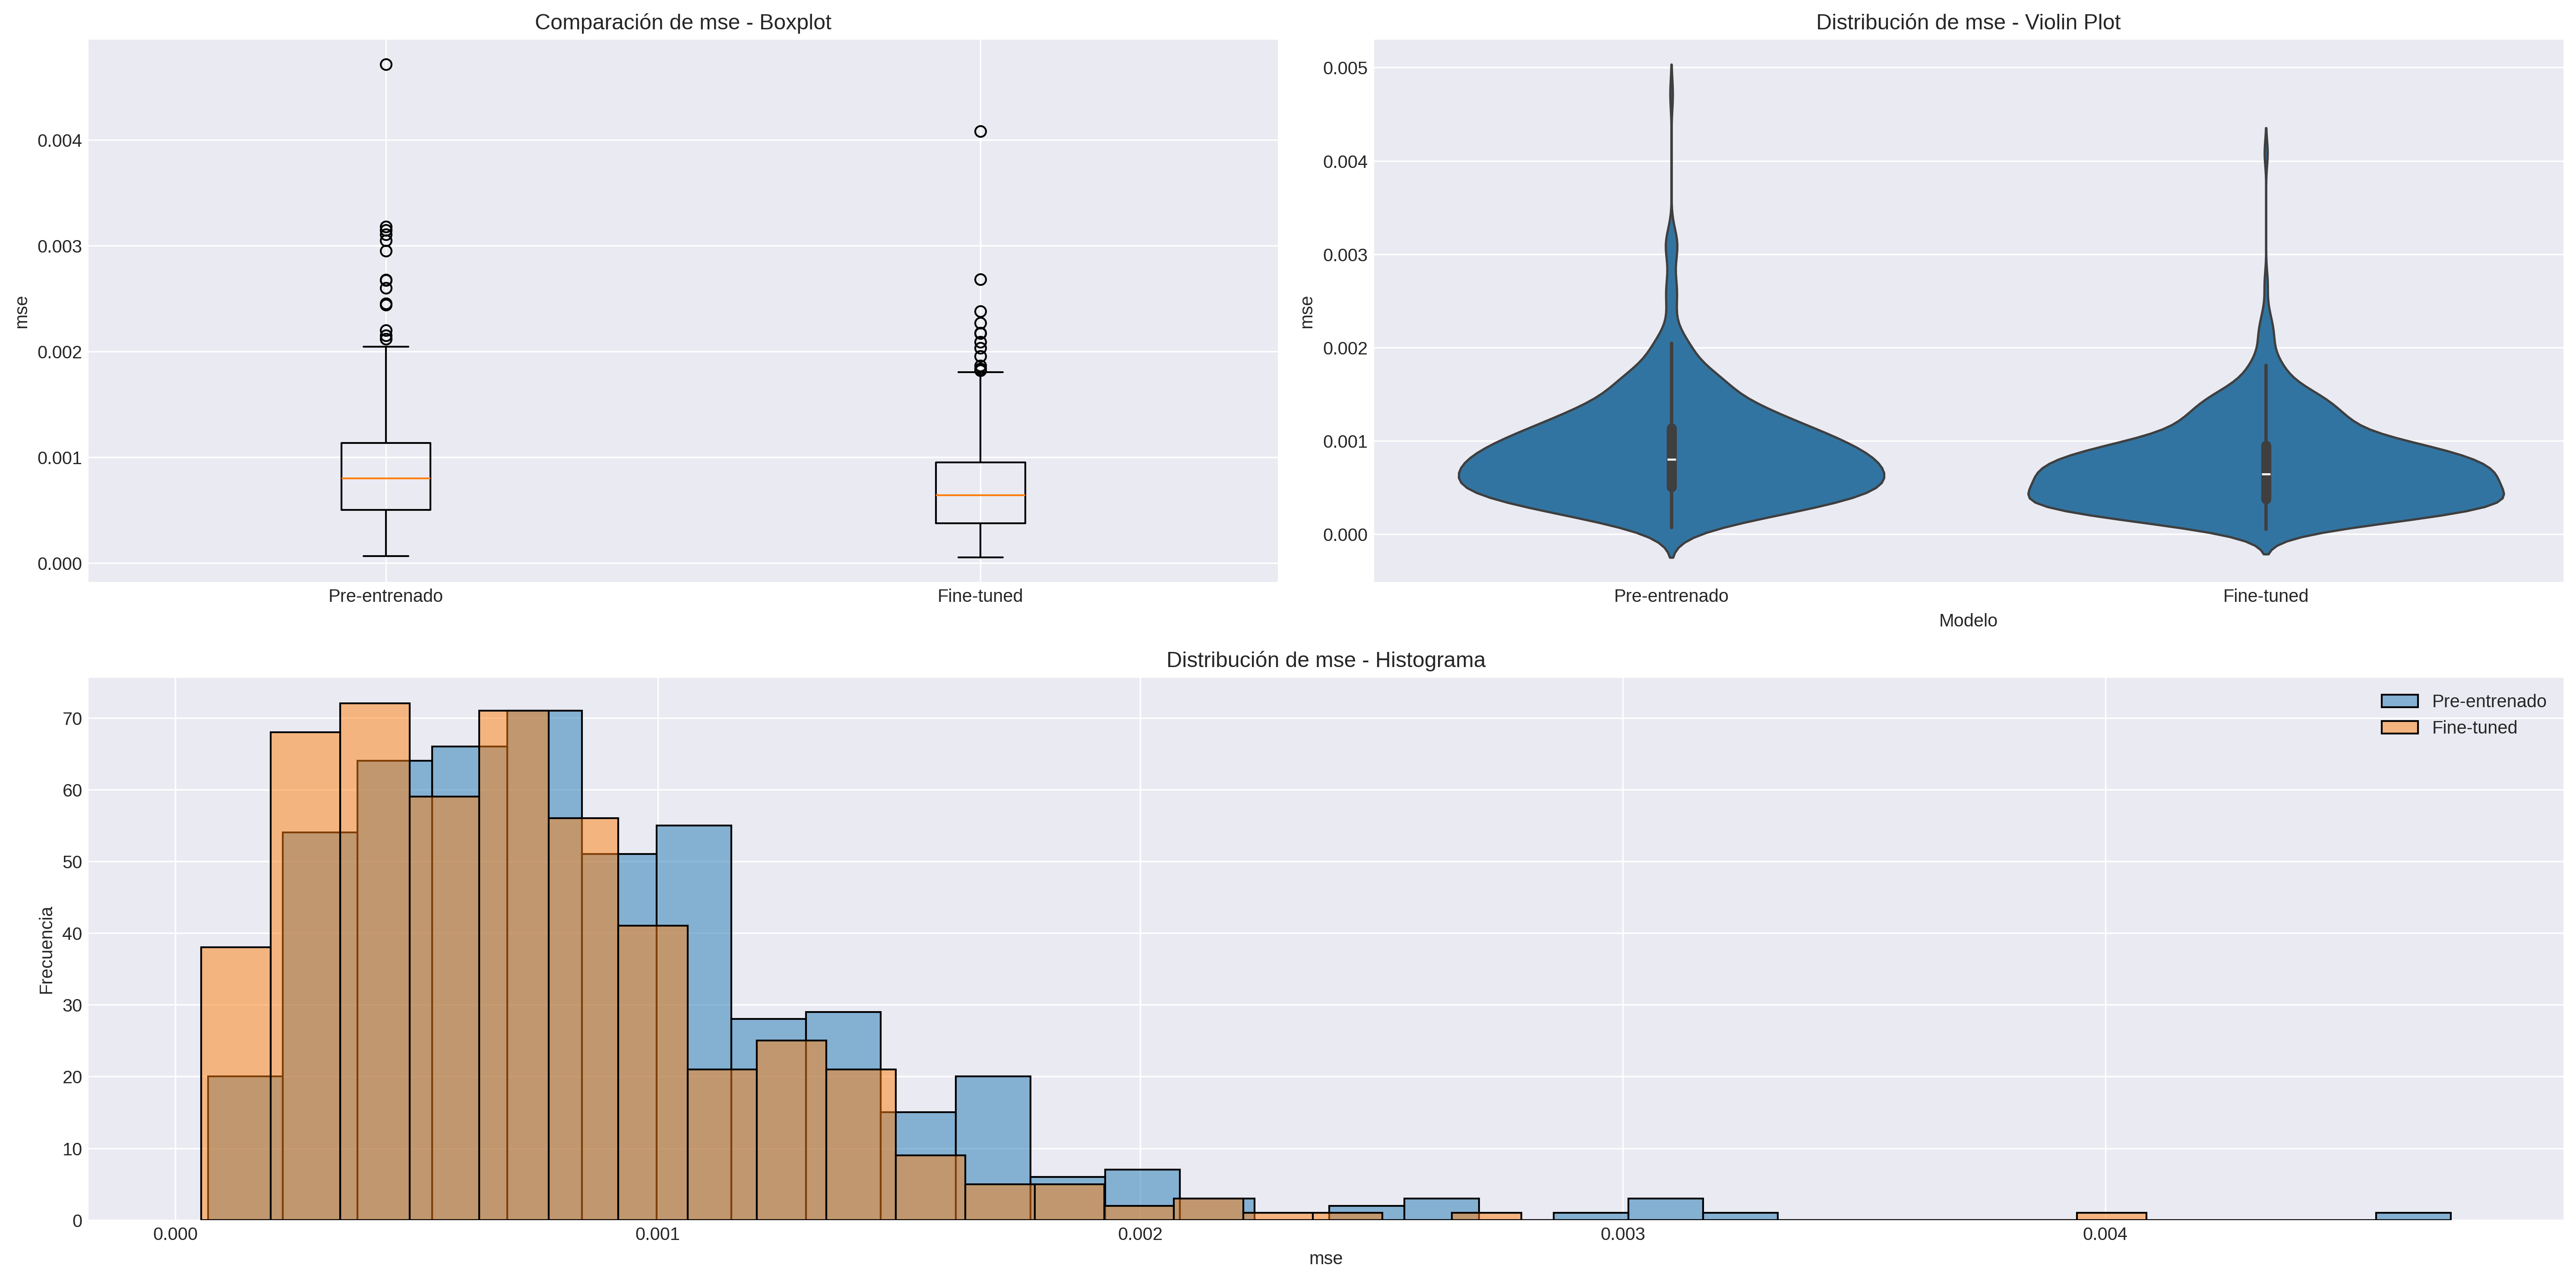
\includegraphics[width=\textwidth]{Images/comparison_plots_mse_sup.png}
            \caption{Comparación entre fine-tuning (FT) completo y modelo pre-entrenado}
            \label{fig:mse_no_phy}
        \end{subfigure}
        
        \caption{Análisis comparativo del Error Cuadrático Medio (MSE) entre el modelo pre-entrenado y las variantes de fine-tuning implementadas. a) Comparación entre fine-tuning sin componente física y modelo pre-entrenado. b) Comparación entre fine-tuning sin componente estructural y modelo pre-entrenado. c) Comparación entre fine-tuning completo y modelo pre-entrenado.}
        \label{fig:mse_analysis}
    \end{figure}
\end{figure}


\paragraph{Fine-tuning Completo (FT)}
El modelo con fine-tuning completo demuestra una mejora sustancial en términos del MSE. El error medio se redujo de $8.91 \times 10^{-4}$ en el modelo pre-entrenado a $7.26 \times 10^{-4}$ en el modelo fine-tuned, representando una mejora del 18.46\%. Esta reducción es particularmente significativa porque el MSE penaliza más severamente los errores grandes, indicando que el fine-tuning no solo mejora el rendimiento promedio sino que también reduce la incidencia de errores de gran magnitud.

La reducción en la variabilidad de los errores se evidencia en la disminución de la desviación estándar de $5.51 \times 10^{-4}$ a $4.64 \times 10^{-4}$. El rango de errores también se contrajo favorablemente, con el valor mínimo mejorando ligeramente de $6.8 \times 10^{-5}$ a $5.4 \times 10^{-5}$ y el máximo reduciéndose de $4.716 \times 10^{-3}$ a $4.086 \times 10^{-3}$. 

El análisis estadístico confirma la significancia de estas mejoras. A pesar de que las pruebas de Shapiro-Wilk ($W = 0.8855$ y $W = 0.8997$, ambas con $p < 0.001$) indican que las distribuciones no siguen una distribución normal, tanto la prueba $t$ pareada ($t = 12.3630$, $p < 0.001$) como la prueba no paramétrica de Wilcoxon ($W = 25146.0000$, $p < 0.001)$ confirman que la diferencia es estadísticamente significativa. El tamaño del efecto ($d$ de $Cohen = 0.3231$) indica una mejora de magnitud media.

\paragraph{Fine-tuning sin Componente Física (FT No-Physical)}
La eliminación de la componente física en el entrenamiento resulta en un deterioro notable del rendimiento. El MSE medio aumentó a $1.004 \times 10^{-3}$, lo que representa un empeoramiento del 12.69\% respecto al modelo pre-entrenado. Este incremento en el error viene acompañado de un aumento en la variabilidad, con una desviación estándar de $5.90 \times 10^{-4}$ y una expansión del rango de errores (mínimo: $1.00 \times 10^{-4}$, máximo: $5.131 \times 10^{-3}$).

Las pruebas estadísticas confirman que este deterioro es significativo, con un estadístico $t$ de $-11.9974$ $(p < 0.001)$ y un estadístico de Wilcoxon $W = 26066.0000$ ($p < 0.001$). El tamaño del efecto ($d$ de $Cohen = -0.1981$) indica que, aunque el impacto es negativo, su magnitud es relativamente pequeña en comparación con otros ablaciones.

\paragraph{Fine-tuning sin Componente Estructural (FT No-Structural)}
La ausencia de la componente estructural produce el deterioro más significativo en términos del MSE. El error medio aumentó a $1.119 \times 10^{-3}$, representando un empeoramiento del 25.69\% respecto al modelo pre-entrenado. Este incremento sustancial en el MSE es particularmente preocupante dado que indica un aumento en la frecuencia y magnitud de los errores grandes de reconstrucción.

La distribución de errores muestra un desplazamiento sistemático hacia valores más altos, con un valor mínimo de $1.95 \times 10^{-4}$ y un máximo de $4.834 \times 10^{-3}$. El análisis estadístico confirma la gravedad de este deterioro, con un estadístico $t$ de $-21.1018$ $(p < 0.001)$ y un estadístico de Wilcoxon $W = 10718.0000$ $(p < 0.001)$. El tamaño del efecto ($d$ de $Cohen = -0.4220$) indica un impacto negativo de magnitud media, subrayando la importancia crítica de la componente estructural en la función de pérdida.

Este análisis del MSE refuerza las conclusiones obtenidas del MAE, demostrando que la eliminación de cualquier componente de la función de pérdida resulta en un deterioro significativo del rendimiento, siendo la componente estructural particularmente crucial para mantener la calidad de la reconstrucción.

\subsubsection{Error Relativo Medio Normalizado (NRMSE)}


El Error Cuadrático Medio Normalizado (NRMSE) proporciona una medida del error que es independiente de la escala de los datos, facilitando la comparación entre diferentes conjuntos de datos o variables. Al normalizar el error, esta métrica nos permite evaluar la calidad relativa de la reconstrucción en términos porcentuales respecto a la magnitud de los datos originales.


\begin{figure}[H]
    \centering
    \begin{subfigure}[b]{0.48\textwidth}
        \centering
        % FT No-Physical vs Baseline
        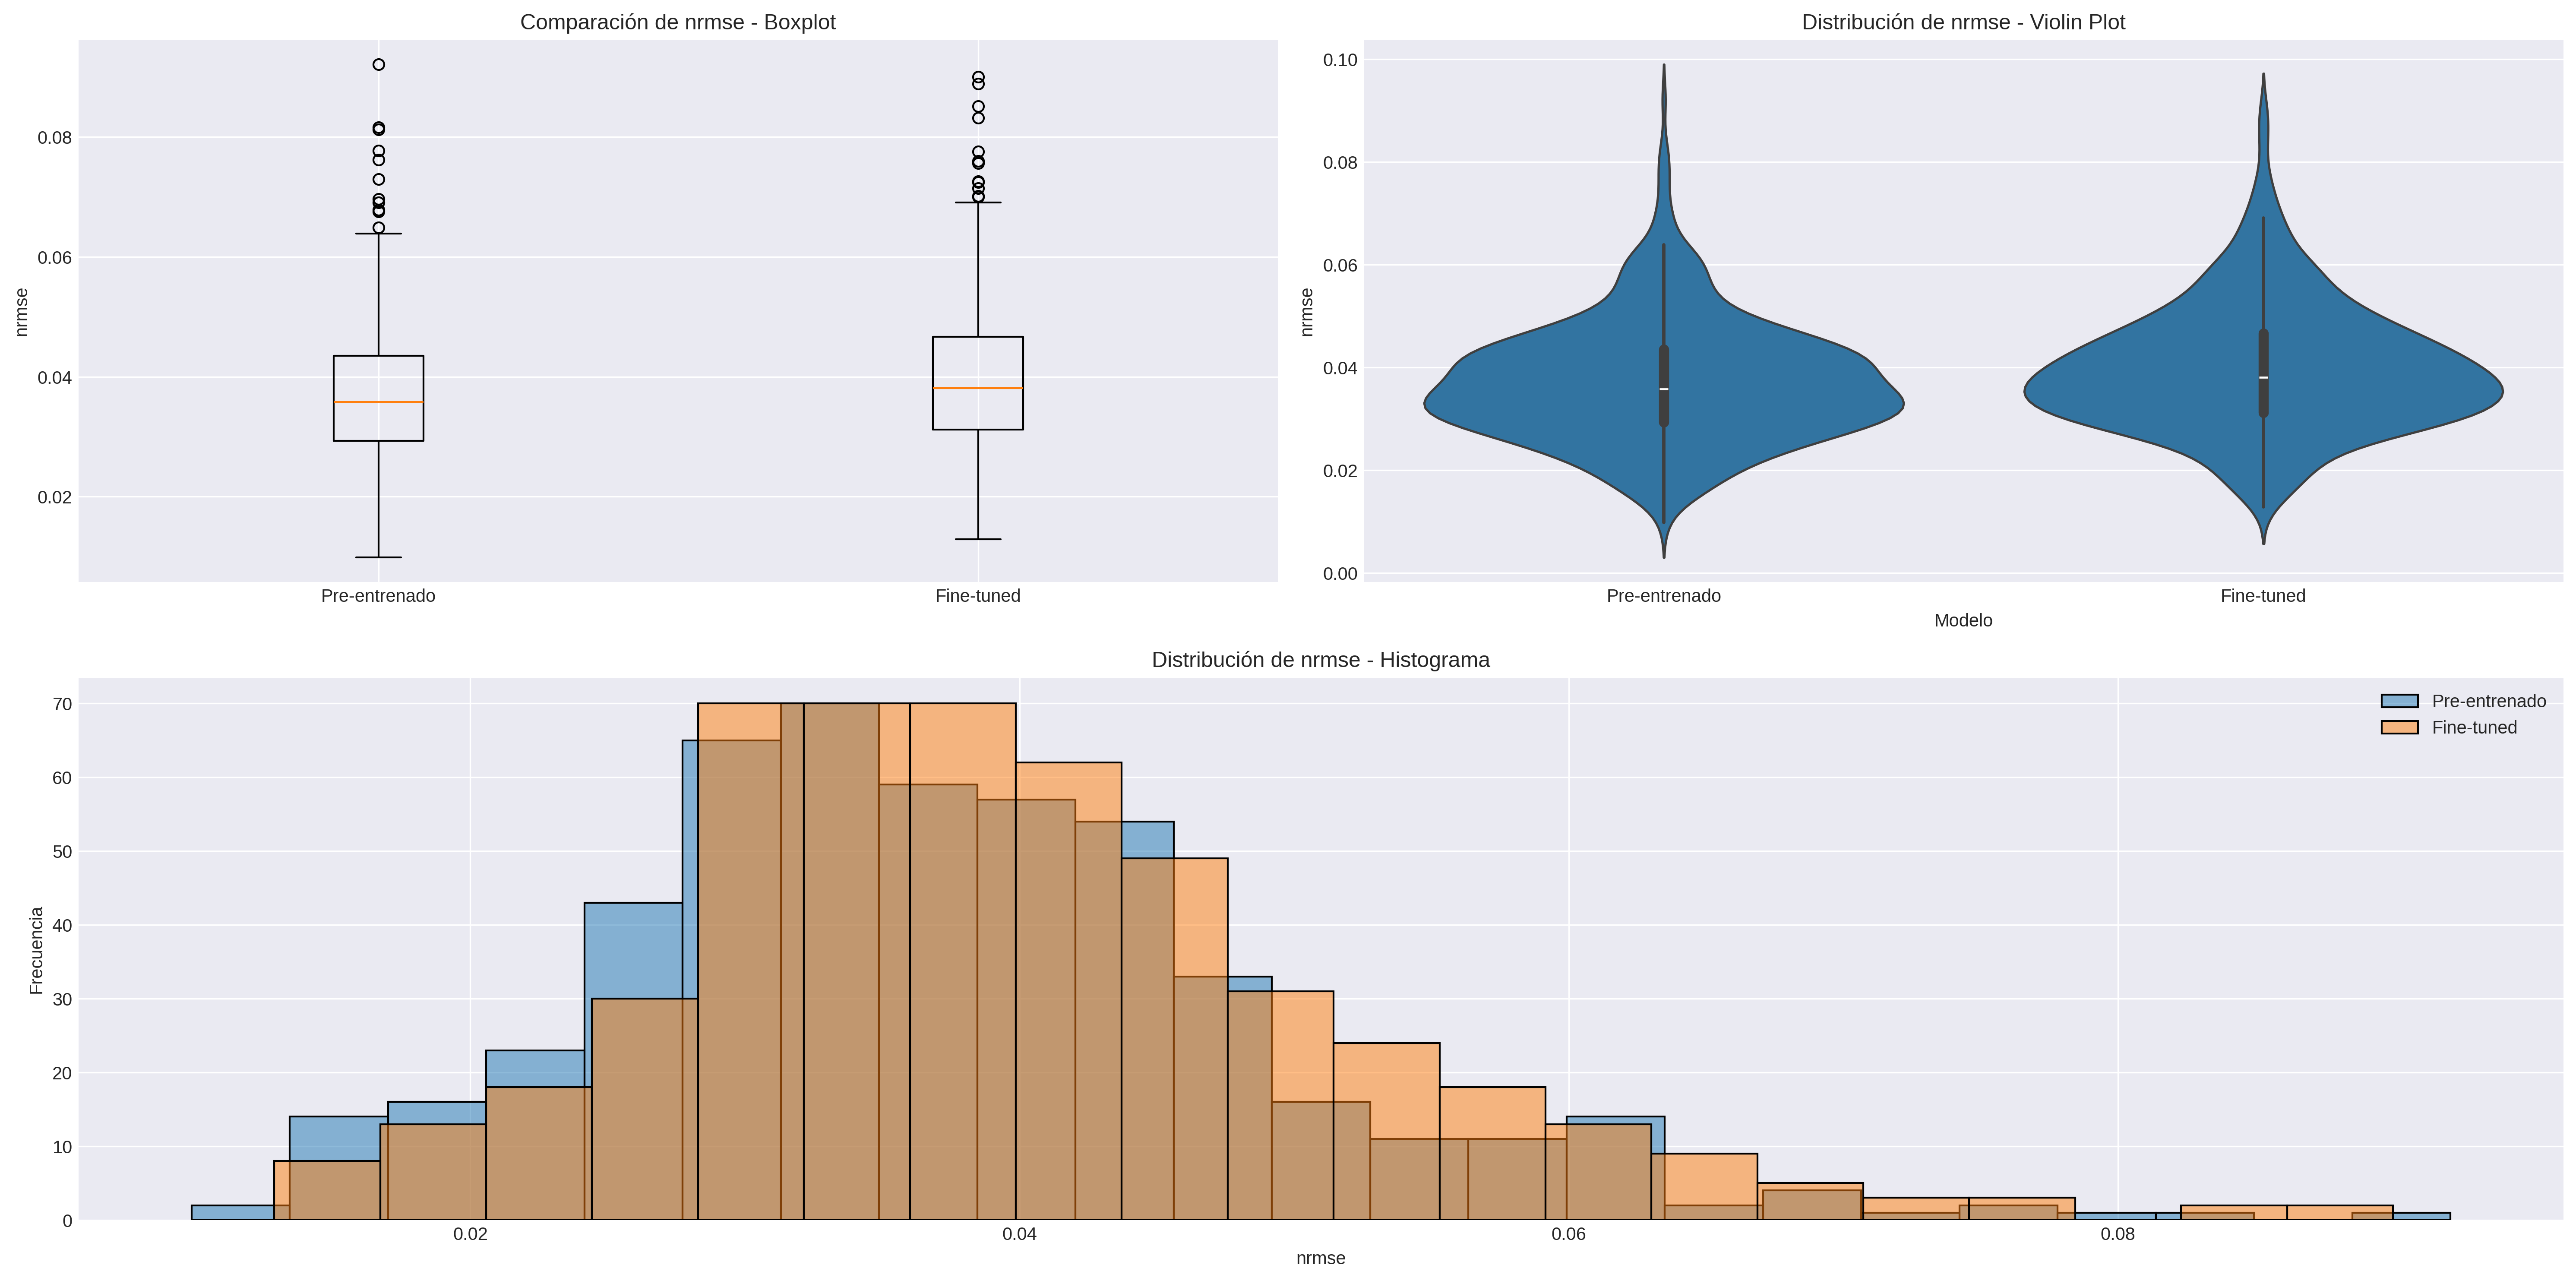
\includegraphics[width=\textwidth]{Images/comparison_plots_nrmse_no_phy.png}
        \caption{Comparación entre fine-tuning sin componente física y modelo pre-entrenado}
        \label{fig:nrmse_hist}
    \end{subfigure}
    \hfill
    \begin{subfigure}[b]{0.48\textwidth}
        \centering
        % FT No-Structural vs Baseline
        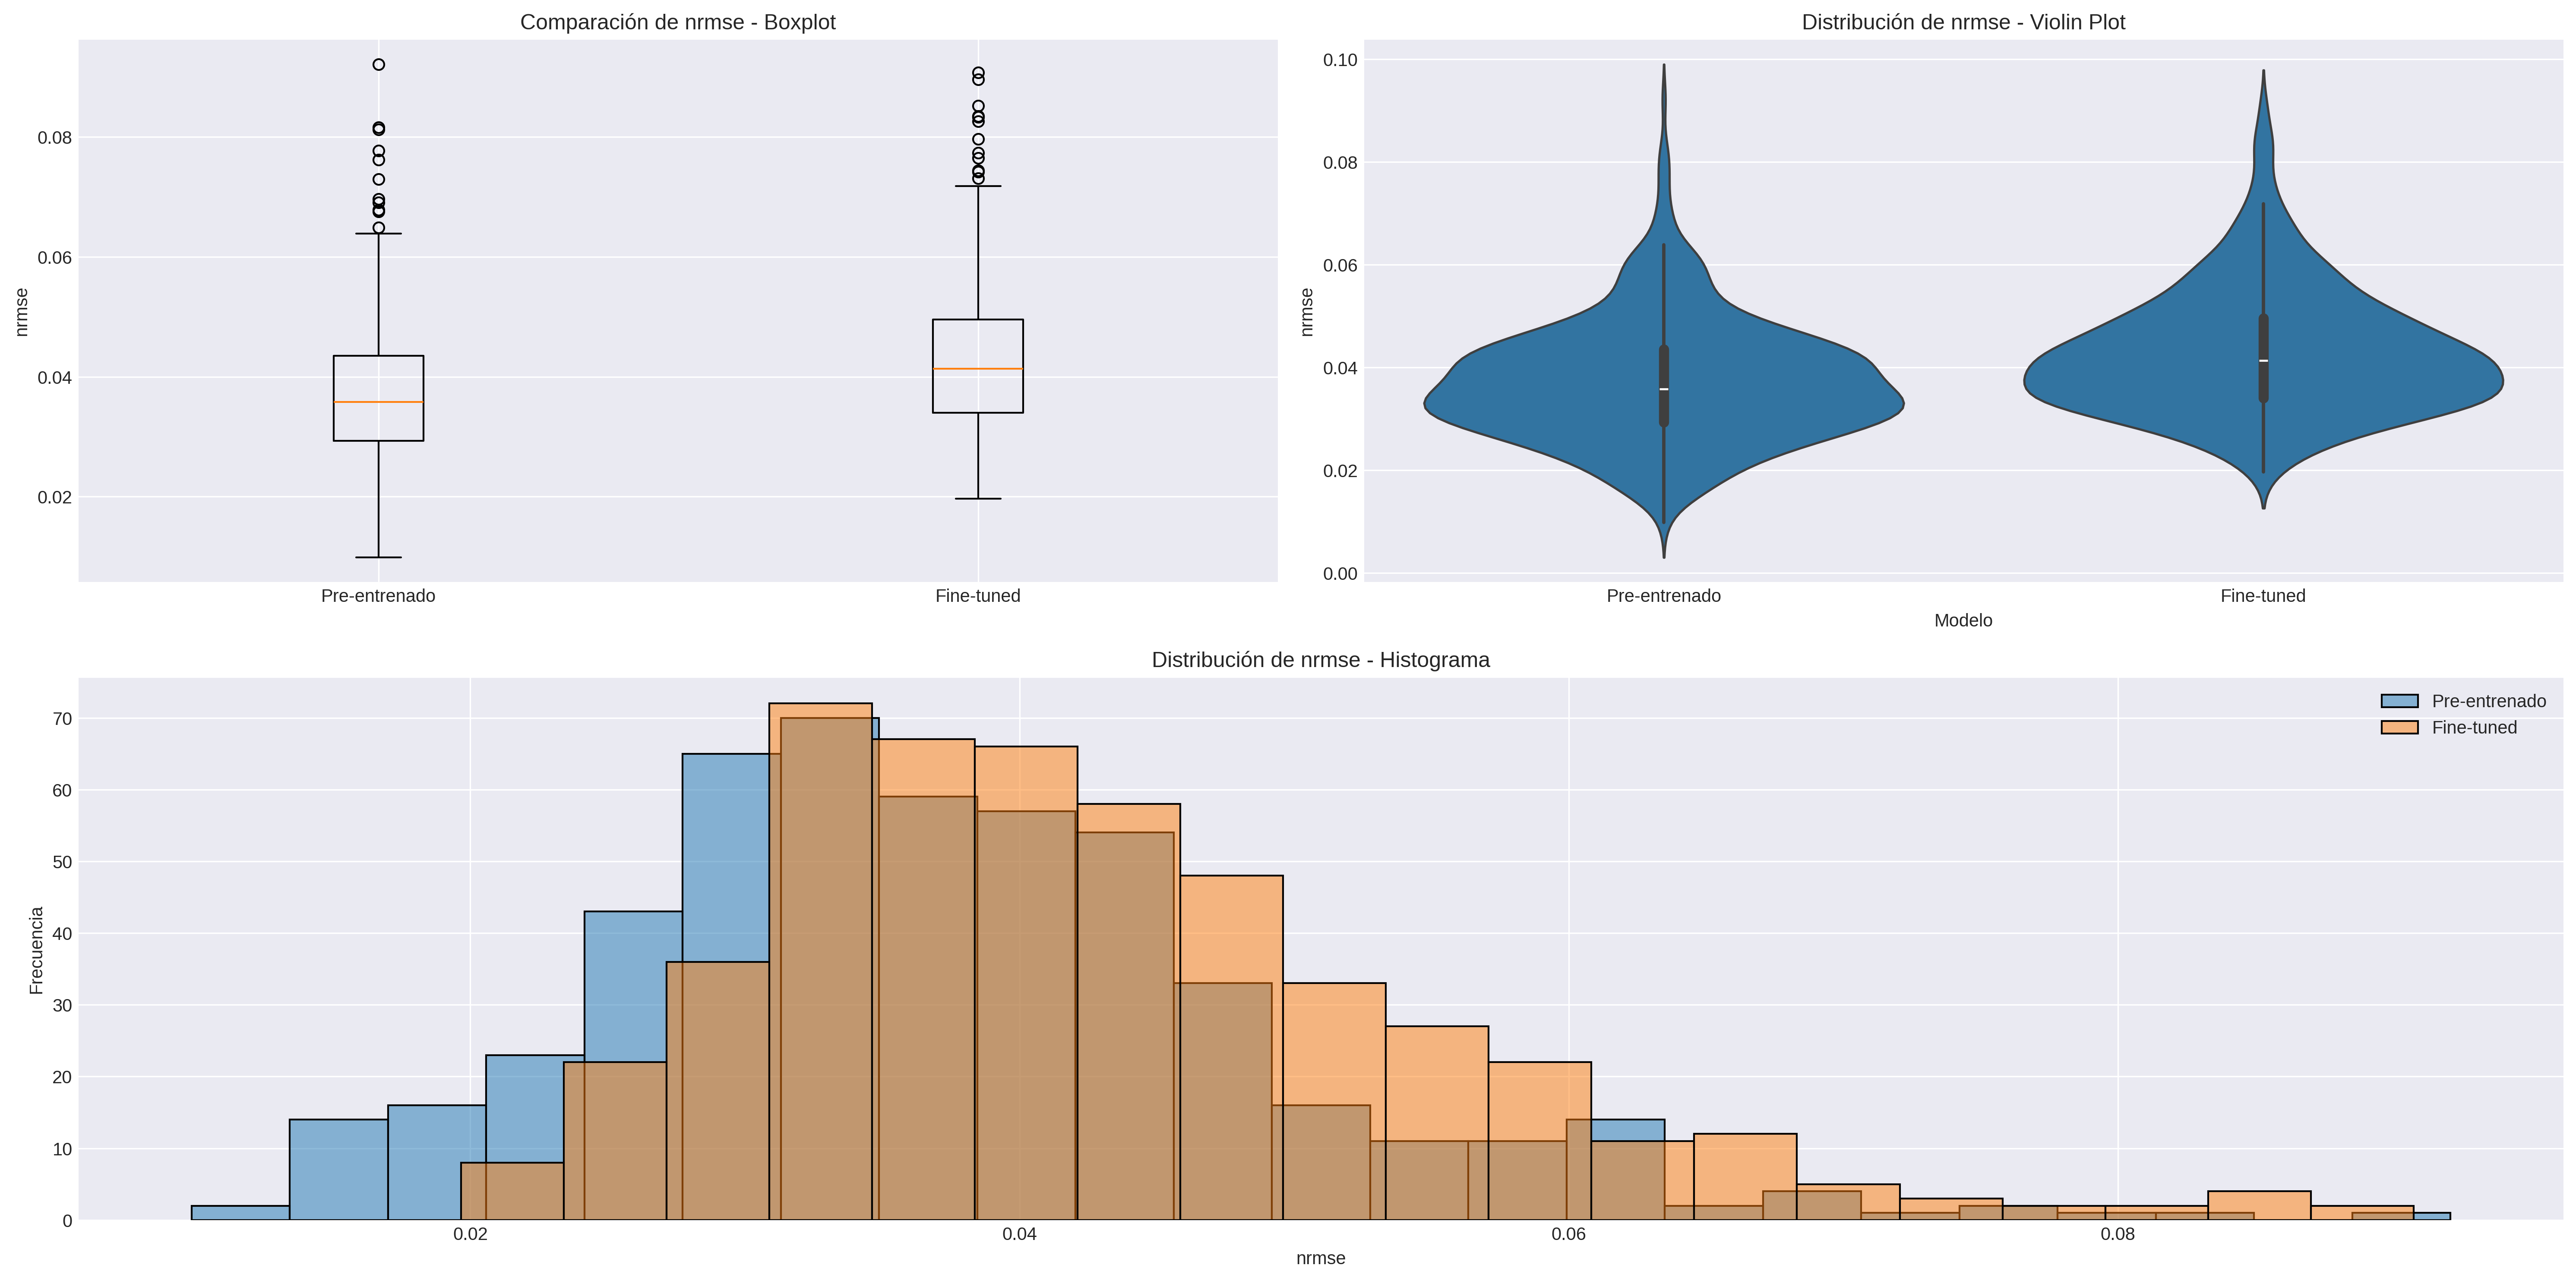
\includegraphics[width=\textwidth]{Images/comparison_plots_nrmse_no_struct.png}
        \caption{Comparación entre fine-tuning sin componente estructural y modelo pre-entrenado}
        \label{fig:nrmse_violin}
    \end{subfigure}
    
    \vspace{0.5cm}
    
    \begin{subfigure}[b]{0.7\textwidth}
        \centering
        % FT vs Baseline
        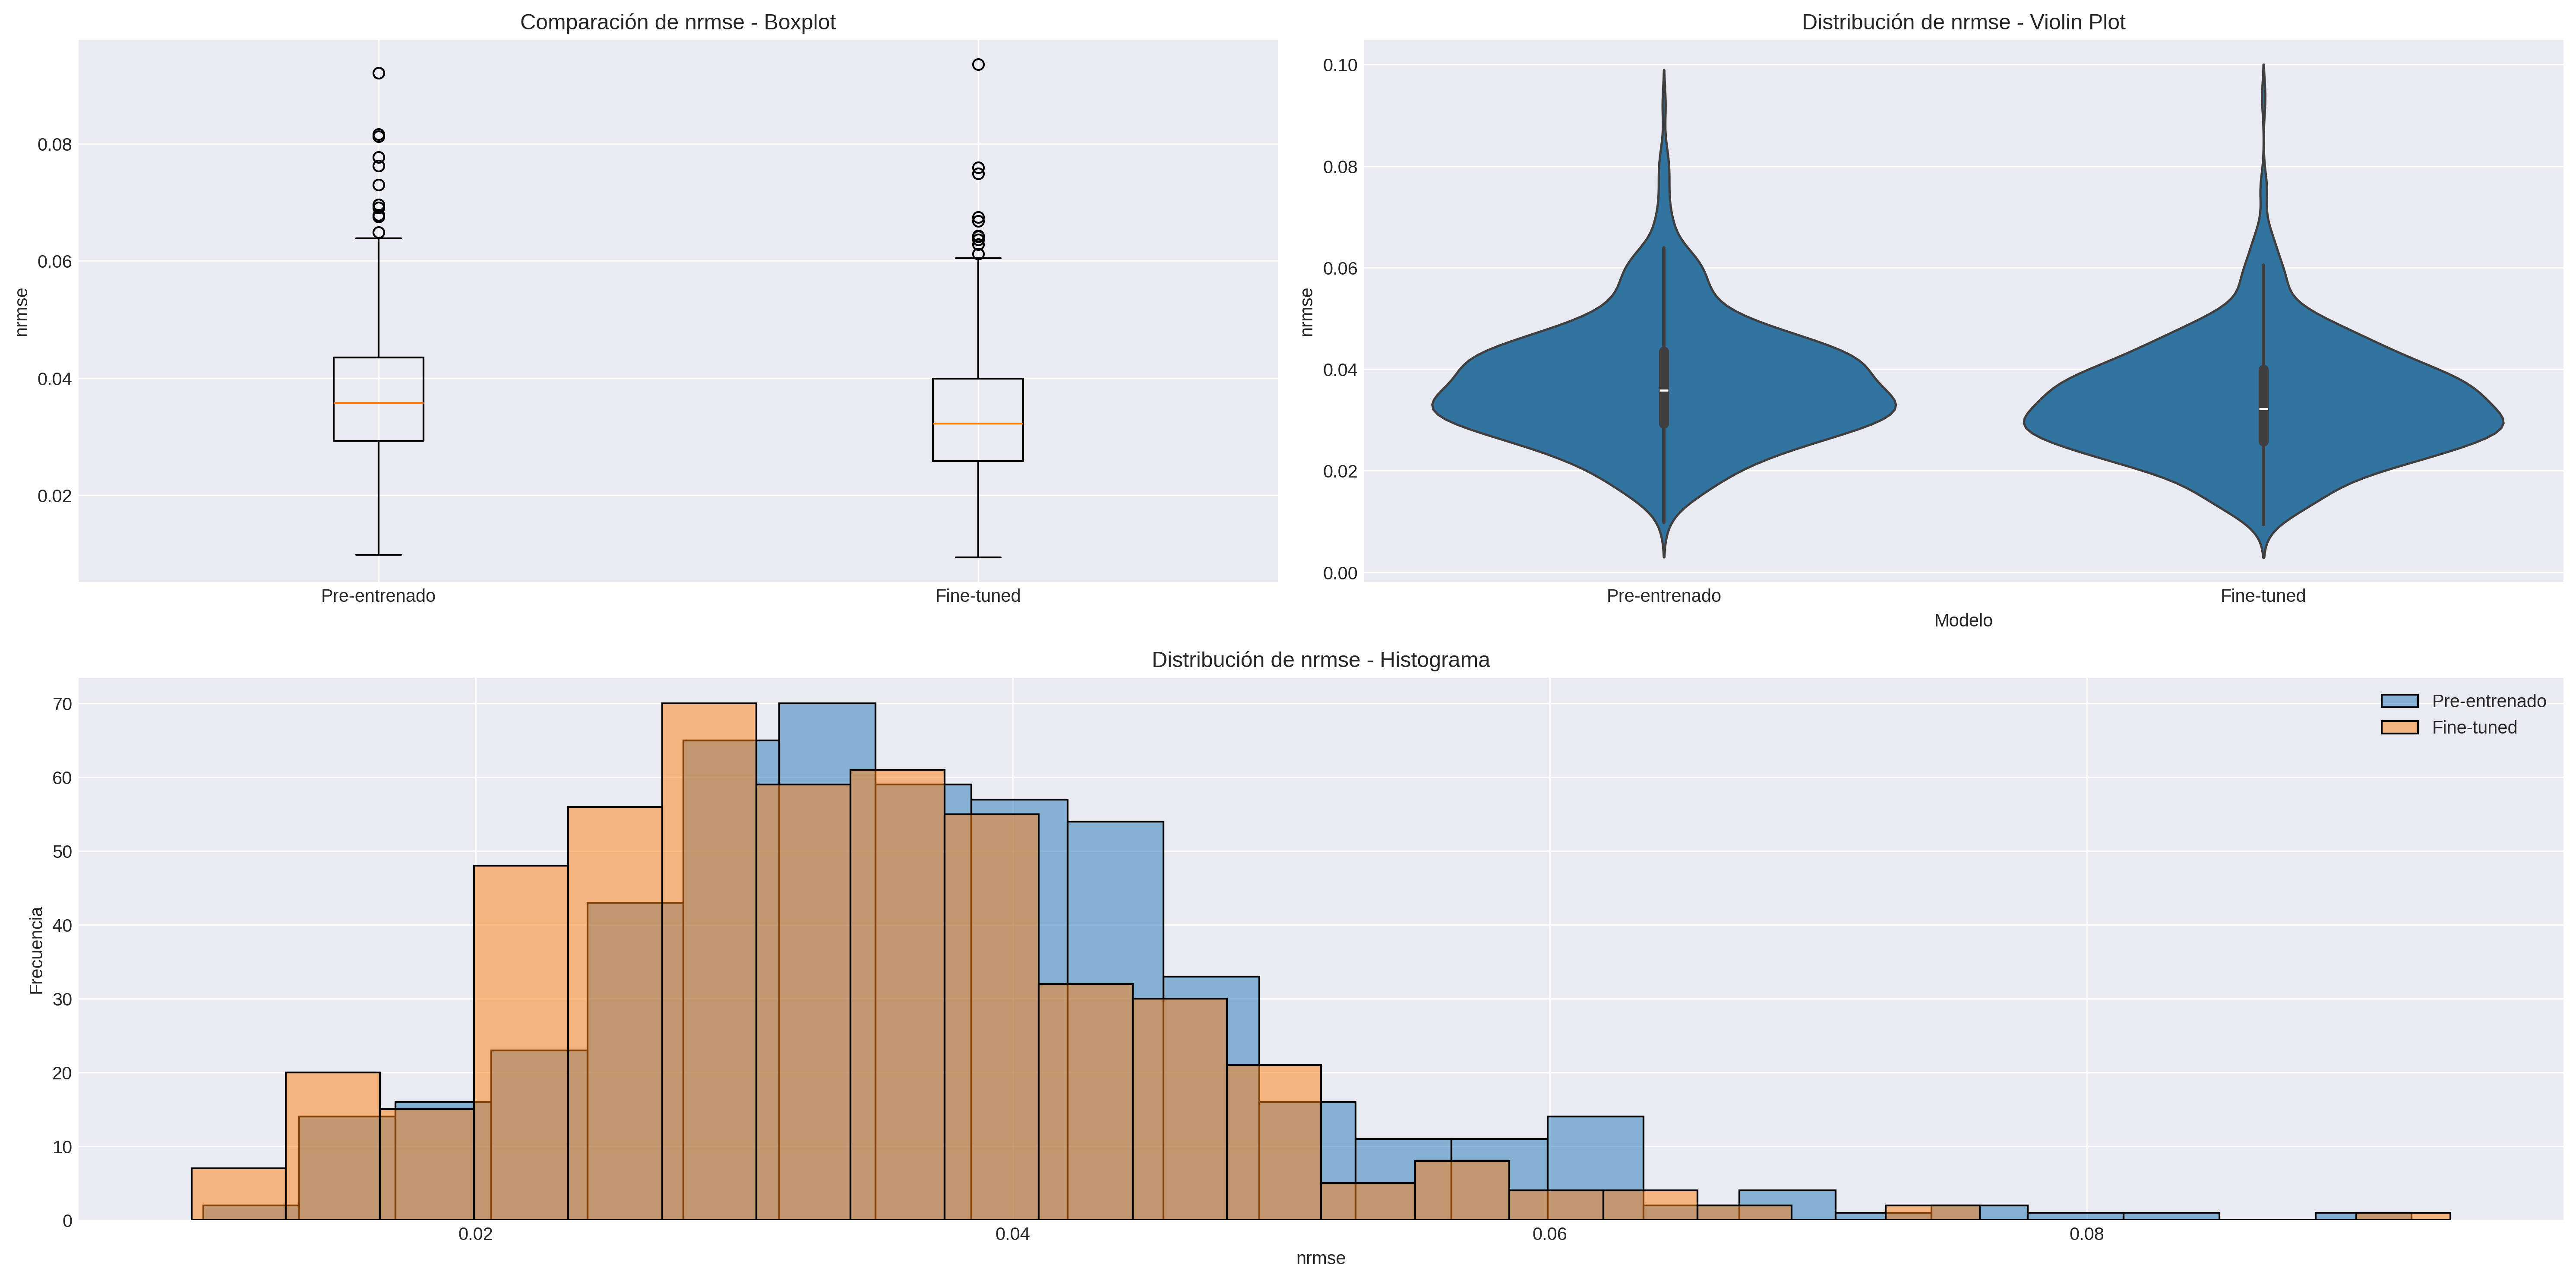
\includegraphics[width=\textwidth]{Images/comparison_plots_nrmse_sup.png}
        \caption{Comparación entre fine-tuning (FT) completo y modelo pre-entrenado}
        \label{fig:nrmse_box}
    \end{subfigure}
    
    \caption{Análisis comparativo del Error Relativo Medio Normalizado (NRMSE) entre el modelo pre-entrenado y las variantes de fine-tuning implementadas. a) Comparación entre fine-tuning sin componente física y modelo pre-entrenado. b) Comparación entre fine-tuning sin componente estructural y modelo pre-entrenado. c) Comparación entre fine-tuning completo y modelo pre-entrenado.}
    \label{fig:nrmse_analysis}
\end{figure}



\paragraph{Fine-tuning Completo (FT)}
El modelo con fine-tuning completo demuestra una mejora significativa en la precisión de reconstrucción normalizada. El NRMSE medio se redujo de 0.037209 (3.72\%) en el modelo pre-entrenado a 0.033431 (3.34\%) en el modelo fine-tuned, representando una mejora del 10.15\%. Esta reducción es particularmente relevante porque indica que el modelo mejoró su capacidad de reconstrucción de manera consistente a través de diferentes escalas de magnitud en los datos.

La consistencia de la mejora se refleja en la reducción de la variabilidad, con una disminución en la desviación estándar de 0.011857 a 0.011228. El rango de errores también muestra una mejora, con el valor mínimo reduciéndose de 0.009851 (0.99\%) a 0.009414 (0.94\%). El análisis estadístico confirma la significancia de estas mejoras a través de múltiples pruebas:

\begin{itemize}
    \item La prueba t pareada ($t = 13.3137$, $p < 0.001$) y la prueba de Wilcoxon ($W = 24360.0000$, $p < 0.001$) confirman que la diferencia es estadísticamente significativa
    \item El tamaño del efecto ($d$ de $Cohen = 0.3272$) indica una mejora de magnitud media
    \item Las pruebas de Shapiro-Wilk ($W \approx 0.966$ para ambas distribuciones, $p < 0.001$) sugieren que el análisis no paramétrico es particularmente relevante
\end{itemize}

\paragraph{Fine-tuning sin Componente Física (FT No-Physical)}
La eliminación de la componente física resulta en un deterioro notable del rendimiento normalizado. El NRMSE medio aumentó a 0.039862 (3.99\%), representando un empeoramiento del 7.13\% respecto al modelo pre-entrenado. Este incremento en el error normalizado sugiere que la ausencia de la componente física afecta la capacidad del modelo para capturar las relaciones subyacentes en los datos, independientemente de su escala.

La distribución de errores muestra un desplazamiento sistemático hacia valores más altos, con:

\begin{itemize}
    \item Un incremento en el valor mínimo a 0.012861 (1.29\%)
    \item Un aumento en la variabilidad (desviación estándar de 0.012413)
    \item Una modificación en la forma de la distribución, como lo indica la prueba de Shapiro-Wilk ($W = 0.9647$, $p < 0.001$)
\end{itemize}

El análisis estadístico confirma que este deterioro es significativo ($t = -12.3593$, $p < 0.001$; $W = 25214.0000$, $p < 0.001$), aunque el tamaño del efecto ($d$ de $Cohen = -0.2186$) sugiere que el impacto, aunque negativo, es relativamente moderado.

\paragraph{Fine-tuning sin Componente Estructural (FT No-Structural)}
La ausencia de la componente estructural produce el deterioro más significativo en términos del NRMSE. El error medio aumentó a 0.042954 (4.30\%), lo que representa un empeoramiento del 15.44\% respecto al modelo pre-entrenado. Este incremento sustancial en el NRMSE es particularmente revelador porque indica que la componente estructural es fundamental para mantener la precisión de reconstrucción a través de diferentes escalas de magnitud.

El impacto negativo se manifiesta en múltiples aspectos:

\begin{itemize}
    \item Un aumento significativo en el valor mínimo del error a 0.019659 (1.97\%)
    \item Un incremento en la variabilidad (desviación estándar de 0.012241)
    \item Una alteración más pronunciada en la forma de la distribución ($W = 0.9475$, $p < 0.001$)
\end{itemize}

La significancia estadística de este deterioro se confirma mediante múltiples pruebas:

\begin{itemize}
    \item La prueba t pareada muestra un efecto fuerte ($t = -20.0658$, $p < 0.001$)
    \item La prueba de Wilcoxon corrobora estos resultados ($W = 9258.0000$, $p < 0.001$)
    \item El tamaño del efecto ($d$ de $Cohen = -0.4767$) indica un impacto negativo de magnitud media a grande
\end{itemize}

Este análisis del NRMSE complementa y refuerza las conclusiones obtenidas del MSE y MAE, proporcionando una perspectiva normalizada que demuestra cómo los componentes de la función de pérdida afectan la calidad de reconstrucción independientemente de la escala de los datos. La componente estructural se revela nuevamente como el elemento más crítico para mantener la precisión de la reconstrucción.




\subsubsection{Peak Signal-to-Noise Ratio (PSNR)}

El Peak Signal-to-Noise Ratio (PSNR) es una métrica logarítmica que evalúa la calidad de la reconstrucción en términos de la relación entre la máxima señal posible y el ruido introducido por el proceso de reconstrucción. A diferencia de las métricas anteriores, un valor más alto de PSNR indica una mejor calidad de reconstrucción, ya que representa una mejor relación señal-ruido.


\begin{figure}[H]
    \centering
    \begin{subfigure}[b]{0.48\textwidth}
        \centering
        % FT No-Physical vs Baseline
        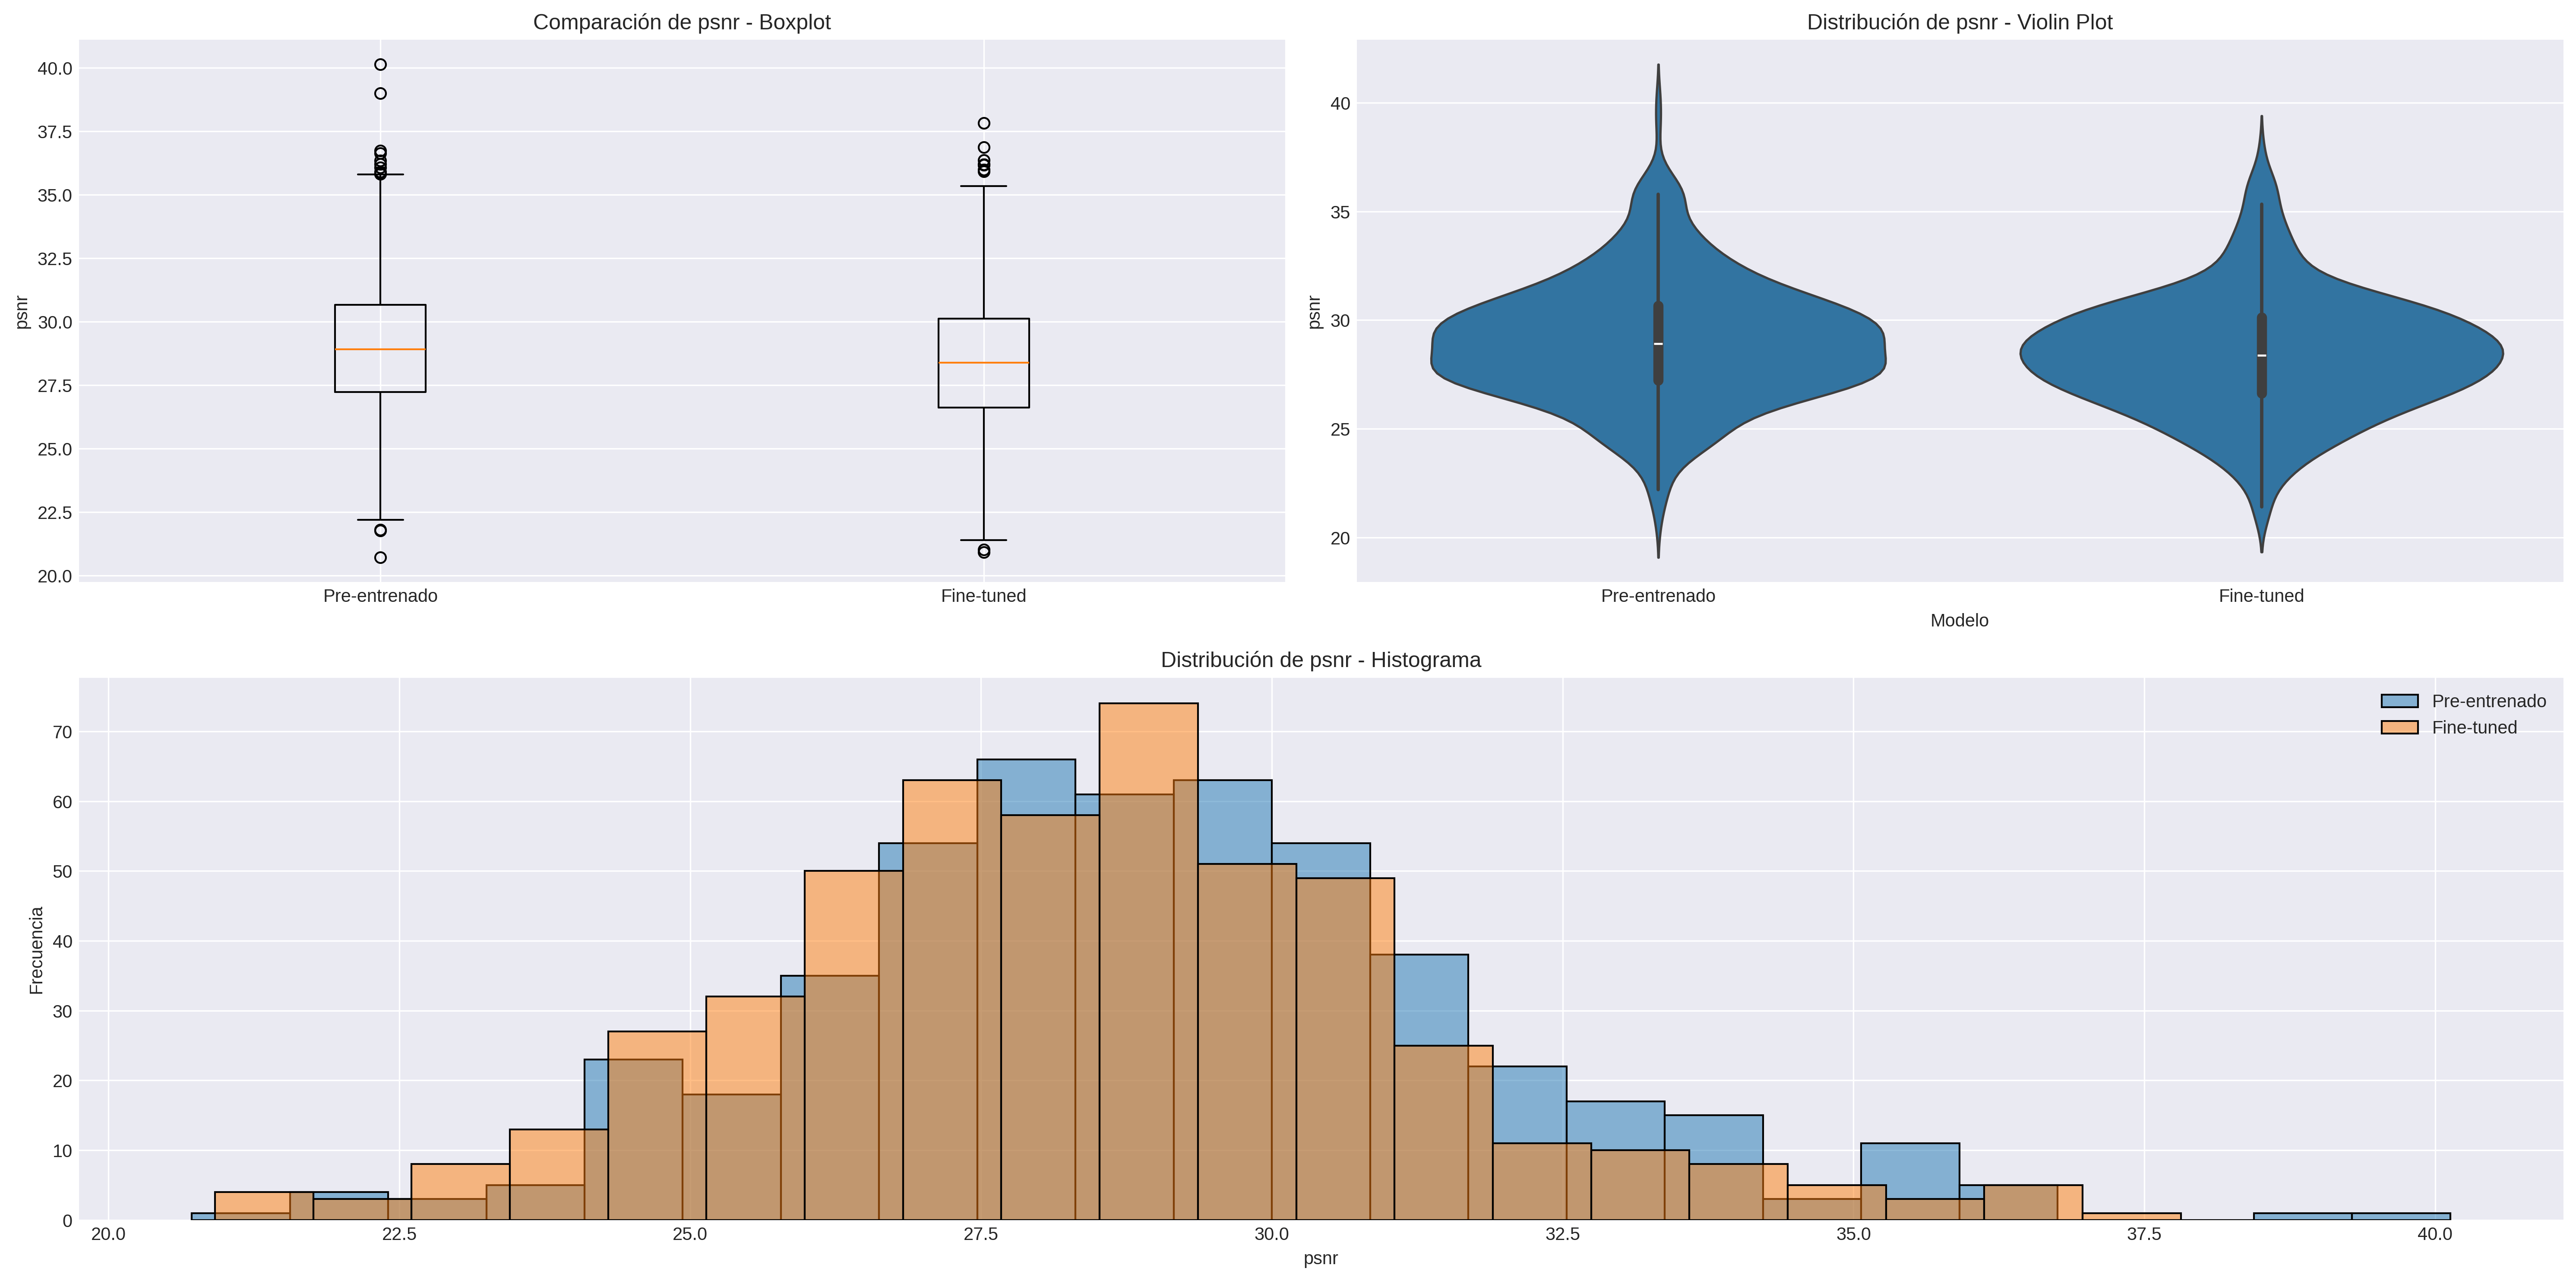
\includegraphics[width=\textwidth]{Images/comparison_plots_psnr_no_phy.png}
        \caption{Comparación entre fine-tuning sin componente física y modelo pre-entrenado}
        \label{fig:psnr_hist}
    \end{subfigure}
    \hfill
    \begin{subfigure}[b]{0.48\textwidth}
        \centering
        % FT No-Structural vs Baseline
        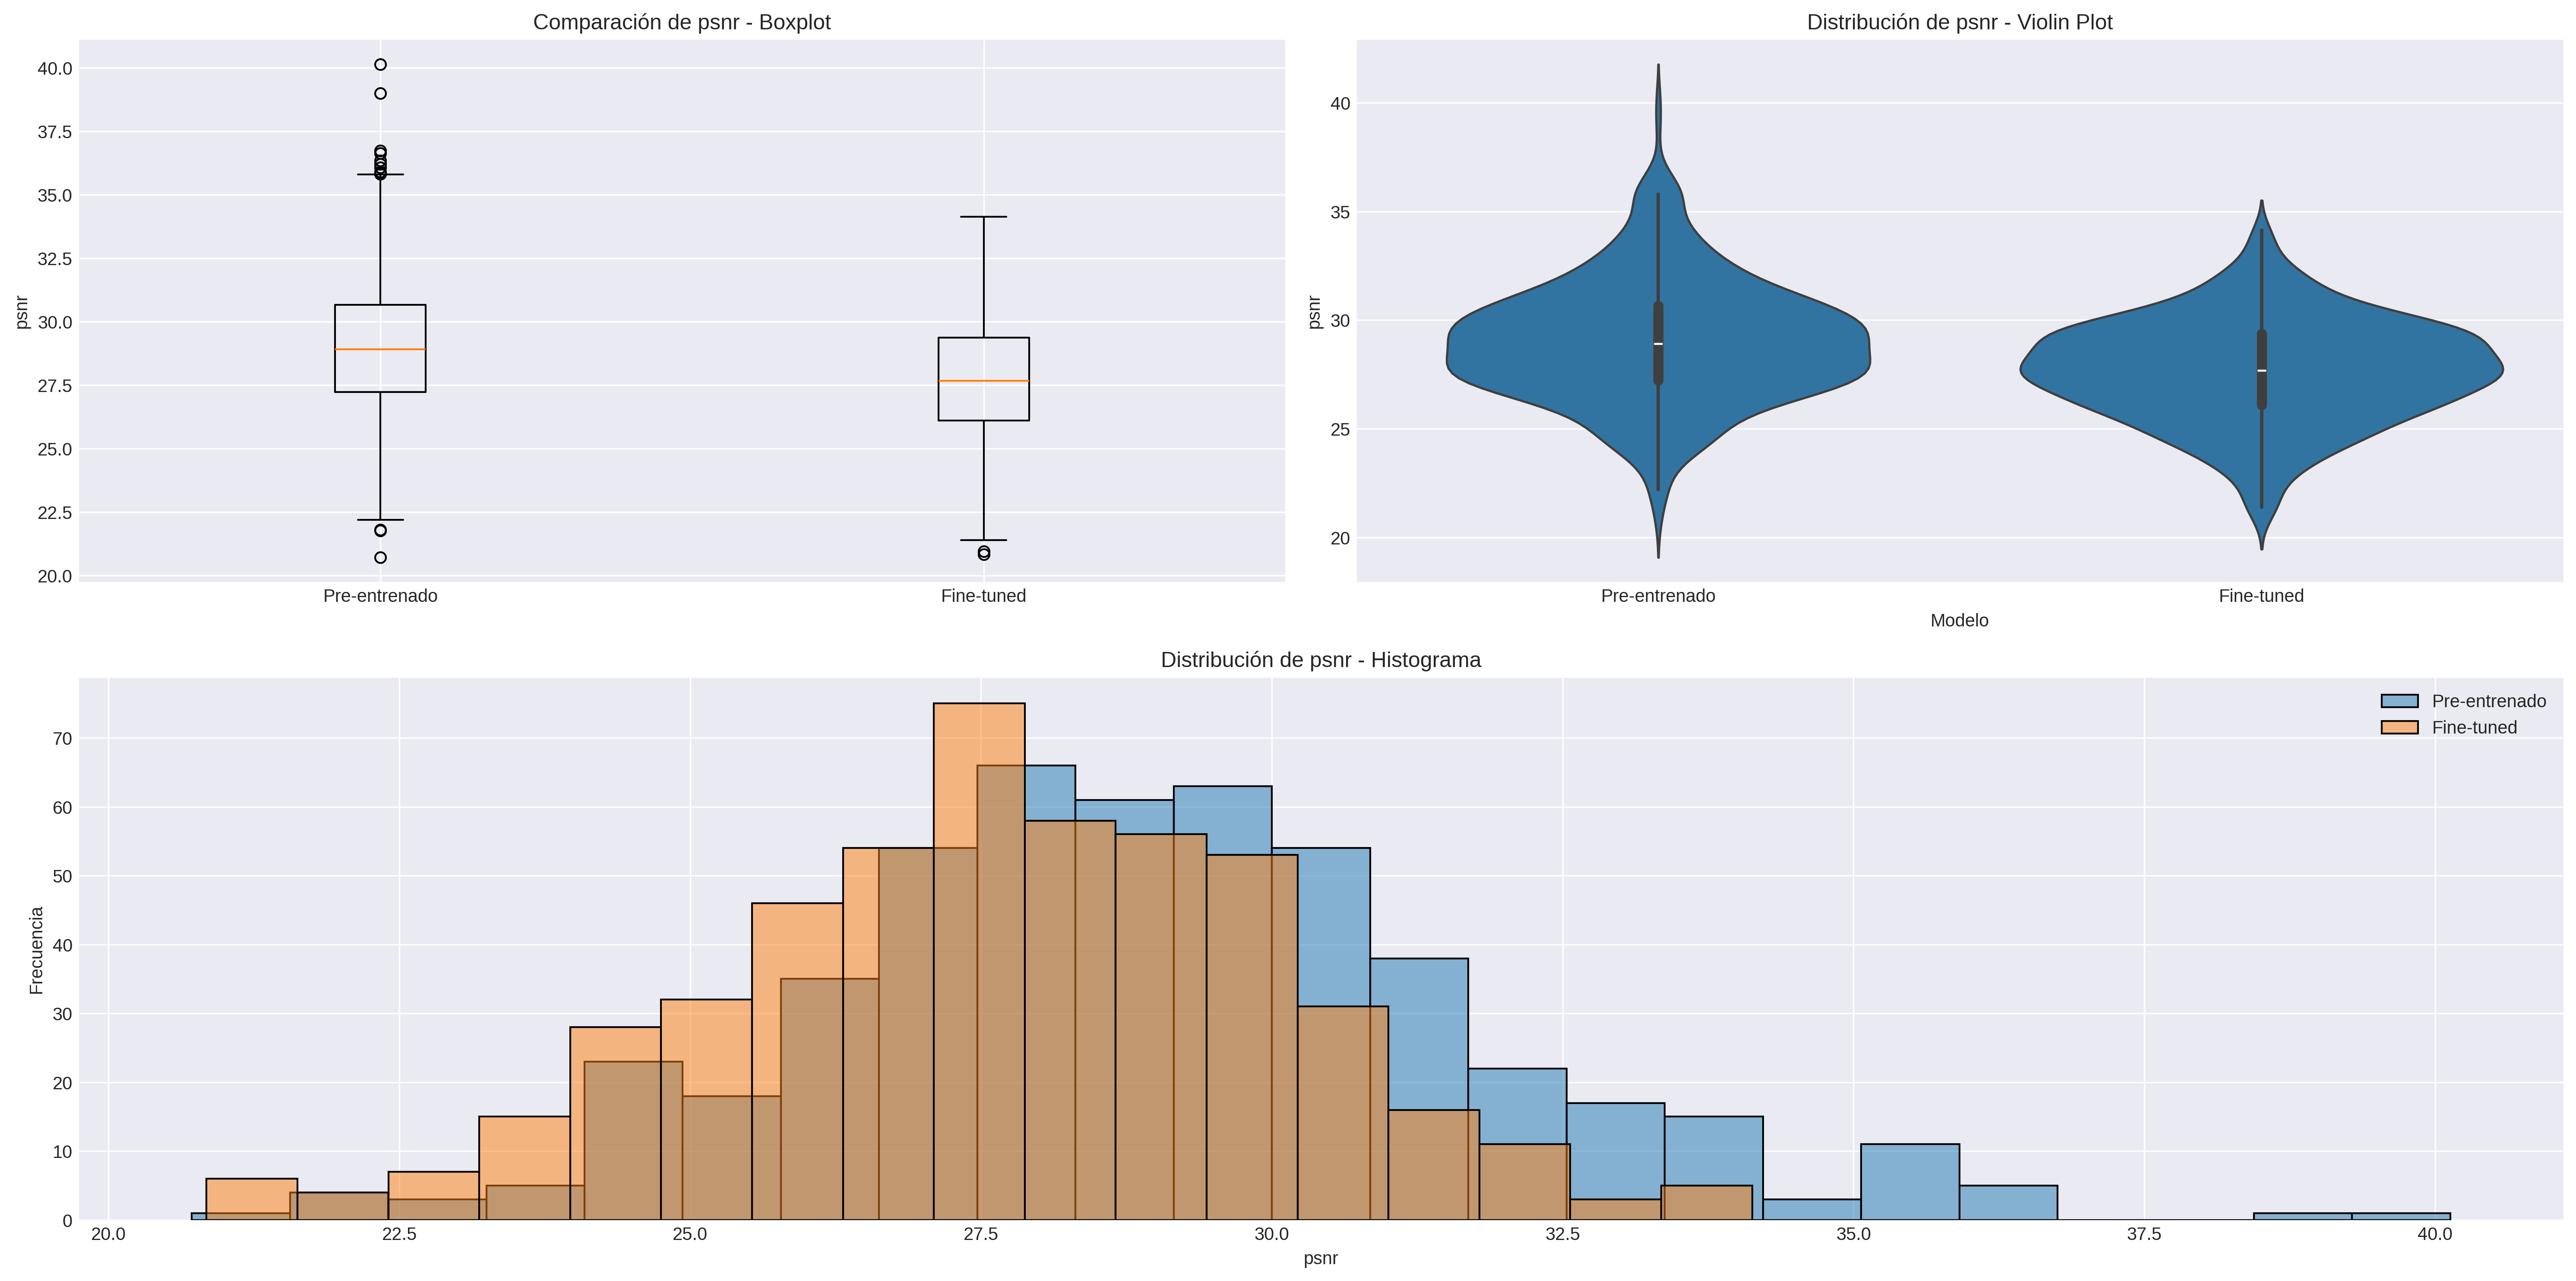
\includegraphics[width=\textwidth]{Images/comparison_plots_psnr_no_struct.png}
        \caption{Comparación entre fine-tuning sin componente estructural y modelo pre-entrenado}
        \label{fig:psnr_violin}
    \end{subfigure}
    
    \vspace{0.5cm}
    
    \begin{subfigure}[b]{0.7\textwidth}
        \centering
        % FT vs Baseline
        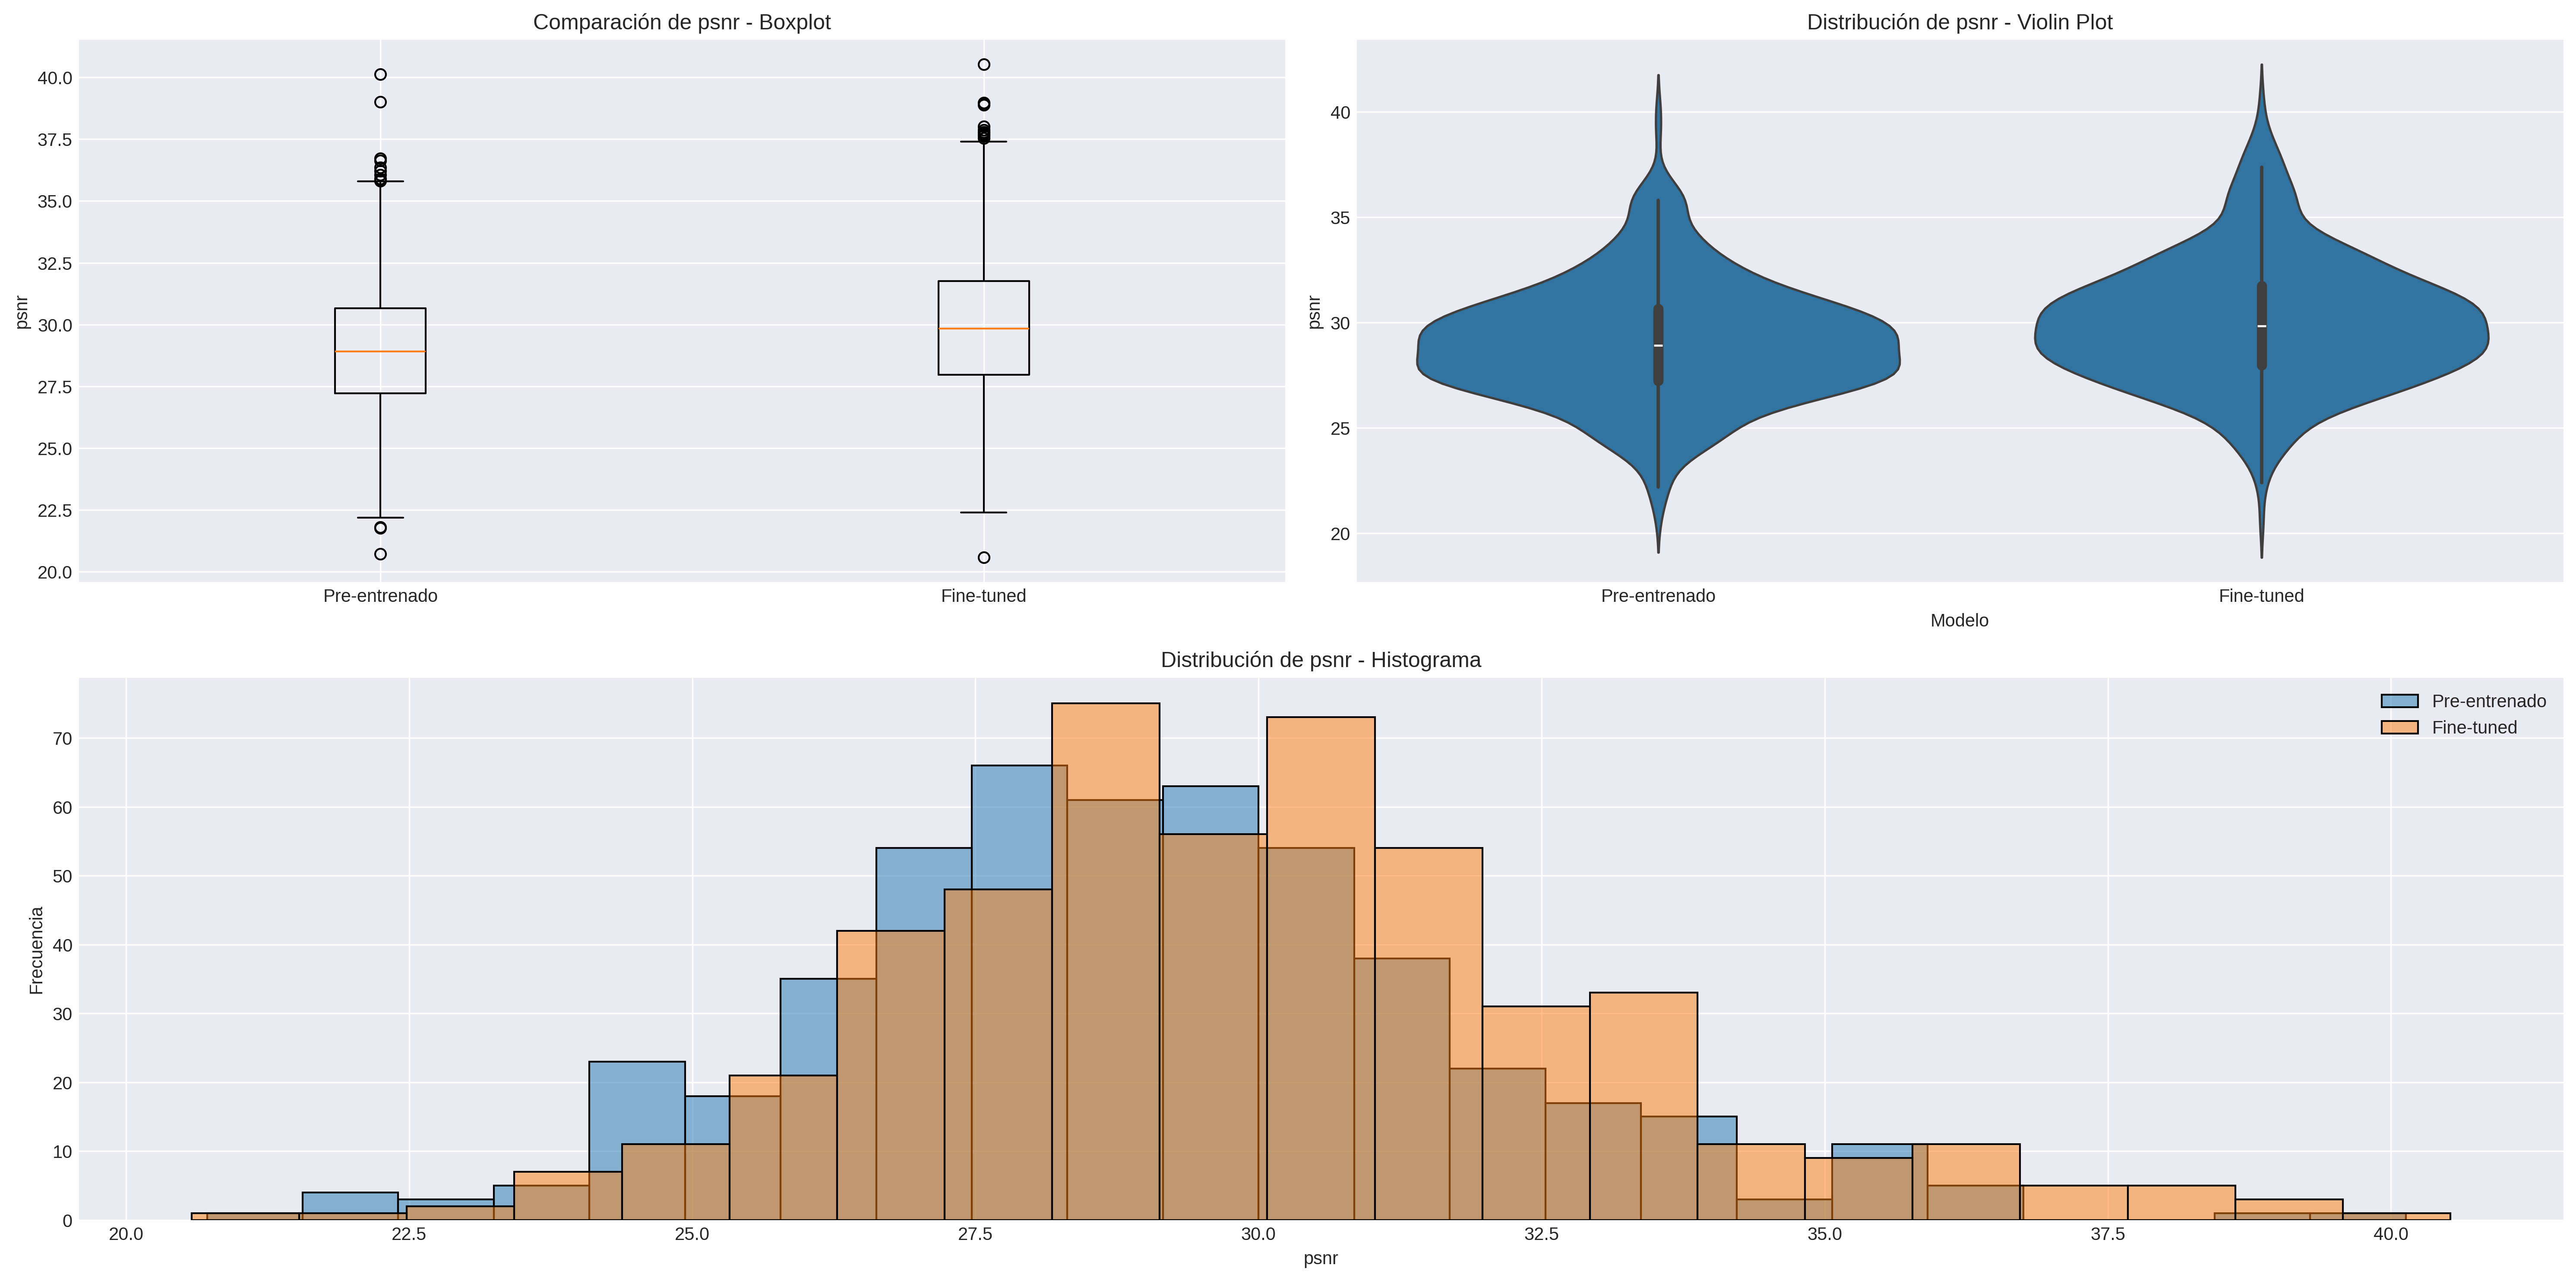
\includegraphics[width=\textwidth]{Images/comparison_plots_psnr_sup.png}
        \caption{Comparación entre fine-tuning (FT) completo y modelo pre-entrenado}
        \label{fig:psnr_box}
    \end{subfigure}
    
    \caption{Análisis comparativo del Peak Signal-to-Noise Ratio (PSNR) entre el modelo pre-entrenado y las variantes de fine-tuning implementadas. a) Comparación entre fine-tuning sin componente física y modelo pre-entrenado. b) Comparación entre fine-tuning sin componente estructural y modelo pre-entrenado. c) Comparación entre fine-tuning completo y modelo pre-entrenado.}
    \label{fig:psnr_analysis}
\end{figure}


\paragraph{Fine-tuning Completo (FT)}
El modelo con fine-tuning completo logra una mejora sustancial en la calidad de reconstrucción según el PSNR. El valor medio aumentó de 29.03 dB en el modelo pre-entrenado a 30.01 dB en el modelo fine-tuned, representando un incremento de aproximadamente 1 dB. Este aumento es significativo en el contexto del PSNR, donde incluso pequeñas mejoras en decibelios pueden representar diferencias notables en la calidad visual de la reconstrucción.

La distribución de los valores de PSNR muestra características interesantes:

\begin{itemize}
    \item Se observa un aumento en el rango dinámico, con el valor máximo mejorando de 40.13 dB a 40.52 dB
    \item La mediana aumentó de 28.92 dB a 29.84 dB, indicando una mejora consistente en la tendencia central
    \item La desviación estándar se incrementó ligeramente de 2.82 dB a 3.01 dB, sugiriendo una mayor variabilidad en la capacidad del modelo para manejar casos difíciles
\end{itemize}

El análisis estadístico confirma la significancia de estas mejoras:

\begin{itemize}
    \item La prueba $t$ pareada ($t = -13.0039$, $p < 0.001$) y la prueba de Wilcoxon ($W = 24581.0000$, $p < 0.001$) demuestran que el incremento en PSNR es estadísticamente significativo
    \item El tamaño del efecto ($d$ de $Cohen = -0.3375$) indica una mejora de magnitud media
    \item Las pruebas de Shapiro-Wilk sugieren ligeras desviaciones de la normalidad en ambas distribuciones
\end{itemize}

\paragraph{Fine-tuning sin Componente Física (FT No-Physical)}
La eliminación de la componente física resulta en una degradación notable de la calidad de reconstrucción. El PSNR medio disminuyó a 28.41 dB, representando una pérdida de aproximadamente 0.62 dB respecto al modelo pre-entrenado. Esta reducción es particularmente relevante porque indica un aumento en el ruido de reconstrucción cuando se omite la información física del proceso de entrenamiento.

Los cambios en la distribución del PSNR son reveladores:

\begin{itemize}
    \item El valor máximo se redujo significativamente a 37.81 dB
    \item La mediana descendió a 28.39 dB
    \item La desviación estándar se mantuvo similar (2.74 dB), sugiriendo que la degradación es consistente a través de diferentes casos
\end{itemize}

Las pruebas estadísticas confirman que este deterioro es significativo ($t = 11.8015$, $p < 0.001$; $W = 25972.0000$, $p < 0.001$), con un tamaño del efecto ($d$ de $Cohen = 0.2237$) que indica un impacto negativo moderado.

\paragraph{Fine-tuning sin Componente Estructural (FT No-Structural)}
La ausencia de la componente estructural produce el deterioro más severo en términos de PSNR. El valor medio cayó a 27.67 dB, representando una pérdida de aproximadamente 1.36 dB respecto al modelo pre-entrenado. Esta disminución sustancial en el PSNR indica un aumento significativo en el ruido de reconstrucción y una pérdida notable de calidad en las imágenes reconstruidas.

El impacto negativo se manifiesta en varios aspectos:

\begin{itemize}
    \item Una reducción dramática en el valor máximo alcanzable (34.13 dB)
    \item Una disminución en la mediana a 27.68 dB
    \item Una reducción en la variabilidad (desviación estándar de 2.38 dB), sugiriendo que el modelo consistentemente produce reconstrucciones de menor calidad
\end{itemize}

El análisis estadístico revela la magnitud del deterioro:

\begin{itemize}
    \item La prueba t pareada muestra un efecto fuerte ($t = 21.0604$, $p < 0.001$)
    \item La prueba de Wilcoxon corrobora estos resultados ($W = 8795.0000$, $p < 0.001$)
    \item El tamaño del efecto ($d$ de $Cohen = 0.5200$) indica un impacto negativo grande
\end{itemize}

Este análisis del PSNR complementa y refuerza las conclusiones obtenidas de las métricas anteriores, proporcionando una perspectiva adicional basada en la relación señal-ruido. Los resultados confirman que tanto la componente física como la estructural son cruciales para mantener una alta calidad de reconstrucción, siendo la componente estructural particularmente crítica para preservar la fidelidad de la señal reconstruida.


\subsubsection{Índice de Similitud Estructural (SSIM)}

El Structural Similarity Index (SSIM) es una métrica que evalúa la calidad de imagen basándose en la percepción humana, considerando la similitud estructural, de luminancia y de contraste entre las imágenes originales y reconstruidas. A diferencia de métricas basadas puramente en error como MSE o MAE, el SSIM está diseñado para alinearse mejor con la percepción visual humana. Los valores de SSIM varían entre 0 y 1, donde 1 representa una coincidencia perfecta entre las imágenes.


\begin{figure}[H]
    \centering
    \begin{subfigure}[b]{0.48\textwidth}
        \centering
        % FT No-Physical vs Baseline
        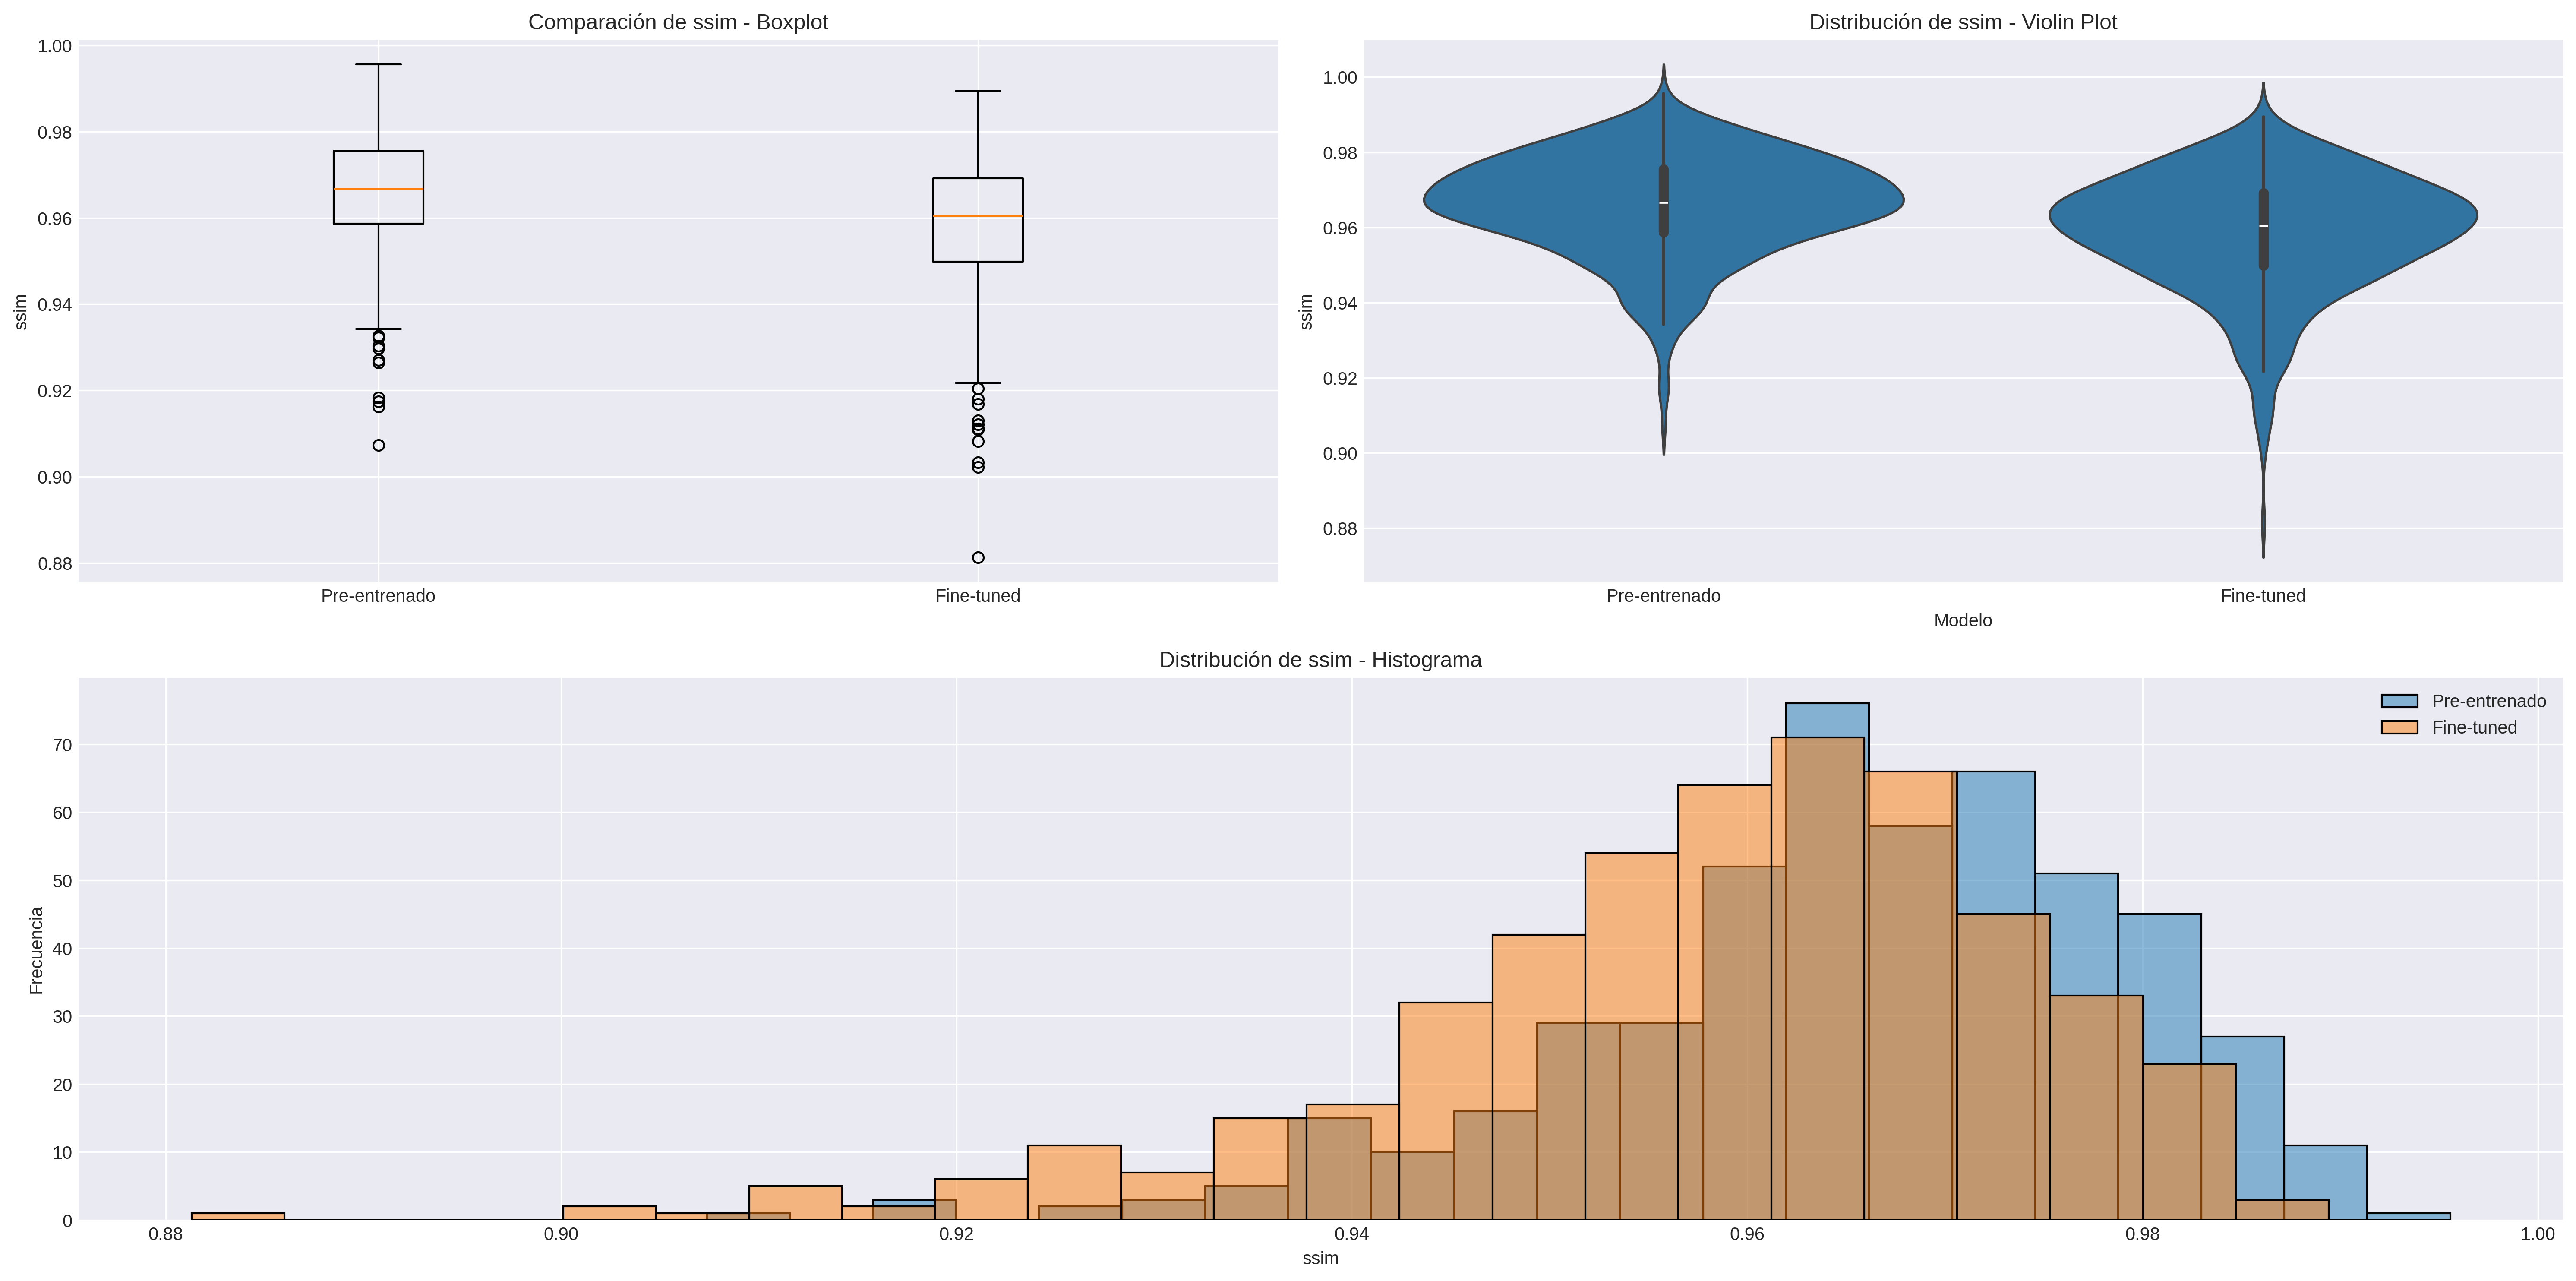
\includegraphics[width=\textwidth]{Images/comparison_plots_ssim_no_phy.png}
        \caption{Comparación entre fine-tuning sin componente física y modelo pre-entrenado}
        \label{fig:ssim_hist}
    \end{subfigure}
    \hfill
    \begin{subfigure}[b]{0.48\textwidth}
        \centering
        % FT No-Structural vs Baseline
        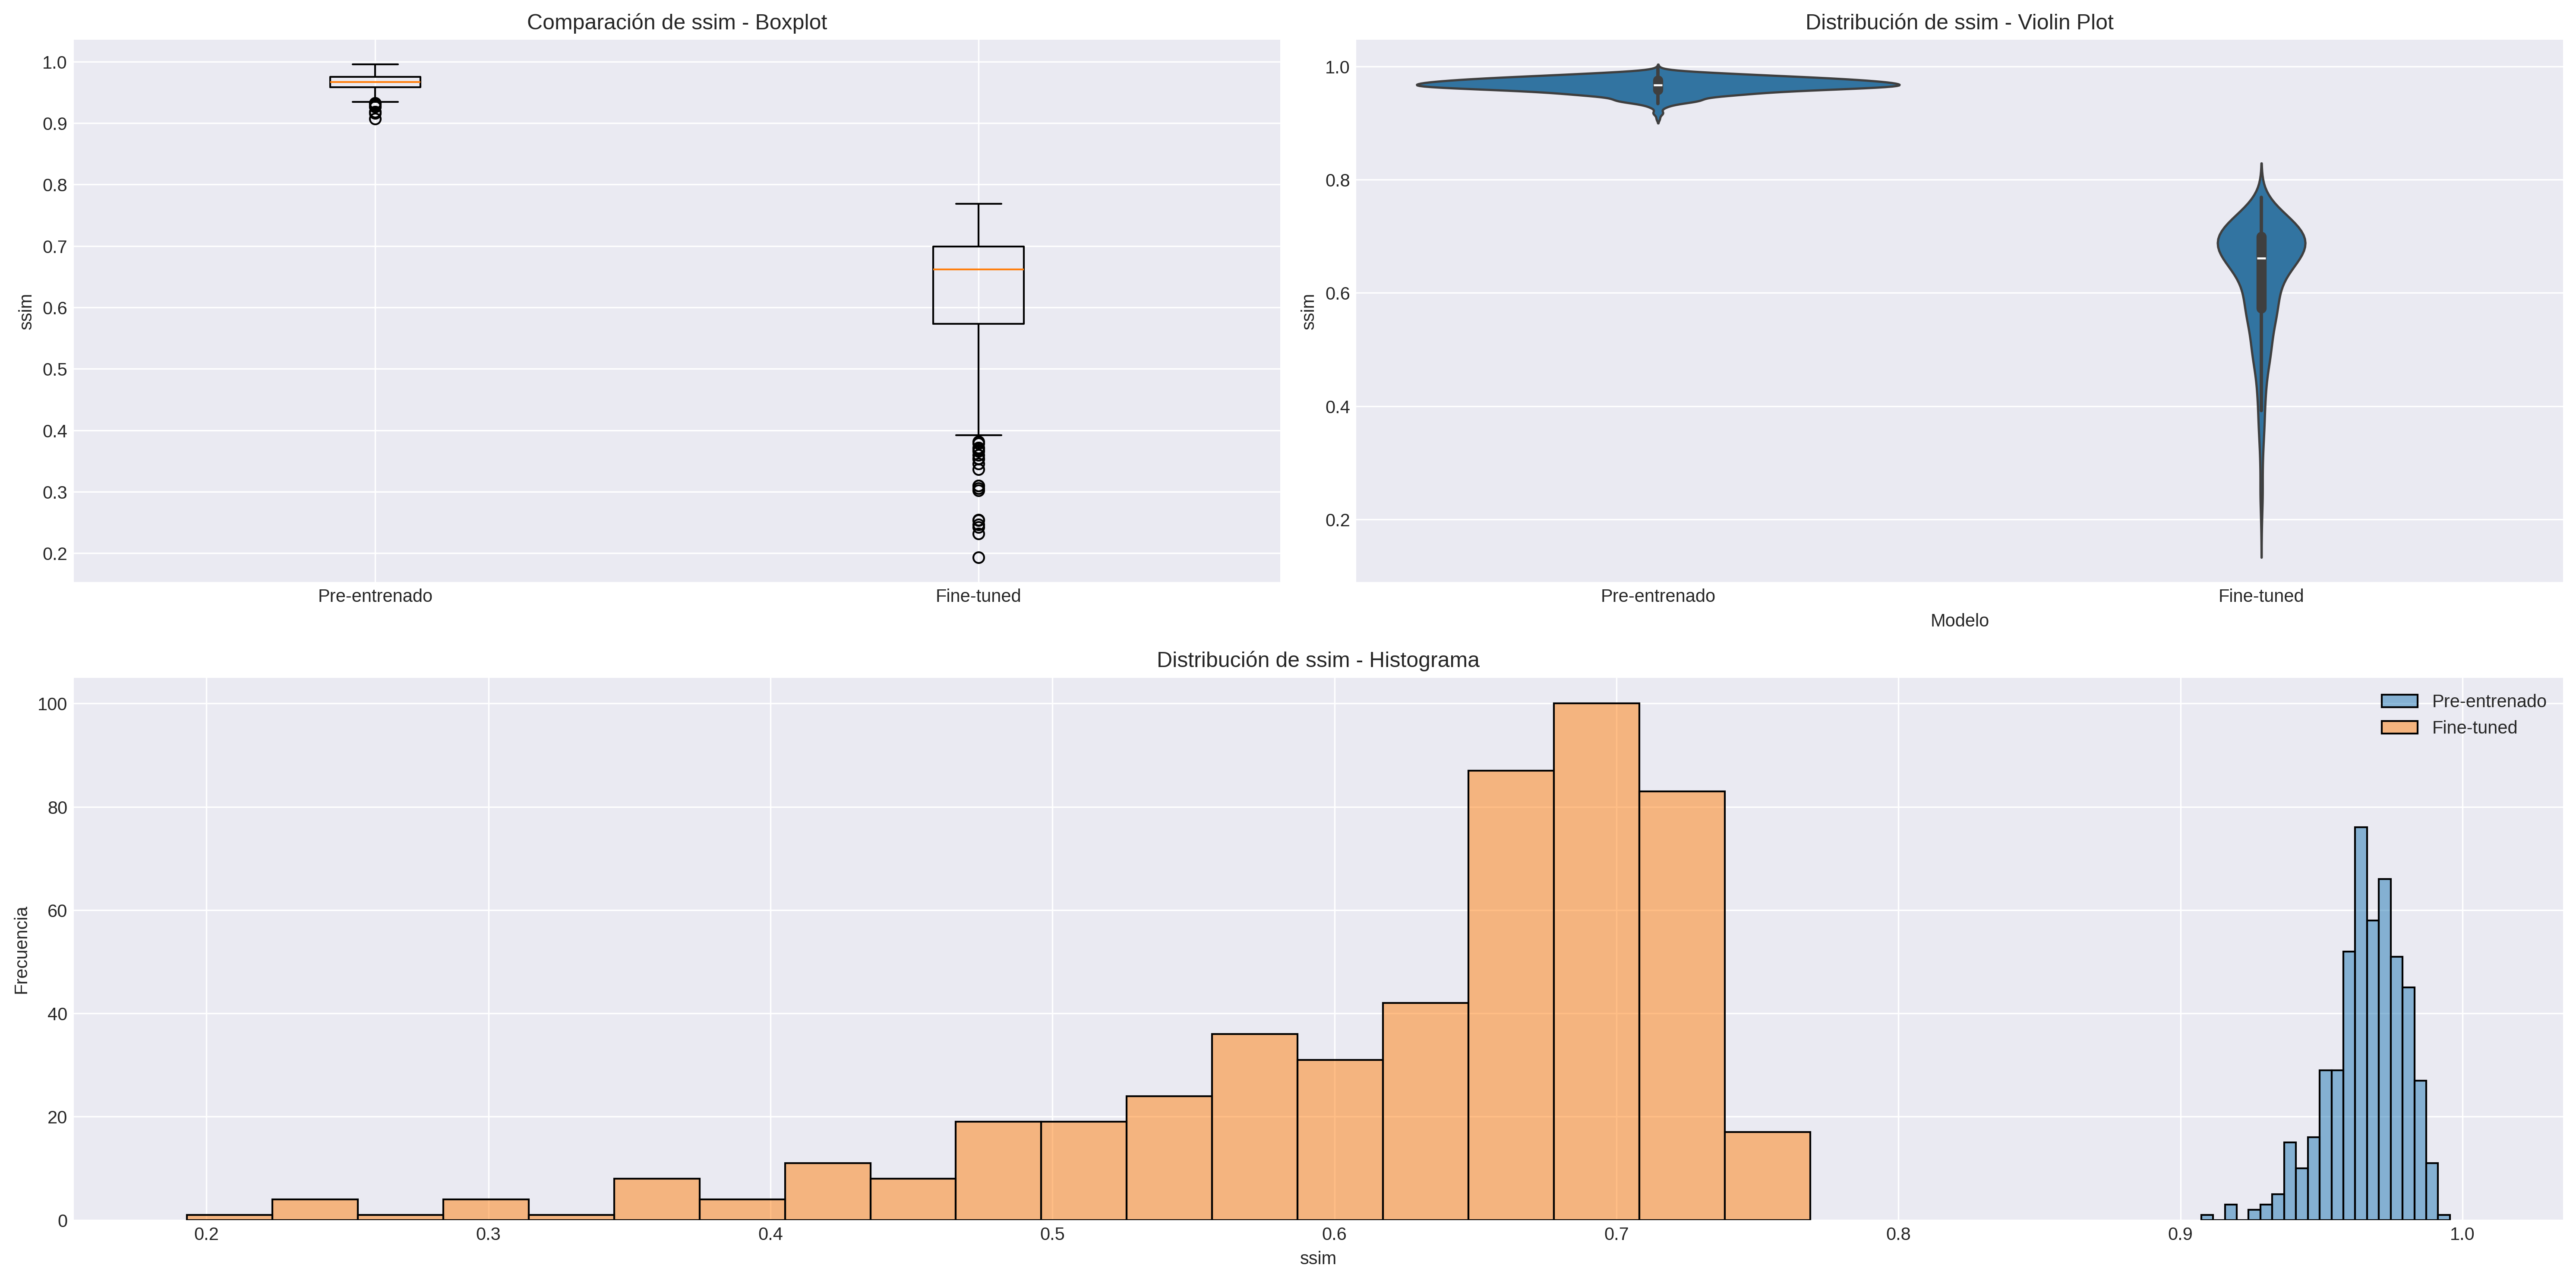
\includegraphics[width=\textwidth]{Images/comparison_plots_ssim_no_struct.png}
        \caption{Comparación entre fine-tuning sin componente estructural y modelo pre-entrenado}
        \label{fig:ssim_violin}
    \end{subfigure}
    
    \vspace{0.5cm}
    
    \begin{subfigure}[b]{0.7\textwidth}
        \centering
        % FT vs Baseline
        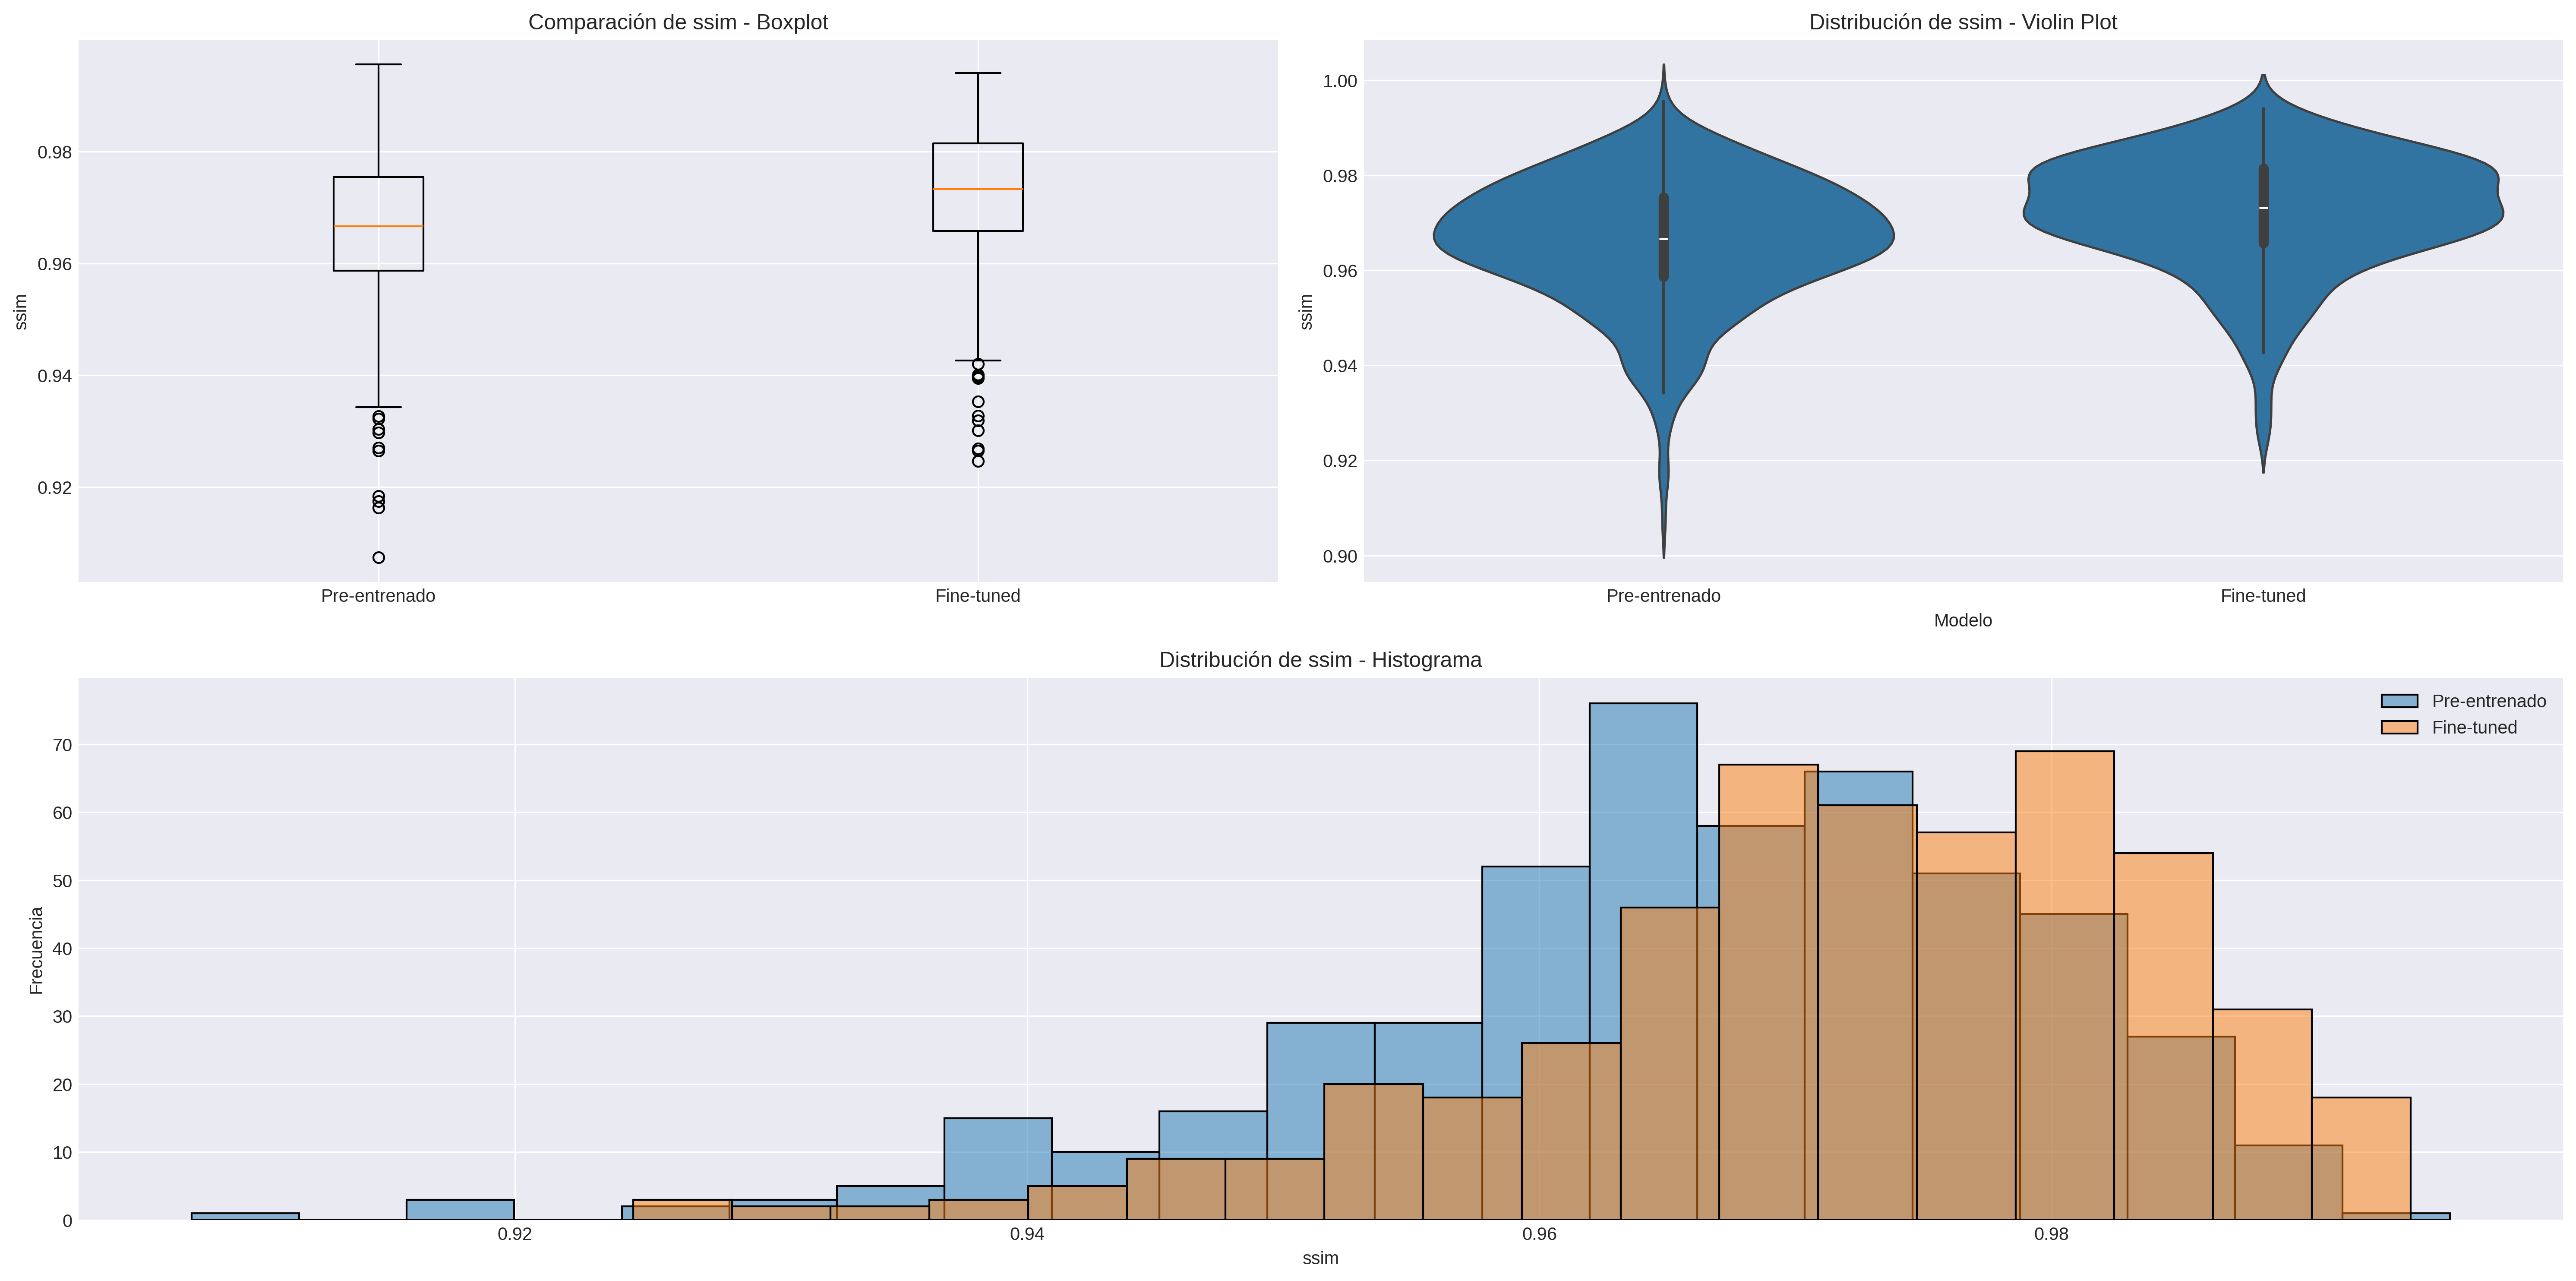
\includegraphics[width=\textwidth]{Images/comparison_plots_ssim_sup.png}
        \caption{Comparación entre fine-tuning (FT) completo y modelo pre-entrenado}
        \label{fig:ssim_box}
    \end{subfigure}
    
    \caption{Análisis comparativo del Índice de Similitud Estructural (SSIM) entre el modelo pre-entrenado y las variantes de fine-tuning implementadas. a) Comparación entre fine-tuning sin componente física y modelo pre-entrenado. b) Comparación entre fine-tuning sin componente estructural y modelo pre-entrenado. c) Comparación entre fine-tuning completo y modelo pre-entrenado.}
    \label{fig:ssim_analysis}
\end{figure}


\paragraph{Fine-tuning Completo (FT)}
El modelo con fine-tuning completo logra una mejora significativa en la calidad perceptual de las reconstrucciones. El SSIM medio aumentó de 0.9658 en el modelo pre-entrenado a 0.9721 en el modelo fine-tuned, lo que representa una mejora en la similitud estructural. Aunque este incremento pueda parecer modesto en términos absolutos, es importante contextualizar que estos valores ya están muy cerca del máximo teórico de 1.0, lo que hace que cualquier mejora en este rango sea particularmente significativa.

La calidad y consistencia de las reconstrucciones se refleja en varios aspectos:

\begin{itemize}
    \item La mediana mejoró de 0.9666 a 0.9732, indicando una mejora sistemática en la tendencia central
    \item La variabilidad se redujo, con una disminución en la desviación estándar de 0.0135 a 0.0123
    \item El valor mínimo aumentó de 0.9074 a 0.9246, sugiriendo una mejor capacidad para manejar casos difíciles
    \item El valor máximo se mantuvo muy alto, cercano a 0.99 en ambos casos
\end{itemize}

El análisis estadístico confirma la significancia de estas mejoras:

\begin{itemize}
    \item La prueba t pareada $(t = -18.8183, p < 0.001)$ y la prueba de Wilcoxon $(W = 14074.0000, p < 0.001)$ demuestran que la mejora es estadísticamente significativa
    \item El tamaño del efecto $(d$ de $Cohen = -0.4819)$ indica un impacto positivo de magnitud media a grande
    \item Las pruebas de Shapiro-Wilk revelan desviaciones de la normalidad en ambas distribuciones, subrayando la importancia de las pruebas no paramétricas
\end{itemize}

\paragraph{Fine-tuning sin Componente Física (FT No-Physical)}
La eliminación de la componente física resulta en una degradación leve pero significativa de la calidad estructural. El SSIM medio disminuyó a 0.9583, representando una pérdida relativamente pequeña pero estadísticamente significativa. Este resultado sugiere que la componente física, aunque importante, no es crítica para mantener la similitud estructural básica entre las imágenes originales y reconstruidas.

Los cambios en la distribución del SSIM son sutiles pero notables:

\begin{itemize}
    \item La mediana descendió levemente a 0.9605
    \item Se observó un ligero aumento en la variabilidad (desviación estándar de 0.0157)
    \item El valor mínimo disminuyó a 0.8813, indicando una mayor dificultad con casos desafiantes
\end{itemize}

Las pruebas estadísticas confirman la significancia de estos cambios:

\begin{itemize}
    \item El estadístico $t$ de $25.0947$ ($p < 0.001$) y el estadístico de Wilcoxon $W = 3218.0000$ ($p < 0.001$) indican diferencias significativas
    \item El tamaño del efecto ($d$ de $Cohen = 0.5123$) sugiere un impacto negativo substancial
\end{itemize}

\paragraph{Fine-tuning sin Componente Estructural (FT No-Structural)}
La ausencia de la componente estructural produce un deterioro dramático en la calidad perceptual de las reconstrucciones. El SSIM medio cayó significativamente a 0.6257, representando una degradación masiva en la similitud estructural. Esta caída de más de 0.34 puntos es particularmente alarmante dado que el SSIM es una métrica que típicamente muestra cambios más sutiles.

El impacto devastador se manifiesta en múltiples aspectos:

\begin{itemize}
    \item Una caída dramática en el valor máximo a 0.7688, muy por debajo del rango típico de calidad aceptable
    \item Un valor mínimo extremadamente bajo de 0.1930, indicando casos de reconstrucción muy deficiente
    \item Un aumento masivo en la variabilidad (desviación estándar de 0.1041), sugiriendo una pérdida de consistencia en la calidad de reconstrucción
\end{itemize}

El análisis estadístico revela la magnitud sin precedentes de este deterioro:

\begin{itemize}
    \item La prueba t pareada muestra un efecto extremadamente fuerte ($t = 76.6244$, $p < 0.001$)
    \item La prueba de Wilcoxon ($W = 0.0000$, $p < 0.001$) confirma la uniformidad del deterioro
    \item El tamaño del efecto ($d$ de $Cohen = 4.5827$) indica un impacto negativo excepcionalmente grande
\end{itemize}

Este análisis del SSIM proporciona una perspectiva crucial centrada en la calidad perceptual de las reconstrucciones. Los resultados demuestran de manera contundente que la componente estructural es absolutamente esencial para mantener la fidelidad visual de las reconstrucciones, mientras que la componente física juega un papel más sutil pero significativo. La caída dramática en el SSIM al eliminar la componente estructural sugiere que esta pérdida no solo afecta métricas numéricas sino que también tiene un impacto sustancial en la calidad visual percibida de las reconstrucciones.

\subsection{Predicciones}

En esta sección, se presentan los resultados de las predicciones realizadas por el modelo pre-entrenado y los modelos fine-tuned en el conjunto de datos de validación. Las predicciones se comparan con los valores reales para evaluar la capacidad de los modelos para generalizar a datos no vistos. Se analizan las distribuciones de los errores de predicción y se realizan pruebas estadísticas para evaluar la significancia de las diferencias entre los modelos.


\begin{figure}[H]
    \centering
    \begin{subfigure}[b]{0.8\textwidth}
        \centering
        % Baseline 
        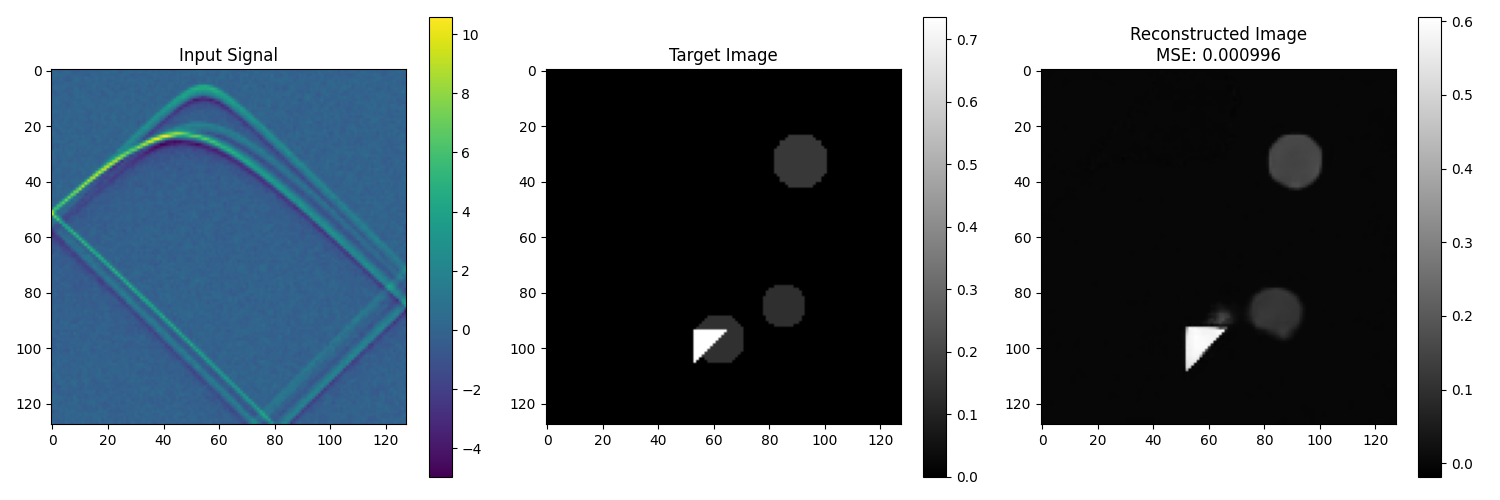
\includegraphics[width=\textwidth]{Images/sample_solo.png}
        \caption{Ejemplo de predicciones realizadas por el modelo pre-entrenado.}
        \label{fig:sample_solo}
    \end{subfigure}

    \vspace{0.5cm}
    
    \begin{subfigure}[b]{0.8\textwidth}
        \centering
        % FT (Full)
        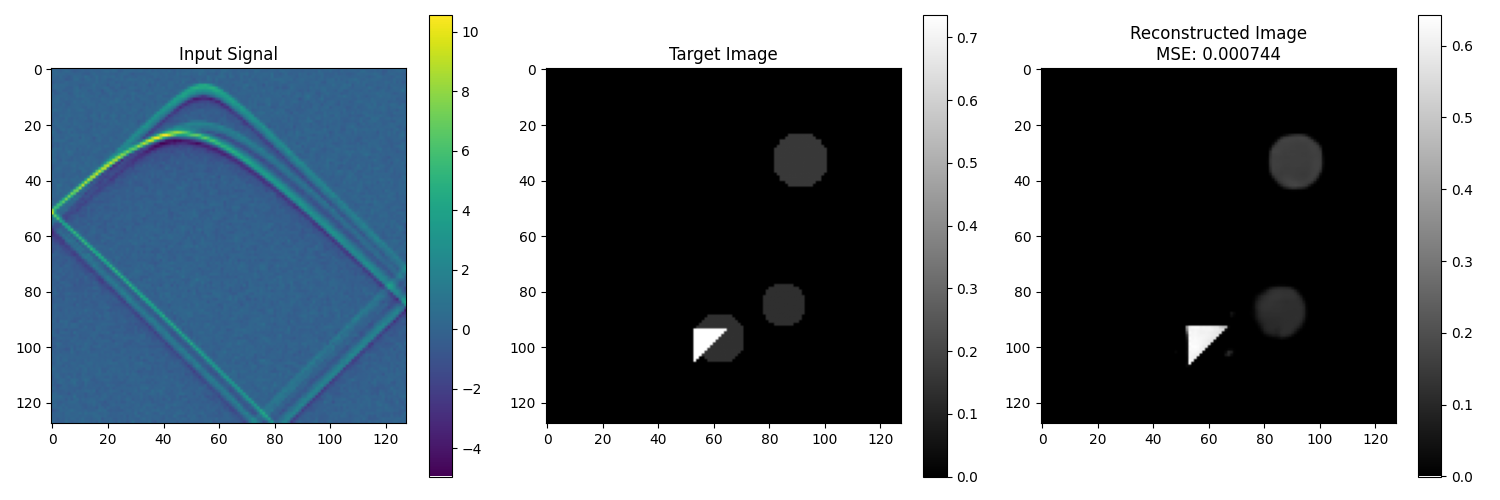
\includegraphics[width=\textwidth]{Images/sample_sup.png}
        \caption{Ejemplo de predicciones realizadas por el modelo fine-tuned completo.}
        \label{fig:sample_sup}
    \end{subfigure}
    
    \vspace{0.5cm}
    
    \begin{subfigure}[b]{0.8\textwidth}
        \centering
        % FT (No-Structural)
        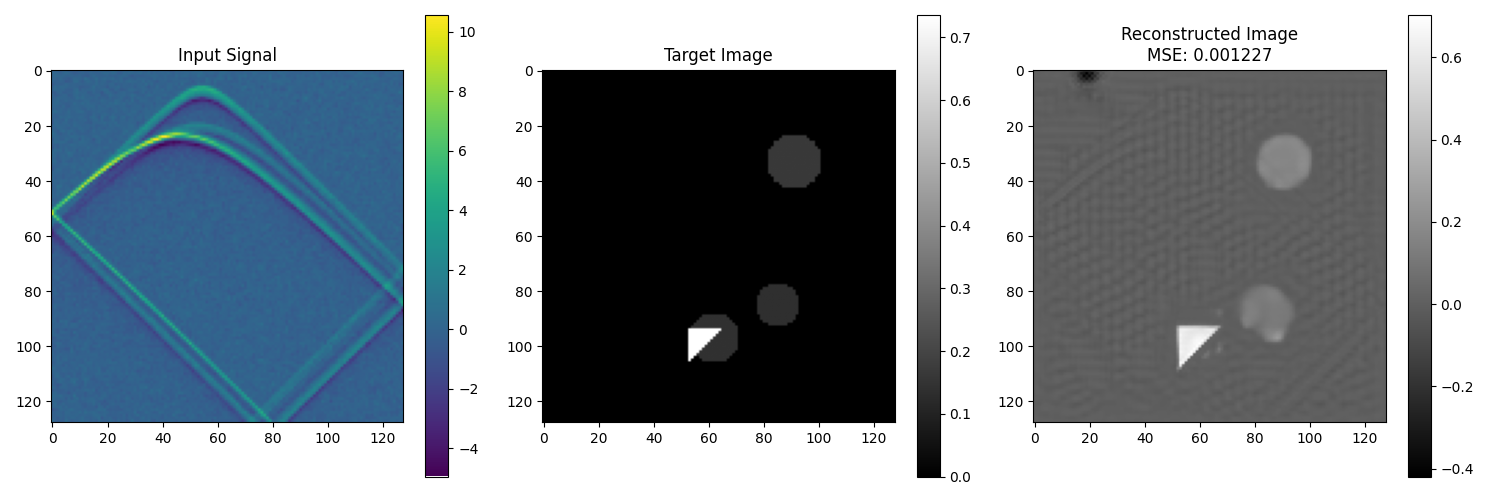
\includegraphics[width=\textwidth]{Images/sample_no_struct.png}
        \caption{Ejemplo de predicciones realizadas por el modelo fine-tuned sin componente estructural.}
        \label{fig:sample_no_struct}
    \end{subfigure}
    
    \begin{subfigure}[b]{0.8\textwidth}
        \centering
        % FT (No-Physical)
        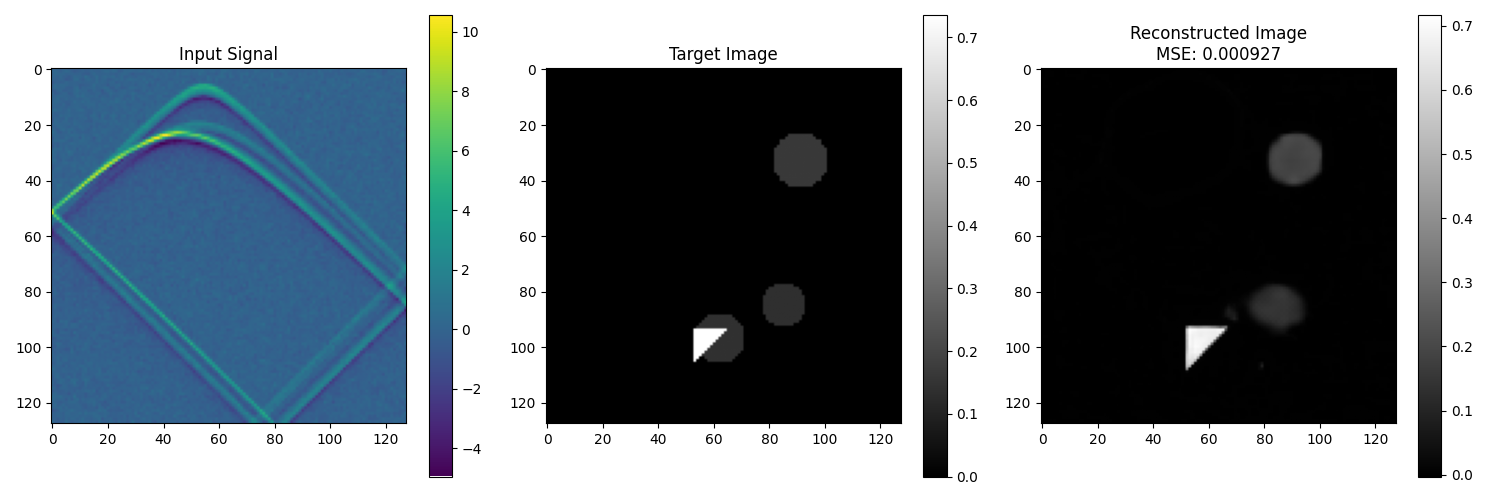
\includegraphics[width=\textwidth]{Images/sample_no_phy.png}
        \caption{Ejemplo de predicciones realizadas por el modelo fine-tuned sin componente física.}
        \label{fig:sample_no_phy}
    \end{subfigure}

    \caption{Ejemplos de predicciones realizadas por el modelo pre-entrenado y los modelos fine-tuned en el conjunto de datos de validación.}
    \label{fig:sample_analysis}
\end{figure}



